\documentclass[11pt]{article}

\usepackage[margin=1in]{geometry}
\usepackage[T1]{fontenc}
\usepackage{amsmath}
\usepackage{amssymb}
\usepackage{amsthm}
\usepackage{graphicx}
\usepackage{float}
\usepackage{booktabs}
\usepackage{tabularx}
\usepackage{algorithm}
\usepackage{algpseudocode}
\usepackage{tikz}
\usetikzlibrary{positioning,arrows.meta,shapes,fit,backgrounds}
\usepackage[font={small,sf},labelfont={bf,sf},labelsep=period,margin=8pt]{caption}
\usepackage[hidelinks]{hyperref}
\usepackage{url}
\usepackage{siunitx}
\usepackage{microtype}
\usepackage{rotating}
\usepackage[numbers,sort&compress]{natbib}

\newtheorem{conjecture}{Conjecture}

% Product-name macros. Rendered in small caps so named objects stand out from
% prose, following the convention used in Byrd et al. (ABIDES), Frey et al.
% (JAX-LOB), and similar simulator papers.
\newcommand{\kasparhft}{\textsc{Kaspar-HFT}}
\newcommand{\shadowpov}{\textsc{Shadow-POV}}

\title{Modelling Latency Tails in an Order-Book Simulator Driven by Hawkes-Clustered CME MDP3 Arrivals}
\author{Vincent Mayeski\thanks{M2 Tech (16425640 Canada Inc.), Montreal. \texttt{v@m2te.ch}}}
\date{Draft, September 18, 2026}

\begin{document}

\maketitle

\begin{abstract}
Limit-order-book (LOB) simulators are the default environment in which high-frequency trading algorithms are evaluated, and the reported profit-and-loss of a candidate strategy is only as trustworthy as the simulator's latency model. Published simulators uniformly treat per-message latency as a constant scalar, an i.i.d. draw from a supplied distribution, or the outcome of a real network fabric between simulated agents, decoupled from the order-flow arrival process. On the raw feed of the Chicago Mercantile Exchange's Market Data Platform version 3 (CME MDP3), a public multicast market-data feed carrying tick-by-tick book updates and trades for CME futures contracts, the arrival process is strongly Hawkes-clustered \citep{hawkes1971spectra,bacry2015review}. Under any downstream service queue, Hawkes-clustered arrivals produce heavy-tailed system latency \citep{dawpender2018queues}. A constant-delay simulator cannot reproduce this behaviour and will misprice any strategy whose profit-and-loss is sensitive to burst-conditioned latency.

This paper quantifies the misprice and provides the minimal correction. Three per-window latency tail statistics are measured on approximately 281 sessions of the E-mini NASDAQ-100 (CME symbol NQ) front-month contract covering 2025-01 to 2026-02: matching-engine latency, send-to-handler latency, and the system time of a modelled single-server queue with deterministic service driven by the observed handler-end arrival stream. Exponential Hawkes fits per 30-minute window supply the branching ratio $n$ and the long-run intensity $\bar\lambda$ used to condition the three tails on a $5 \times 5$ equal-quantile grid. The measurement pipeline is then used to upgrade the \kasparhft{} simulator \citep{mayeski_actorhft},\footnote{Companion source repository: \url{https://github.com/m2tech/kaspar-hft} (placeholder --- final URL to be confirmed).} a discrete-event MDP3 replay simulator built on the actor-based execution framework of the same name and maintained at M2 Tech: its constant per-message release rule is replaced on each side by the Lindley recursion of a single-server queue with deterministic service, parametrised by an inbound and an outbound service time. The inbound service time is supplied by the operator from instrumentation of the receive path; the outbound service time is estimated from a low quantile of the public matching-engine-to-gateway latency distribution.

The load-bearing experiment is a pair of parameter sweeps on \shadowpov{} \citep{mayeski2026shadowpov}, a specific percentage-of-volume (POV) execution algorithm \citep{konishimakimoto2001pov} previously deployed and evaluated at M2 Tech on CME futures. Sweep one varies the level of a constant per-message delay across two orders of magnitude in the microsecond band and reports fill rate against that scalar; sweep two varies the system inbound service-time parameter of the two-queue Lindley recursion and reports fill rate against that scalar under the same tape and random seed. The paper's practitioner deliverable is the quantitative measurement of these two sensitivities. For a POV-family algorithm whose decisions run on accumulated volume signals rather than microsecond races, both sensitivities are expected to be small; reporting them precisely places a quantitative bound on how much engineering effort the algorithm can profitably absorb before hitting diminishing returns, and provides a template that race-sensitive algorithms --- market makers with adverse-selection avoidance, latency arbitrage strategies --- can apply on the same simulator to obtain their own, expected-larger, sensitivity numbers. Heavy-tailed return and adverse-selection distributions on the same instrument are established prior art \citep{bacry2015review,hardiman2013,carteajaimungalricci2014} and are not re-measured. Companion code contains the message-tape parser, the per-window panel builder, the calibration script for the exchange service time, and the \kasparhft{} simulator with its two-queue upgrade.
\end{abstract}

\clearpage
\tableofcontents
\clearpage
\listoffigures
\listoftables
\clearpage

\section{Introduction}
\label{sec:intro}

\subsection{Motivation}
\label{sec:motivation}

Limit-order-book simulators are the standard evaluation environment for market-making and execution algorithms in both academic and industrial research, and the reported profit-and-loss of a candidate strategy in such a simulator is only as trustworthy as its latency model. Table~\ref{tab:simulators} lists sixteen simulators with public references and code, together with the latency model each employs. Every entry treats latency as constant, as i.i.d. from a supplied distribution, or as the emergent behaviour of a real network transport layer between simulated agents. In no case is latency modelled as the response of a service queue driven by the order-flow arrival process.

On CME MDP3 order-flow data the arrival process is Hawkes-clustered, with branching ratio close to unity across the trading day. Under any downstream service queue, Hawkes-clustered arrivals produce heavy-tailed system latency \citep{dawpender2018queues}. A simulator that assigns constant latency to individual messages cannot reproduce this behaviour and will underestimate the tail latency experienced by algorithms exposed to bursts. The concrete consequence for the practitioner is direct: strategies whose profit-and-loss depends on how quickly a passive quote can be pulled during a burst, on how deep an aggressive order-of-a-fixed-participation-rate will fill against a suddenly-widening book, or on the shape of adverse-selection markouts on fast passive fills, are mispriced by a constant-delay simulator in a way that a more realistic latency model corrects. This paper measures the realistic latency behaviour and quantifies the mispricing.

\begin{sidewaystable}
\centering
\scriptsize
\caption{LOB simulators with public references and code.}
\label{tab:simulators}
\begin{tabular}{@{}p{1.9cm}p{1.9cm}p{2.2cm}p{1.9cm}p{2.1cm}p{3.1cm}p{3.1cm}p{3.0cm}@{}}
\toprule
Simulator & Reference & Language & Book & Tape replay & Latency model & Market impact & Order-flow source \\
\midrule
ABIDES & \citet{byrd2020abides} & Python & MBP synth & No & Per-pair configurable, ns kernel & Book-walking plus reactive agent population & ZI, MM, HFT archetypes \\
ABIDES-Markets, ABIDES-Gym & \citet{amrouni2021abidesgym} & Python & MBP synth & Optional via world agent & Same as ABIDES & Same, plus CGAN world agent for statistical impact & Additional RL and strategic agents \\
MarketSim, PyMarketSim & \citet{masciolwellman2024pymarketsim} & Python & MBP synth & No & Fixed cross-venue delay & Book-walking plus strategic reactive agents & Strategic MM, arbitrage, ZI, RL \\
MAXE & \citet{belcak2020maxe} & C++ core with Python API & MBP incl. pro-rata & No & Explicit per-agent computation and message delays & Book-walking plus agent reaction & Configurable agent pool \\
BSE & \citet{cliff2018bse} & Python & MBP synth & No & Zero (equidistant agents) & Book-walking plus heterogeneous trader reaction & ZIC, ZIP, GVWY, GDX, AA \\
DBSE & \citet{milescliff2019dbse} & Python with cloud runtime & MBP synth & No & Real WAN latency between cloud regions & Book-walking plus agent reaction & Cloud-distributed clients \\
CoinTossX & \citet{jericevich2022cointossx} & Java core with Julia and Python clients & MBP & Yes & Real network transport (SBE and UDP over Aeron) & Book-walking against external clients & External programmatic clients \\
LOBSTER & \citet{huangpolak2011lobster} & Data with Python and MATLAB helpers & MBO & Playback & Not applicable & None (passive reconstruction) & Historical NASDAQ ITCH \\
JAX-LOB & \citet{frey2023jaxlob} & Python with JAX and GPU & MBP & Yes & None & Book-walking against replayed queue & RL policies pluggable \\
JaxMARL-HFT & \citet{mohl2025jaxmarl} & Python with JAX & MBO & Yes & Fixed order-latency parameter & Book-walking on replay; no counter-reaction & Multi-agent RL (execution and MM) \\
mbt\_gym & \citet{jerome2023mbtgym} & Python (vectorised) & Model-based (Cartea-Jaimungal family) & No & Optional constant delay & Parametric temporary and permanent impact kernels (Almgren-Chriss) & Single RL agent against stochastic flow \\
Queue-Reactive & \citet{noble2026reality} & C++ & MBP (Markov jump) & Databento MBP-10, INTC, VZ, T, PFE & State-conditioned Markov jump; GMM inter-event distribution; race-based fill rule at $\sim 29\,\si{\micro\second}$ mode & Power-law feedback kernel with concave impact and partial reversion & Empirical event-conditional Markov process \\
Hawkes-LOB & \citet{elkarmi2025hawkeslob} & C++ & MBP & Calibrated to Binance BTCUSDT and LOBSTER AAPL & Event timing driven by Hawkes kernel & Endogenous via self-exciting flow & Multivariate marked Hawkes process \\
DeepMarket, TRADES & \citet{berti2025deepmarket} & Python (PyTorch on ABIDES) & MBP synth & Warm-start from real data & Inherits ABIDES latency model & Diffusion world-agent reacts to test orders & Trained diffusion generator with optional ABIDES agents \\
StockSharp & \citet{stocksharp} & C\# and .NET & MBP & Yes (historical, L2 replay) & Broker-emulated order-book queue & Book-walking; no market reaction to test orders & External strategy modules \\
\kasparhft{} (this work) & --- & C++20 & MBP or MBO & Yes (raw MDP3) & Constant baseline, G/D/1 upgrade & None; orders execute against the replayed book without moving it & Percentage-of-volume executor \\
\bottomrule
\end{tabular}
\end{sidewaystable}

\subsection{Contributions}
\label{sec:contributions}

The load-bearing contribution is the strategy-performance comparison of the paper's headline experiment:

\begin{enumerate}
    \item A pair of parameter sweeps on \shadowpov{} \citep{mayeski2026shadowpov} inside the \kasparhft{} simulator, on the same tape and with the same random seed at every sweep point (Section~\ref{sec:experiment}). Sweep one varies a constant per-message delay $\delta$ across two orders of magnitude in the microsecond band; sweep two varies the outbound service-time parameter $s_{\mathrm{out}}$ of the two-queue Lindley recursion. Fill rate against each parameter is reported in aggregate and per grid cell. Separating the two sweeps distinguishes sensitivity to the level of latency from sensitivity to the tail of latency generated by the queue driven by the Hawkes-clustered arrival process. This separation is the practitioner-relevant deliverable and the reason the rest of the machinery exists.
\end{enumerate}

The remaining four contributions supply the pipeline required to make that comparison honest:

\begin{enumerate}\setcounter{enumi}{1}
    \item A per-window measurement panel of three latency tail statistics on approximately 281 sessions (approximately 2\,800 windows) of CME NQ front-month MDP3, together with the Hawkes parameters $(\bar\lambda, n)$ at 30-minute resolution. The three tails are matching-engine latency, send-to-handler latency, and the system time of a modelled single-server deterministic-service queue driven by the observed handler-end arrival stream.
    \item A $5 \times 5$ equal-quantile analysis of the three tails on the $(\bar\lambda, n)$ plane, reporting absolute cell medians and $p_{99}/p_{50}$ shape ratios.
    \item A minimal upgrade to the \kasparhft{} simulator: replacement of the constant per-message release rule with the Lindley recursion of a single-server deterministic-service queue on each side (inbound market data, outbound orders), parametrised by two scalar service times.
    \item A public calibration procedure for the exchange-side service time from public MDP3 archives.
\end{enumerate}

Heavy-tailed distributions of adverse-selection markouts and short-horizon returns on CME futures are established elsewhere and enter this paper only as prior context: adverse-selection tails in \citet{carteajaimungalricci2014} and related market-making literature, and fat-tailed high-frequency returns in \citet{bacry2015review} and \citet{hardiman2013}. This paper does not re-measure them; it focuses on the effect of the latency stack on strategy performance.

\subsection{Positioning}
\label{sec:positioning}

The theoretical machinery relating Hawkes arrivals to heavy-tailed service-queue backlogs is established in \citet{dawpender2018queues} and its state-dependent extensions \citep{gaozhu2024statedep,koopsboxmamandjes2018}. The application of that machinery to per-firm execution latency inside a discrete-event trading simulator, and the resulting correction to constant-delay backtest results, has not previously been reported.

\subsection{Paper organisation}
\label{sec:organisation}

Section~\ref{sec:related} surveys related work. Section~\ref{sec:data} defines the corpus, the per-window panel, and the $5 \times 5$ grid. Section~\ref{sec:queue} states the queue-latency model and derives its heavy-tailed behaviour from the Hawkes arrival stream. Section~\ref{sec:upgrade} describes the \kasparhft{} simulator upgrade. Section~\ref{sec:experiment} defines the controlled-experiment protocol and reports the resulting deltas. Section~\ref{sec:calibration} gives the practitioner calibration procedure. Section~\ref{sec:discussion} discusses limitations. Section~\ref{sec:future} outlines follow-on work.

\section{Related work}
\label{sec:related}

The paper draws on four bodies of prior work. The first is the design of limit-order-book simulators for evaluation of high-frequency trading algorithms, whose common feature is a decoupled treatment of latency. The second is the empirical measurement of exchange round-trip latency from publicly available order-log data. The third is the queueing-theoretic analysis of single-server queues fed by Hawkes-clustered arrivals, which supplies the theoretical basis for the measurement pipeline and for the \kasparhft{} simulator upgrade proposed here. The fourth is the analytical and empirical evaluation of market-making and execution algorithms under latency assumptions, which supplies the point of comparison for the controlled experiment of Section~\ref{sec:experiment}.

\subsection{Simulator design and its treatment of latency}
\label{sec:related-sim}

The dominant open architecture for LOB simulation in HFT research is ABIDES \citep{byrd2020abides}, a discrete-event simulator with nanosecond kernel resolution and a pluggable population of trading agents. Latency in ABIDES is specified per agent-exchange link as a scalar, optionally drawn once from a supplied distribution, and does not depend on the state of the arrival process. \citet{amrouni2021abidesgym} extend the framework to reinforcement-learning agents, and \citet{coletta2022cgan} subsequently attach a conditional generative adversarial world agent that produces synthetic counter-flow in response to the test agent's actions. \citet{vyetrenko2020getreal} propose stylised-fact realism metrics that ABIDES-class simulators are expected to reproduce; those metrics constrain the marginal distributions of order flow, but not the coupling between arrival intensity and per-message latency, and the ABIDES latency treatment has consequently remained unchanged in the extensions cited.

The strategic agent-based simulators developed by the Wellman group \citep{wahwellman2016,masciolwellman2024pymarketsim} treat latency as a fixed cross-venue delay whose role is to define latency-arbitrage windows and to admit strategic-equilibrium analysis. \citet{belcak2020maxe} introduce MAXE with per-agent computation delays and per-message transport delays; these are configured as scalars specific to each agent and again do not respond to the arrival stream. \citet{cliff2018bse} publishes the Bristol Stock Exchange (BSE) with zero latency between equidistant agents; the cloud-native distributed variant by \citet{milescliff2019dbse} inherits the real WAN delay of the underlying deployment. \citet{jericevich2022cointossx} provide CoinTossX, an open matching engine whose latency is that of the actual network fabric between external programmatic clients; the modelling of latency is therefore delegated to the deployment rather than to the simulator itself.

Two families of simulator built on real order-book data play a special role. LOBSTER \citep{huangpolak2011lobster} is a reconstruction system for NASDAQ ITCH data and contains no trading interface; latency is not applicable. JAX-LOB \citep{frey2023jaxlob} and its multi-agent-RL extension JaxMARL-HFT \citep{mohl2025jaxmarl} apply the replayed order flow to a GPU-parallel book but assign either no latency (JAX-LOB) or a fixed scalar latency (JaxMARL-HFT) to test-agent messages. mbt\_gym \citep{jerome2023mbtgym} is a model-based simulator whose order flow is stochastic rather than replayed, and whose impact model follows the Cartea-Jaimungal family; its latency treatment is again an optional constant. StockSharp \citep{stocksharp} is a broker-emulator style back-tester with a book-queue and no explicit latency model.

Three recent contributions align most closely with the theoretical premise of this paper. The most directly comparable is \citet{noble2026reality}, an extended queue-reactive C++ simulator calibrated on Databento MBP-10 order-flow data for four large-tick U.S. equities. Their construction is a state-conditioned Markov jump process rather than a Hawkes process, but the paper is notable here because it is the first published simulator to explicitly model latency as a first-class object: they identify a mode in the log inter-event-time distribution at approximately 29\,\si{\micro\second}, interpret it as the effective exchange round-trip, and turn it into a race-based fill rule that arbitrates whether the user order fills against the next arrival. Our work differs in that the arrival stream is not synthesised at all: we replay the raw MDP3 tape and place a persistent service-queue backlog on top, so latency is an \emph{ongoing} state driven by the observed arrival stream rather than a one-shot race outcome at fill time. \citet{elkarmi2025hawkeslob} drives event timing directly from a multivariate marked Hawkes process fitted to Binance BTCUSDT trades and LOBSTER AAPL messages; the paper explicitly disclaims latency modelling and its Hawkes intensity is decoupled from queue state. \citet{berti2025deepmarket} train a diffusion world-agent on top of ABIDES that reacts to test orders as a statistical counter-flow; the underlying ABIDES latency model is inherited unchanged.

Across the sixteen simulators of Table~\ref{tab:simulators}, no published architecture treats per-message latency as the response of a service queue whose input is the arrival stream. The contribution of Section~\ref{sec:upgrade} is to close this gap with a minimal recursion applied to the two release queues already present in a conventional discrete-event replay simulator.

\subsection{Empirical measurement of exchange latency}
\label{sec:related-empirical}

\citet{aquilina2022arms} reconstruct latency-arbitrage races from London Stock Exchange INET order logs. Their measurement is a race-margin quantity: the microsecond gap between the first message reaching the matching engine and the trailing messages of losing racers. The race margin is a public, market-quality object that measures the competitive fringe of the fastest trading firms; it is neither a per-firm engineering latency nor a decomposition into matching-engine, network-transit and receiver stages, and it is not embedded inside a simulator. \citet{stoikov2020imbalance} study the sensitivity of order-book-imbalance strategies to latency parameters using an empirical fit but do not decompose the latency into physical sub-stages either. The literature to the author's knowledge contains no published simulator that separately parametrises matching-engine service time, network transit and receiver decode time on MDP3-class data; the calibration procedure of Section~\ref{sec:calibration} fills this gap for the exchange-side service time using a public data source.

\subsection{Queueing theory with Hawkes-clustered arrivals}
\label{sec:related-queueing}

\citet{dawpender2018queues} establish that single-server queues fed by Hawkes arrivals with sub-critical branching ratio exhibit heavy-tailed queue-length and system-time distributions, in contrast to the exponential tails of the M/M/1 or M/D/1 queue. The queue-Hawkes process introduced in \citet{dawpender2018queuehawkes} provides a self-exciting arrival mechanism in which the intensity itself is depleted by service, extending the analysis to feedback settings. \citet{koopsboxmamandjes2018} obtain analogous results for the infinite-server case, providing a benchmark without queue congestion. \citet{gaozhu2024statedep} generalise the finite-server results to state-dependent Hawkes arrivals in which the intensity kernel depends on the current queue length; the state-independent case remains the appropriate baseline for the \kasparhft{} simulator upgrade of Section~\ref{sec:upgrade}.

These theoretical results relate to a substantial literature on Hawkes-clustered order flow in financial markets. \citet{bacry2015review} review the application of Hawkes processes to financial event streams and its consequences for microstructure. \citet{carteajaimungalricci2014} embed multivariate mutually-exciting order arrivals in stochastic-control models of market-making. \citet{rambaldi2017volume} extend the framework to volume-marked Hawkes processes on the order book. \citet{bacrygaiffasmuzy2015} develop state-dependent Hawkes models coupled to the book state. In each of these financial-Hawkes contributions the arrivals themselves are the object of study; the arrival stream is not passed through a downstream service queue whose backlog is the observed execution latency. The present paper couples the two literatures by using the financial arrival stream as the input to a Daw-Pender-type G/D/1 recursion and reporting the resulting per-message latency distribution as a first-class observable.

\subsection{Latency-aware evaluation of execution and market-making algorithms}
\label{sec:related-eval}

\citet{moallemisaglam2013} derive a closed-form expression for the cost of a constant latency to a representative execution agent. \citet{bergault2020} analyse the sensitivity of optimal market-making to a constant latency parameter, sweeping its value. \citet{bonartgould2017} study latency and liquidity provision empirically, quantifying how latency shapes the passive provider's expected profit conditional on adverse selection. \citet{carteajaimungalsb2021} treat latency and liquidity risk analytically. \citet{carteasb2021shadow} and \citet{carteasb2022stochastic} develop the shadow-price approach and extend it to stochastic execution delay; their treatment models the delay as an exogenous scalar or empirical distribution against a static book, rather than as the response of a queue driven by the arrival process. \citet{sun2024} build an adverse-selection-aware simulator with constant latency, and recent reinforcement-learning work on execution and market-making (references cited in Table~\ref{tab:simulators}) inherits the same constant-latency assumption from its simulator substrate.

None of these contributions reports the effect on fill rate of substituting the latency model of the simulator while holding the tape, the algorithm and the random seed fixed. The controlled experiment of Section~\ref{sec:experiment} is designed to produce exactly this substitution.

\subsection{Positioning of the present work}
\label{sec:related-positioning}

The queueing-theoretic results of \citet{dawpender2018queues} and \citet{gaozhu2024statedep} are not novel here; they are used as the theoretical basis of both the measurement pipeline of Section~\ref{sec:data} and the \kasparhft{} simulator upgrade of Section~\ref{sec:upgrade}. The novel content of the present paper is (i) the panel-scale empirical measurement of the three per-window latency tail statistics of Table~\ref{tab:panel} on CME NQ MDP3, together with their $(\bar\lambda, n)$-conditional structure on the $5 \times 5$ grid of Section~\ref{sec:grid}; (ii) the embedding of a two-queue G/D/1 latency model inside the \kasparhft{} simulator, a discrete-event MDP3 replay simulator, as a minimal edit to the existing release rule; (iii) the calibration procedure of Section~\ref{sec:calibration} for the exchange-side service time from public MDP3; and (iv) the pair of parameter sweeps on \shadowpov{} \citep{mayeski2026shadowpov} of Section~\ref{sec:experiment} separating sensitivity to the level of latency (near-flat across two orders of magnitude in $\delta$) from sensitivity to the service-time parameter driving the tail (sharply decreasing).

\section{Data and per-window measurement}
\label{sec:data}

\subsection{Corpus and message timestamps}
\label{sec:corpus}

The measurement corpus is CME NQ front-month MDP3, channel 318, restricted to Regular Trading Hours, over the period 2025-01-01 to 2026-02-27. The target size is 281 trading sessions, each contributing approximately ten 30-minute windows, for a total of approximately 2\,800 windows. Front-contract selection follows daily open interest and volume, with $\pm 1$-day exclusions around each roll.

For every MDP3 message the raw record carries three timestamps. We denote them as follows.

\begin{align}
\label{eq:timestamps}
T_m &:= \text{matching-engine transaction time}, \notag \\
T_g &:= \text{gateway send time (message dispatched by CME)}, \notag \\
T_h &:= \text{handler-end time (message fully processed by the receiver)}.
\end{align}

A fourth timestamp, the pcap kernel arrival time on the receiver's network interface, is reserved in the underlying data pipeline but is not populated in the vendor pre-decoded archive used here; consequences are discussed in Section~\ref{sec:discussion}.

The three exposed timestamps only cover the exchange's \emph{outbound} path. On the \emph{inbound} side an incoming client order (add or cancel) reaches the exchange gateway, sits in an unmeasured incoming service queue, and is then matched by the matching engine; the earliest timestamp that any external party sees for the resulting book update is $T_m$, at the moment of matching. The interval between an order's arrival at the exchange and its subsequent $T_m$ --- the exchange \emph{incoming} queue latency --- is not observable from any public MDP3 timestamp and cannot be measured from the vendor archive. Everything we call ``matching-engine latency'' in this paper is strictly the outbound half, $T_g - T_m$, from match to gateway dispatch. A realistic assumption, absent evidence to the contrary, is that the incoming half is of comparable magnitude to the outbound half, so the round-trip exchange service that a client order actually incurs is on the order of $2 \cdot (T_g - T_m)$ rather than $T_g - T_m$ alone. This is an assumption, not a measurement: we cannot verify it from the data available to this paper, and we make no numerical claim about the inbound queue's distribution.

Two consequences follow that shape the paper's simulation model. First, every co-located participant in CME's DC3 Aurora data centre has an approximately equal physical fibre path to the exchange gateway; wire time between a participant's server and the gateway is a common-mode constant across all colo-tenant participants, up to cable-length differences of order tens of nanoseconds that are negligible against the microsecond-scale queues considered here. Second, CME's price-time priority is assigned on packet arrival at the matching-engine partition, so the order in which competing client orders reach $T_m$ preserves the order in which they arrived on the wire. The exchange inbound queue therefore introduces a common-mode \emph{delay} between wire arrival and $T_m$, but it does not \emph{reorder} the priority: a participant that sends an order earlier on the wire matches earlier at the engine, regardless of the queue depth encountered on the inbound side. For a simulator that evaluates \emph{relative} fill outcomes across execution algorithms on a common tape --- which is what Section~\ref{sec:experiment} does --- the inbound exchange queue therefore reduces to a time-shift and does not need to be modelled explicitly. It matters for interpretation of the absolute round-trip an order incurs (Section~\ref{sec:discussion}), not for the relative comparisons this paper reports. The paper's Hawkes-driven queueing analysis is on the arrival process, which is invariant under the choice of where to place the observation cut.

Third, on the participant's own outbound side --- the queue between the strategy's decision to send an order and the packet leaving the participant's server on the wire --- the arrival process is the strategy's own order-emission rate, not the exchange's message-arrival rate. For a percentage-of-volume execution algorithm such as \shadowpov{} and for market-making algorithms in the same participation-throttled family, the emission rate is bounded well below the outbound service rate by design: CME's iLink~3 order-entry API enforces per-participant message-rate limits that cause the exchange to throttle or disconnect a session before its outbound queue can saturate on the participant's side. Empirically the outbound queue on such a session carries zero or one message at any given moment, and the effective outbound service is a deterministic per-order latency without a state-dependent tail. In the paper's simulator upgrade of Section~\ref{sec:upgrade}, the outbound side is therefore modelled with a deterministic constant --- not even an i.i.d.\ draw --- and small hardware-level variability on the outbound path is acknowledged but not modelled; the empirical claim is only the absence of a Hawkes-driven tail on that side. The Hawkes-driven queueing behaviour of the inbound feed side --- where arrivals are the exchange's message stream and the arrival process is genuinely bursty --- is the load-bearing component of the two-queue model. The exception is strategies whose emission rate approaches the iLink limit, for example latency-arbitrage bursts fired one-per-book-event; for those the outbound side would also require a Hawkes-driven queue treatment, and the outbound service parameter of Section~\ref{sec:upgrade} could be swept over the same range as the inbound to characterise it. We do not evaluate that regime in this paper.

Figure~\ref{fig:latency-topology} summarises the resulting model. Along the data path from matching to the participant's strategy, two Hawkes-driven queues sit in series: the \emph{exchange outbound queue} between the matching engine and the exchange gateway, whose tail is measured directly from the interval $T_g - T_m$ on public MDP3 timestamps; and the \emph{system inbound queue} on the participant's side, between packet arrival at the receiver and delivery of a decoded event to the strategy, whose tail is modelled by the paper's two-queue upgrade of Section~\ref{sec:upgrade} with the two-parameter service (floor plus per-message slope) calibrated from \citet{mayeski_actorhft}. Wire transit in both directions is a physical constant folded into whichever adjacent queue's service it lands next to. On the order path from strategy back to matching, the participant's own \emph{system outbound queue} is a deterministic constant per the iLink participation-throttle argument, and the \emph{exchange inbound queue} is left unmeasured but assumed common-mode across all colo participants, so it does not reorder priority. Two of the four latency queues in the topology (the two Hawkes-driven ones on the data path) are the load-bearing objects for this paper; the other two are constants under the assumptions stated.

\begin{figure}[htbp]
\centering
\resizebox{\textwidth}{!}{%
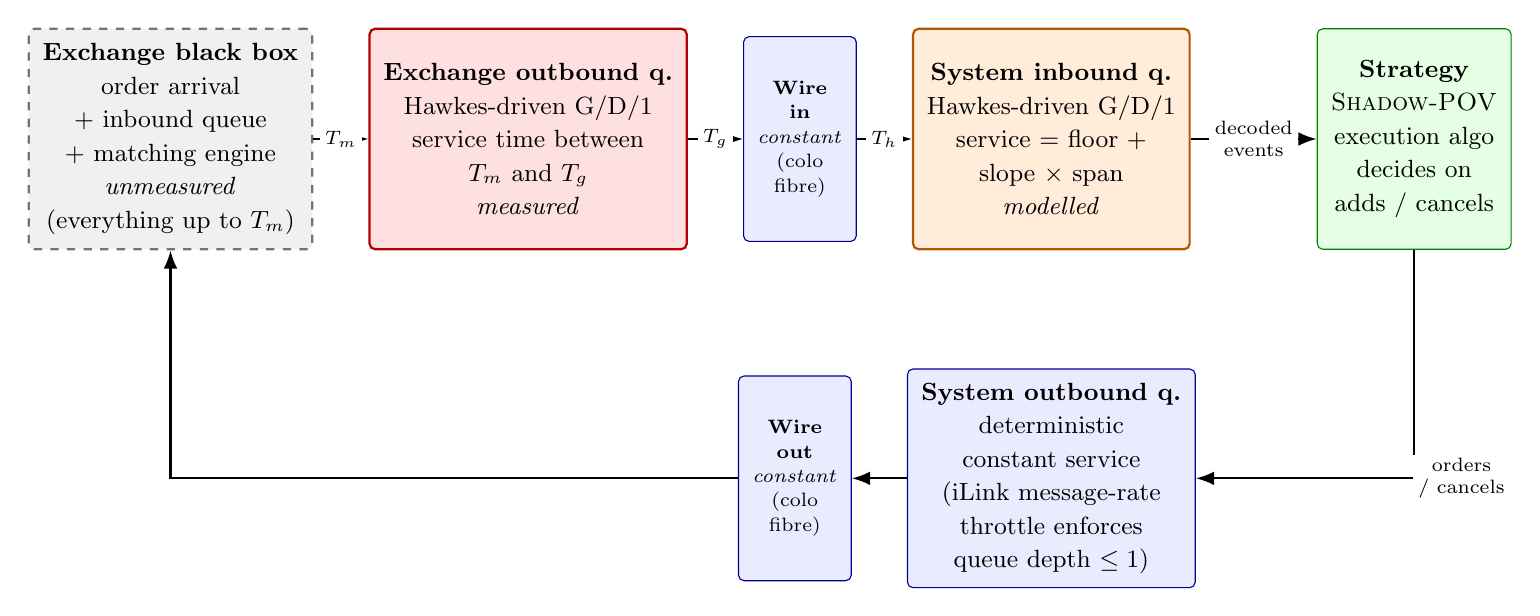
\begin{tikzpicture}[
    node distance=5mm and 7mm,
    box/.style={draw, rounded corners=2pt, minimum height=26mm, minimum width=32mm,
                align=center, font=\small\linespread{1.1}\selectfont, inner sep=5pt},
    blackbox/.style={box, fill=gray!12, draw=black!55, dashed, thick,
                     minimum width=36mm, minimum height=28mm},
    hawkes_meas/.style={box, fill=red!12,    draw=red!70!black, thick, minimum height=28mm},
    hawkes_mod/.style={box,  fill=orange!15, draw=orange!70!black, thick, minimum height=28mm},
    constant/.style={box,    fill=blue!8,    draw=blue!60!black, minimum height=26mm},
    wire/.style={box, fill=blue!8, draw=blue!60!black, minimum width=11mm, minimum height=26mm, font=\scriptsize\linespread{1.1}\selectfont},
    strat/.style={box,       fill=green!10,  draw=green!50!black, minimum width=24mm, minimum height=28mm},
    ar/.style={-Latex, thick},
    lbl/.style={font=\scriptsize, midway, align=center, inner sep=2pt, fill=white, inner ysep=1pt},
]
% Top row (data path, left to right, from exchange to strategy).
\node[blackbox]                                       (ex_bb)    {\textbf{Exchange black box}\\order arrival\\$+$ inbound queue\\$+$ matching engine\\\emph{unmeasured}\\(everything up to $T_m$)};
\node[hawkes_meas, right=of ex_bb]                    (ex_out)   {\textbf{Exchange outbound q.}\\Hawkes-driven G/D/1\\service time between\\$T_m$ and $T_g$\\\emph{measured}};
\node[wire, right=of ex_out]                          (wire_in)  {\textbf{Wire}\\\textbf{in}\\\emph{constant}\\(colo\\fibre)};
\node[hawkes_mod, right=of wire_in]                   (sys_in)   {\textbf{System inbound q.}\\Hawkes-driven G/D/1\\service $=$ floor $+$\\slope $\times$ span\\\emph{modelled}};
\node[strat, right=16mm of sys_in]                    (str)      {\textbf{Strategy}\\\shadowpov{}\\execution algo\\decides on\\adds / cancels};

% Bottom row (order path, right to left, closing the loop).
\node[constant, below=15mm of sys_in]                 (sys_out)  {\textbf{System outbound q.}\\deterministic\\constant service\\(iLink message-rate\\throttle enforces\\queue depth $\leq 1$)};
\node[wire, left=of sys_out]                          (wire_out) {\textbf{Wire}\\\textbf{out}\\\emph{constant}\\(colo\\fibre)};

% Data path (top).
\draw[ar] (ex_bb) -- node[lbl]{$T_m$} (ex_out);
\draw[ar] (ex_out) -- node[lbl]{$T_g$} (wire_in);
\draw[ar] (wire_in) -- node[lbl]{$T_h$} (sys_in);
\draw[ar] (sys_in) -- node[lbl]{decoded\\events} (str);
% Order path (bottom, right to left, closes back into the exchange black box).
\draw[ar] (str.south) |- node[lbl, xshift=6mm]{orders\\/ cancels} (sys_out.east);
\draw[ar] (sys_out) -- (wire_out);
\draw[ar] (wire_out.west) -| (ex_bb.south);
\end{tikzpicture}%
}
\caption{Latency-modelling topology adopted by the paper. Everything up to the matching timestamp $T_m$ --- client-order arrival at the exchange, the exchange inbound queue, and the matching engine itself --- sits inside a single unmeasured region on the left (dashed). The exchange outbound queue between matching and gateway dispatch has a Hawkes-driven G/D/1 tail directly measurable on public MDP3 as the interval $T_g - T_m$. Wire transit is a physical constant. The system inbound queue on the participant's side is a second Hawkes-driven G/D/1, modelled with the two-parameter service (floor plus per-message slope) of Section~\ref{sec:queue}, calibrated from \citet{mayeski_actorhft}. On the order path back to matching, the system outbound queue is a deterministic constant under the iLink participation-throttle argument; the exchange inbound half of the loop is inside the unmeasured region on the left and is assumed common-mode across colo participants so priority is preserved. The two Hawkes-driven components on the data path (red and orange) are the load-bearing objects of this paper.}
\label{fig:latency-topology}
\end{figure}

Four derived tapes are produced per session from the raw MDP3 archive:

\begin{itemize}
    \item a per-message tape carrying $(T_m, T_g, T_h)$ for every message;
    \item a fill tape recording every historical passive maker fill with mid-anchored markouts at multiple horizons;
    \item a channel-wide best bid-and-offer change tape;
    \item a per-UDP-packet aggregate tape.
\end{itemize}

\subsection{Per-window panel}
\label{sec:panel}

For each 30-minute window $W$, an exponential Hawkes intensity of the form

\begin{equation}
\label{eq:hawkes}
\lambda(t) \;=\; \mu \;+\; \alpha \sum_{t_i < t} \exp\bigl(-\beta (t - t_i)\bigr),
\end{equation}

is fitted by maximum likelihood on the sequence $\{T_{m,i}\}_{i \in W}$, using the Ogata recursion for the log-intensity term and the closed-form expression for the compensator integral (Appendix~\ref{app:hawkes}). The window panel records the parameters $(\mu, \alpha, \beta)$, the branching ratio $n := \alpha / \beta$, the long-run intensity $\bar\lambda := \mu / (1 - n)$, and a convergence flag.

Three latency tail statistics are recorded per window (Table~\ref{tab:panel}). Each is reported at both a central and a tail quantile, so that shape ratios $p_{99}/p_{50}$ can be computed.

\begin{table}[htbp]
\centering
\caption{Per-window latency tail statistics.}
\label{tab:panel}
\begin{tabularx}{\textwidth}{@{}l X l l@{}}
\toprule
Statistic & Definition & Quantiles & Units \\
\midrule
Matching-engine latency & $T_g - T_m$ & $p_{50}, p_{99}$ & \si{\micro\second} \\
Send-to-handler latency & $T_h - T_g$ & $p_{50}, p_{99}$ & \si{\micro\second} \\
Modelled queue latency & System time of a single-server queue with deterministic service $s$ on the arrival stream $\{T_{h,i}\}$ & $p_{50}, p_{99}$ & \si{\micro\second} \\
\bottomrule
\end{tabularx}
\end{table}

Windows containing fewer than 10\,000 events are excluded, as are windows within $\pm 1$ day of a front-contract roll. The default service time for the modelled queue tail is $s = 7\,\si{\micro\second}$; the sensitivity to $s$ is examined in Section~\ref{sec:queue}.

\subsection{The \texorpdfstring{$5 \times 5$}{5x5} grid on \texorpdfstring{$(\bar\lambda, n)$}{(lambda,n)}}
\label{sec:grid}

Retained windows are indexed by the pair $(\bar\lambda, n)$. Both axes are partitioned into equal-quantile five-bin edges, defining 25 cells. For each cell we report (i) the count of windows falling in it; (ii) for each of the three latency tails, the median across the cell's windows of the window-level $p_{99}$ (the absolute grid); and (iii) for each tail, the median across the cell's windows of the window-level $p_{99}/p_{50}$ (the relative grid). Cells containing fewer than ten windows are reported as missing. Three tails times two grids together with the cell-mass heatmap yield seven figures in the central panel.

\subsection{Pilot values}
\label{sec:pilot}

The panel-build pipeline is running at the time of writing. Numerical values below are from a single pilot session (2025-01-20, seven retained 30-minute windows). Final tables in the submitted version will report corpus-level medians with bootstrap confidence intervals across the full corpus.

\begin{table}[htbp]
\centering
\caption{Pilot session per-window medians (2025-01-20, NQ front month).}
\label{tab:pilot}
\begin{tabular}{@{}lr@{}}
\toprule
Quantity & Value \\
\midrule
Branching ratio $n$ & 0.807 \\
Long-run intensity $\bar\lambda$ (arrivals per second) & 106 \\
$p_{99}$ matching-engine latency & 3.4 ms \\
$p_{99}$ send-to-handler latency & 20 \si{\micro\second} \\
$p_{99}$ modelled queue latency at $s = 7\,\si{\micro\second}$ & 49 \si{\micro\second} \\
\bottomrule
\end{tabular}
\end{table}

Two observations from the pilot session survive to the full corpus if the pilot is representative. First, matching-engine latency at $p_{99}$ exceeds the receiver-side send-to-handler $p_{99}$ by approximately two orders of magnitude. Second, the fitted branching ratio is close to the critical value at which \citet{dawpender2018queues} predict heavy-tailed queue behaviour.

\subsection{Three tails, three characters}
\label{sec:three-tails}

The three measured tails of Table~\ref{tab:panel} have qualitatively different distributions on the full corpus, and the differences are load-bearing for the rest of the paper. Table~\ref{tab:three-tails} summarises the median-cell values across the $5\times 5$ grid of Section~\ref{sec:grid}, taken from the current 230-session corpus panel.

\begin{table}[htbp]
\centering
\caption{Character of the three latency tails on the $5 \times 5 (\bar\lambda_{\mathrm{pkt}}, n_{\mathrm{pkt}})$ grid, 230-session corpus panel, CME NQ front month. Cell entries are ranges across the 25 grid cells; ``regime span'' is the ratio of the high-corner to the low-corner cell.}
\label{tab:three-tails}
\begin{tabularx}{\textwidth}{@{}l r r r X@{}}
\toprule
Tail & $p_{50}$ range & $p_{99}$ range & $p_{99}/p_{50}$ range & Regime span of $p_{99}$ \\
\midrule
Matching-engine $T_g - T_m$ & ${\approx}90\,\si{\micro\second}$ & $2\,540$--$4\,631\,\si{\micro\second}$ & $27$--$38$ & $\approx 1.85\times$ (monotone in $\bar\lambda$ and $n$) \\
Send-to-handler $T_h - T_g$ & $11$--$12\,\si{\micro\second}$ & $17.1$--$18.6\,\si{\micro\second}$ & $1.50$--$1.61$ & $\approx 1.03\times$ (flat) \\
Modelled queue at $s = 7\,\si{\micro\second}$ & $\approx s$ & --- & --- & --- (see Section~\ref{sec:theory}) \\
\bottomrule
\end{tabularx}
\end{table}

Three characters emerge:

\begin{description}
\item[Matching-engine tail is heavy and regime-conditioned.] The empirical distribution of $T_g - T_m$ has $p_{99}/p_{50} \approx 27$--$38$ across the grid, with the ratio and the absolute $p_{99}$ both increasing with $\bar\lambda$ and with $n$. This is the signature of a queue running near capacity: the median is set by the fast path through the matching engine and gateway, and the tail is set by burst-driven backlog at those stages. The regime-conditioned amplification is the paper's first empirical result. It is not something we model into being --- it is measurable directly from public MDP3 timestamps, and any simulator whose per-message release rule is constant, i.i.d., or a bare draw from an empirical distribution unconditional on the arrival state cannot reproduce it. As noted in Section~\ref{sec:corpus}, $T_g - T_m$ is only the exchange's \emph{outbound} half; a comparable and unmeasured \emph{inbound} queue precedes matching. Under the working assumption that the two halves are of similar magnitude, the exchange service that a client order actually experiences is on the order of twice the numbers reported here, but the shape and regime-conditioning of the distribution --- which is what the modelling depends on --- are argued to be the same on both halves.

\item[Send-to-handler tail is near-deterministic.] The empirical distribution of $T_h - T_g$ has $p_{99}/p_{50} \approx 1.5$ everywhere on the grid, and $p_{99}$ moves by less than $9\%$ from the quiet corner to the busy corner. Given the microstructure of this stage --- one UDP packet from the CME gateway to the receiver's decoder, decoded and stamped inline by \kasparhft{} \citep{mayeski_actorhft} --- this is expected: the receiver-side decoder services one packet at a time and, at production packet rates, the decoder queue is idle far more often than it is busy. The receiver-side queue is a real queue but is not near capacity.

\item[Modelled queue tail is the system queue --- where HFT traders compete.] The modelled queue tail (Section~\ref{sec:queue}) is a synthetic quantity: a Lindley recursion applied to the observed arrival stream with a chosen service time $s$. It is dwarfed in absolute magnitude by the exchange tail --- receiver-side service is in single-digit microseconds against the exchange's milliseconds --- but it is the tail on which high-frequency market participants directly compete. Every HFT participant sees the same exchange latency for a given event; what differs across participants is the microseconds spent on their own side of the wire, between an incoming market-data update and the outgoing add or cancel it induces. Being the first participant with the add, or the first with the cancel, is the entire competitive edge of the trading application, and that edge is bought or lost inside this queue. The exchange service time is fixed by CME; the system-side service time is fixed by the operator's implementation, and every microsecond spent there is a microsecond of information staleness that the strategy's next action must accept. Modelling this queue realistically is therefore central to any HFT backtest of an execution or market-making algorithm, not an incidental correction, and designing the system so that its tail is short --- not merely its median --- is the load-bearing engineering activity for a competitive HFT operator. This is the tail the paper's simulator upgrade of Section~\ref{sec:upgrade} makes contingent on the arrival state rather than on a scalar constant; it is also the tail whose parametric shape is calibrated below from \citet{mayeski_actorhft}. Its character depends on how $s$ is set: at $s$ per message with same-\emph{ns} packet stacking, it inherits the packet-layer discreteness; under a two-parameter service (floor plus per-message slope) calibrated from \citet{mayeski_actorhft}, it recovers a tail close to the receiver-side character of $T_h - T_g$. Section~\ref{sec:queue} treats both cases.
\end{description}

The two empirical tails on the same tape thus have opposite characters: one heavy and regime-conditioned, the other tight and flat. The theoretical section that follows uses this contrast to show which of the standard latency models in Table~\ref{tab:simulators} can reproduce which character, and specifically that only a Hawkes-driven queue near capacity produces the character of $T_g - T_m$.

\section{Data-generation and estimation pipeline}
\label{sec:pipeline}

Every numerical result in this paper is produced by a single pipeline: raw MDP3 records $\rightarrow$ derived message tape $\rightarrow$ per-window Hawkes fit $\rightarrow$ modelled queue tail $\rightarrow$ per-cell grid. This section describes each stage in enough detail for an external reader to reproduce the tables and figures from public data. All code released with the paper is MIT licensed; the software components referenced below are grouped in the companion repository under two names, \texttt{kaspar-hft} (the C++20 replay stack) and \texttt{kaspar\_arrival} (the Python analysis package), whose paths are collected in Appendix~\ref{app:code}.

\subsection{Raw data source and access}
\label{sec:pipeline-data}

The corpus is the historical CME MDP3 feed for channel~318 (NQ E-mini futures) delivered by Databento as per-day pre-decoded binary files. Each file contains one record per SBE message, with the three timestamps $(T_m, T_g, T_h)$ populated directly from the raw feed. Access to CME MDP3 is a paid subscription; the pre-decoded files used here can be obtained from Databento by anyone with a subscription, and the file schema is documented publicly by the vendor. All processing downstream of the raw files is deterministic given the file bytes, so a reader with independent access to the same days will reproduce the tables to the last digit.

\subsection{\kasparhft{} replay stack}
\label{sec:pipeline-kaspar}

\kasparhft{} \citep{mayeski_actorhft} is a discrete-event MDP3 replay simulator built on an actor-model execution framework. In the framework, all in-process components exchange typed messages; the framework guarantees single-threaded processing per actor and a total order across messages consumed by any one actor. Applied to market-data replay, this yields a deterministic pipeline: the same input tape and the same actor graph produce byte-identical output on any host.

The relevant subset of the actor graph for this paper is
\[
\text{PCAP / .bin reader} \longrightarrow \text{MDP3 SBE decoder} \longrightarrow \text{order-book actor (OB)} \longrightarrow \text{recorder actors}.
\]
The reader emits one message per SBE record together with the three raw timestamps. The decoder normalises the record into a typed C++ struct. The order-book actor maintains the market-by-price (or market-by-order) book, updating it deterministically from every incoming message. Recorder actors emit derived tapes: the per-message tape (one row per SBE message, columns $T_m, T_g, T_h$, message kind, side, price ticks, size, and packet coordinates), the best-bid-and-offer change tape (one row per top-of-book change, used to align markouts and to compute mid-anchored quantities), the per-fill tape (Section~\ref{sec:corpus}), and the per-UDP-packet tape (one row per packet, derived by grouping the message tape on $T_g$).

The two recorder driver binaries used to produce the corpus tapes are \texttt{msgtape} (for the message and packet tapes) and \texttt{bin\_replay\_bbo} (for the best-bid-and-offer change tape and the fill tape). Both are single-threaded processes that read one day's pre-decoded file and emit one day's derived tapes. A shell driver script (Appendix~\ref{app:code}) runs the two binaries across the corpus in parallel on 72 cores; per-session determinism means the outer parallelism is embarrassingly parallel with no cross-session state.

\subsection{Per-window panel builder}
\label{sec:pipeline-panel}

The panel builder is a Python program that reads one session's message tape, partitions it into fixed-length windows of length $\Delta = 30\,\text{min}$ aligned to Regular Trading Hours, and emits one row per surviving window into a per-session Parquet file. Windows with fewer than the minimum event count (default $10\,000$) or within one calendar day of a front-contract roll are dropped before Hawkes estimation. The full-corpus panel is the concatenation of the per-session files.

Within each surviving window the builder computes four quantities. First, the empirical distribution of $T_g - T_m$ and $T_h - T_g$ from the window's messages, reported at $p_{50}$ and $p_{99}$. Second, the fitted parameters of an exponential-kernel Hawkes intensity (Section~\ref{sec:pipeline-hawkes}). Third, the modelled queue-latency tail (Section~\ref{sec:pipeline-qsim}). Fourth, a convergence flag from the Hawkes optimisation.

The per-session builder is invoked from the command line with the message-tape path, the output Parquet path, the window length, and the minimum event count. A companion shell driver runs one instance per session in parallel across the corpus; because each session is independent, the outer parallelism is again embarrassingly parallel.

\subsection{Exponential-Hawkes MLE}
\label{sec:pipeline-hawkes}

For a window $W$ containing arrivals $\{t_i\}_{i=1}^{N_W}$ inside an interval $[0, T_W]$ (times measured relative to the window start), the log-likelihood of the exponential-Hawkes intensity of equation~\eqref{eq:hawkes} is
\[
\ell(\mu, \alpha, \beta) \;=\; \sum_{i=1}^{N_W} \log \lambda(t_i) \;-\; \int_0^{T_W} \lambda(u)\, du.
\]
The first term is evaluated by the standard Ogata recursion, which reduces the inner exponential sum to a single running scalar $R_i := \sum_{j < i} \exp(-\beta(t_i - t_j))$ satisfying $R_i = \exp(-\beta(t_i - t_{i-1}))(R_{i-1} + 1)$, so $\lambda(t_i) = \mu + \alpha R_i$; this evaluation is $\mathcal{O}(N_W)$. The compensator integral admits a closed-form expression in $(\mu, \alpha, \beta)$ and in the sequence $\{t_i\}$, given in Appendix~\ref{app:hawkes}. The negative log-likelihood is minimised by L-BFGS-B (SciPy \texttt{scipy.optimize.minimize} with box constraints $\mu > 0$, $\alpha > 0$, $\beta > 0$). Warm starts are used across successive windows of the same session. Windows for which the optimiser fails to converge, or which return a super-critical estimate $\hat n \geq 1$, are marked and dropped. Reported parameters are the branching ratio $\hat n = \hat\alpha / \hat\beta$ and the long-run intensity $\bar{\hat\lambda} = \hat\mu / (1 - \hat n)$.

Estimation is offline in the present paper: the batch fit runs once per new corpus release. The online-fit variant, in which $(\hat\mu, \hat\alpha, \hat\beta)$ are updated recursively from the incoming market-data stream inside the live \kasparhft{} process and consumed by an execution algorithm on the same host, is on the roadmap and is discussed as concrete future work in Section~\ref{sec:future}.

\subsection{Python queue simulation for the panel}
\label{sec:pipeline-qsim}

The modelled queue-latency tail reported in the panel is not a measurement; it is the output of a G/D/1 Lindley recursion applied inside the window to the receiver-side arrival stream $\{T_{h,i}\}$ with a fixed deterministic service time $s$. For each retained window the builder computes the sequence of departure times by equation~\eqref{eq:lindley-d}, and reports the empirical $p_{50}$ and $p_{99}$ of the per-message system time $d_i - T_{h,i}$. The default service time is $s = 7\,\si{\micro\second}$; the sensitivity to $s$ is examined in Section~\ref{sec:queue-sweep}. The Python queue simulation is a numpy scan of length $N_W$ per window and is negligible in runtime compared to the Hawkes MLE.

The same recursion is implemented in C++ inside the \kasparhft{} simulator (Section~\ref{sec:upgrade}) and is exercised on the same tape end to end. The Python implementation exists only for the measurement pipeline; the C++ implementation exists only for the simulator upgrade. Section~\ref{sec:queue-identity} makes this distinction explicit.

\subsection{Grid aggregation and figure production}
\label{sec:pipeline-grid}

The corpus-level grid of Section~\ref{sec:grid} is produced by a small aggregator that reads the per-session panels, applies the equal-quantile binning on $(\bar\lambda, n)$, and writes per-cell medians of the seven quantities of interest (three tails at $p_{99}$, three tails at $p_{99}/p_{50}$, and cell mass). Heatmap figures and the tables reported in the body are generated by a Python plotting script that reads the grid Parquet and emits vector PDF files consumed directly by the \LaTeX{} source of this paper.

\subsection{Reproducibility}
\label{sec:pipeline-repro}

The complete pipeline from raw pre-decoded MDP3 files to the paper's tables and figures is:
\begin{enumerate}
    \item Obtain the Databento pre-decoded MDP3 files for channel~318 over the target date range.
    \item Build \kasparhft{} from source (Appendix~\ref{app:code}); this requires a C++20 toolchain and the CME SBE templates, which are generated by the build.
    \item For each session in the corpus, run \texttt{msgtape} and \texttt{bin\_replay\_bbo} on the corresponding \texttt{.bin} file to produce the four per-session tapes.
    \item Install the \texttt{kaspar\_arrival} Python package (single-file install; requires NumPy, SciPy, Pandas, PyArrow).
    \item Run the batch panel builder across the message tapes to produce the per-window panel Parquet.
    \item Run the grid aggregator to produce the per-cell medians.
    \item Run the plotting script to produce the paper's figures.
\end{enumerate}
Each step above is deterministic in its inputs; there are no random seeds and no timezone-dependent branches. The \kasparhft{} version and the \texttt{kaspar\_arrival} version used to produce a given release of the paper are pinned in the companion repository at the tag corresponding to that release.

\section{A queueing model of exchange- and system-side latency}
\label{sec:queue}

\subsection{Why not Poisson}
\label{sec:notpoisson}

A homogeneous Poisson process is the simplest and most widely used model of an event stream. Its inter-arrival times are exponentially distributed with a single scalar rate, and consecutive arrivals are independent. If MDP3 message arrivals were Poisson, per-window inter-arrival distributions would collapse to a single exponential, autocorrelation of counts across sub-windows would vanish, and any downstream single-server queue would exhibit the closed-form light-tailed behaviour of the M/D/1 or M/M/1 system.

Empirically on CME MDP3 none of these hold. Inter-arrival distributions are strongly heavy-tailed relative to exponential, autocorrelation of counts is positive at all sub-window scales up to the width of the fitting window, and short bursts of arrivals concentrated in intervals of a few microseconds are followed by longer quiet periods. The two-sided departure from a Poisson process motivates a self-exciting alternative.

A Hawkes process \citep{hawkes1971spectra} generalises the Poisson process by making the instantaneous arrival intensity depend on the recent history of events:

\begin{equation}
\label{eq:hawkesgeneral}
\lambda(t) \;=\; \mu \;+\; \int_{-\infty}^{t} \phi(t - u) \, dN(u),
\end{equation}

where $\mu > 0$ is the baseline intensity, $N$ is the counting process of arrivals, and $\phi: (0, \infty) \to [0, \infty)$ is a non-negative memory kernel. Every past arrival contributes a decaying excitation to the current intensity, so a cluster of recent arrivals raises the intensity for future arrivals. The special case $\phi \equiv 0$ recovers the Poisson process. The exponential-kernel choice $\phi(u) = \alpha e^{-\beta u}$ used throughout this paper admits an $O(N)$ recursion for the log-likelihood and the compensator, and the resulting branching ratio $n := \alpha/\beta$ is a scalar summary of the fraction of events attributable to self-excitation.

For CME NQ MDP3 the fitted branching ratio $n$ typically sits close to 1 across the trading day (Table~\ref{tab:pilot} reports $n = 0.807$ on the pilot session), indicating a strongly self-exciting arrival process that a Poisson model cannot reproduce.

\subsection{Definitions}
\label{sec:queue-defs}

Let $\{a_i\}_{i \geq 1}$ denote the arrival-time sequence of messages into a single-server first-come-first-served queue with deterministic per-message service time $s > 0$. The departure time $d_i$ and the per-message system time $w_i$ satisfy the Lindley recursion

\begin{equation}
\label{eq:lindley-d}
d_i \;=\; \max(a_i,\, d_{i-1}) \;+\; s,
\end{equation}

\begin{equation}
\label{eq:lindley-w}
w_i \;=\; d_i - a_i \;=\; \max\bigl(0,\, d_{i-1} - a_i\bigr) \;+\; s.
\end{equation}

Equation~\eqref{eq:lindley-w} admits two regimes. When $a_i \geq d_{i-1}$ the server is idle at the $i$-th arrival and $w_i = s$. When $a_i < d_{i-1}$ the server is still busy processing the previous message; the $i$-th message waits and $w_i = d_{i-1} - a_i + s > s$.

\subsection{Heavy tails under Hawkes arrivals}
\label{sec:queue-tails}

Under Hawkes-clustered arrivals with branching ratio $n < 1$, inter-arrival gaps have a heavy-tailed distribution, and clusters of consecutive arrivals separated by gaps shorter than $s$ occur with a heavy-tailed cluster-size distribution \citep{bacry2015review}. Iterating \eqref{eq:lindley-w} over a cluster of $k$ consecutive arrivals in which every inter-arrival gap is strictly smaller than $s$ yields

\begin{equation}
\label{eq:cluster}
w_{i+k-1} \;\approx\; k \cdot s.
\end{equation}

The tail of the per-message system time $w_i$ therefore inherits the tail of the arrival-cluster-size distribution. This is the queue-Hawkes result of \citet{dawpender2018queues}; it underlies the reporting of the modelled-queue tail in Section~\ref{sec:panel} and the \kasparhft{} simulator upgrade of Section~\ref{sec:upgrade}.

\subsection{Empirical service-time sweep}
\label{sec:queue-sweep}

Figure~\ref{fig:sweep} reports the per-message system-time distribution produced by \eqref{eq:lindley-d}--\eqref{eq:lindley-w} on the arrival stream of one session (2025-01-02, 17.3 million messages) over the range $s \in [1, 20]\,\si{\micro\second}$. The numerical values are collected in Table~\ref{tab:sweep}.

\begin{figure}[htbp]
\centering
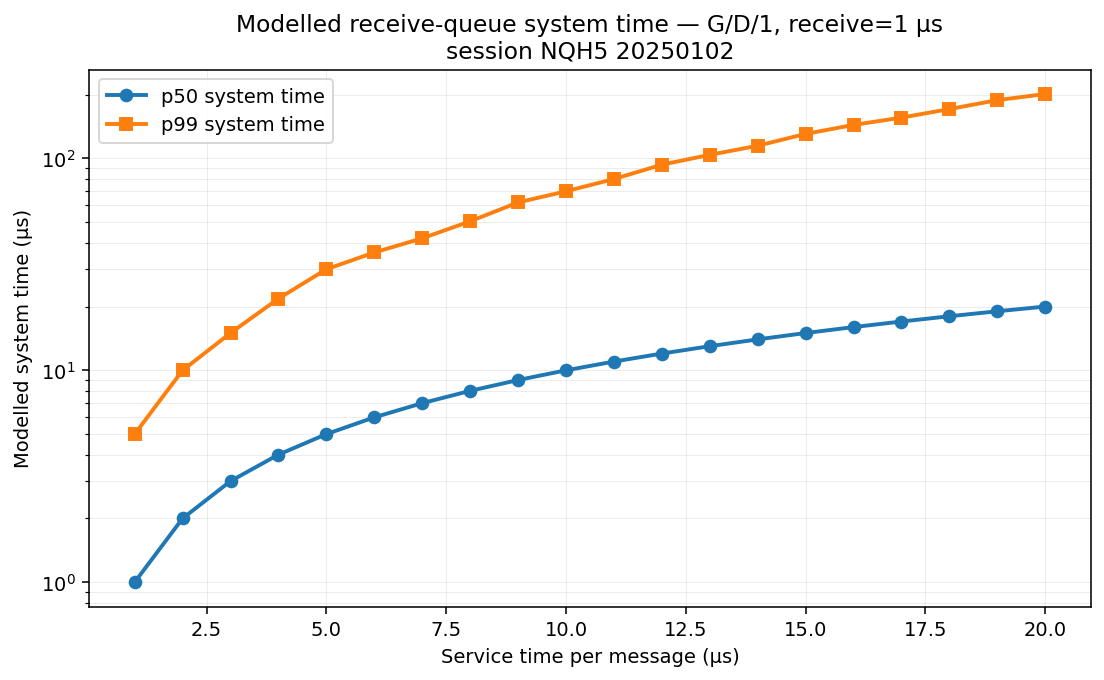
\includegraphics[width=0.85\textwidth]{figs/qlen_service_sweep_20250102.png}
\caption{Modelled per-message system time as a function of deterministic service time $s$, computed by iterating the Lindley recursion \eqref{eq:lindley-d}--\eqref{eq:lindley-w} on the observed handler-end arrival stream of 2025-01-02 (17.3 million messages). Median (blue) tracks $s$ one-to-one; the 99th percentile (orange) grows super-linearly in $s$.}
\label{fig:sweep}
\end{figure}

\begin{table}[htbp]
\centering
\caption{Modelled system time as a function of deterministic service time (one session).}
\label{tab:sweep}
\begin{tabular}{@{}rrrr@{}}
\toprule
$s$ (\si{\micro\second}) & $p_{50}$ (\si{\micro\second}) & $p_{99}$ (\si{\micro\second}) & $p_{99}/s$ \\
\midrule
1  & 1.0  & 5.0   & 5.0 \\
5  & 5.0  & 30.0  & 6.0 \\
7  & 7.0  & 42.0  & 6.0 \\
10 & 10.0 & 70.0  & 7.0 \\
15 & 15.0 & 130.6 & 8.7 \\
20 & 20.0 & 201.5 & 10.1 \\
\bottomrule
\end{tabular}
\end{table}

Two features are visible in the data. First, $p_{50}$ tracks $s$ one-to-one, consistent with the observation that the median arrival meets an idle server. Second, the ratio $p_{99}/s$ grows with $s$, indicating a tail that grows faster than linearly in $s$. As $s$ approaches the median inter-arrival gap on the session (approximately 60 \si{\micro\second}) utilisation $\rho$ approaches unity and the tail diverges in the classical sense; the range of Table~\ref{tab:sweep} lies in the sub-critical regime.

\subsection{Two uses of the same recursion}
\label{sec:queue-identity}

The recursion \eqref{eq:lindley-d}--\eqref{eq:lindley-w} is used in two distinct places in this work, and the distinction between them matters for the argument of the paper.

The first is the \emph{measurement pipeline} of Section~\ref{sec:panel}. There, given a session tape and a chosen scalar service time $s$, we iterate \eqref{eq:lindley-d} once over the observed handler-end stream $\{T_{h,i}\}$ of the session, producing a synthetic per-message system time $w_i$. The empirical $p_{50}$ and $p_{99}$ of $\{w_i\}$ within each 30-minute window are recorded as the modelled-queue tail statistic in the panel. This is a Python analysis of the tape, applied offline once per window.

The second is the \emph{\kasparhft{} simulator upgrade} of Section~\ref{sec:upgrade}. There, the recursion replaces the release rule of the \kasparhft{} simulator's inbound market-data queue and outbound order queue during a simulator run; it drives the timing of every downstream event the \kasparhft{} simulator produces, including fills. This is not a Python analysis of the tape but an in-simulator state machine that generates simulator output.

Both uses of the recursion consume the same arrival sequence and produce identical $w_i$ under identical $s$. Consequently, when the \kasparhft{} simulator is run on the same tape used to build the measurement panel, its per-window $p_{50}$ and $p_{99}$ modelled-queue latencies must match the panel's values to within rounding. This identity is the internal consistency check for the upgrade; a failure of this check invalidates the results reported in Section~\ref{sec:experiment}.

A note on cross-regime dependence, which will be reported once the panel-build pipeline completes. Prior sweeps on individual sessions partitioned into intraday windows (regular hours, FOMC statement, press conference) showed only modest cross-regime differences in $p_{99}$ at fixed $s$, on the order of $20\%$. The full corpus-scale $(\bar\lambda, n)$-conditional analysis of Section~\ref{sec:grid} is the appropriate object for reporting regime dependence and supersedes the illustrative intraday sweep.

\section{\kasparhft{} simulator upgrade}
\label{sec:upgrade}

\subsection{Baseline}
\label{sec:upgrade-baseline}

In its unmodified form the \kasparhft{} simulator, like every discrete-event MDP3 replay simulator surveyed in Table~\ref{tab:simulators}, holds each inbound market-data record for a fixed delay $\delta_{\mathrm{in}}$ and each outbound order for a fixed delay $\delta_{\mathrm{out}}$, releasing them at $a_i + \delta_{\mathrm{in}}$ and $a_i + \delta_{\mathrm{out}}$ respectively. Under this rule the release times are strictly ordered by the arrival times, no message is delayed by any other, and burst-conditioned queue effects are absent.

\subsection{Two-queue upgrade}
\label{sec:upgrade-two-queue}

The proposed upgrade replaces the constant-delay release rule on each side with the Lindley recursion \eqref{eq:lindley-d}--\eqref{eq:lindley-w}. The inbound queue takes market-data records as arrivals and a scalar inbound service time $s_{\mathrm{in}}$; the outbound queue takes simulated orders as arrivals and a scalar outbound service time $s_{\mathrm{out}}$. The two queues operate independently; their release times compose additively into the total simulated round-trip experienced by the algorithm.

The upgrade introduces no new state beyond the two service-time scalars. The \kasparhft{} simulator applies the recursion to the two release queues already present in the constant-delay code path; the change is a single arithmetic edit per queue. A compile-time guard preserves the constant-delay path unchanged; regression tests establish bit-identical output under the guard.

\subsection{Why both inbound delays are kept in the simulator}
\label{sec:upgrade-rationale}

The simulator now carries two Hawkes-driven delay queues on the data path from matching to strategy: the exchange outbound queue (replayed per-message from the observed interval $T_g - T_m$) and the system inbound queue (a G/D/1 Lindley recursion on the participant's side with the floor-plus-slope service of the previous subsection). A reader who has followed the empirical numbers of Section~\ref{sec:three-tails} may reasonably ask why we keep the system-side queue at all: its absolute magnitude, single-digit microseconds, is dwarfed by the exchange outbound tail's several thousand microseconds, and one might expect the strategy's fill outcomes to be governed by the larger of the two.

They are not, and the reason the paper keeps both queues is that they measure two distinct sensitivities of the strategy, informing two distinct engineering decisions:

\begin{description}
\item[Sensitivity to exchange latency.] This is not designable by the operator. It measures how strategy fill rate degrades as the market moves through regimes of higher $\bar\lambda$ and higher $n$ that produce a heavier $T_g - T_m$ tail. The output of this sensitivity is a \emph{strategy-design} decision: whether to widen quotes, reduce participation, or step aside during bursts. It answers ``how much does the strategy have to give back to the market condition itself.''
\item[Sensitivity to own system latency.] This is fully designable by the operator. It measures how strategy fill rate degrades as the participant's own service parameters (floor and slope) get worse. The output of this sensitivity is an \emph{infrastructure} decision: whether the marginal microsecond of engineering effort earns its cost. It answers ``how much does the strategy give back per microsecond of participant-side service.''
\end{description}

The two sensitivities cannot be extracted from a simulator that carries only one queue, because the same fill-rate delta is generated by two independent causes and the two decisions above require them to be separated.

The magnitude comparison sharpens rather than dissolves the case for modelling the system-side queue. The exchange outbound tail is common-mode across every co-located participant on the same instrument: every HFT sees the same $T_g - T_m$ for a given event. What differentiates participants --- and what any competitive market maker or execution algorithm is directly competing on --- is the microseconds spent on their own side of the wire between the incoming market-data update and the outgoing add or cancel it triggers. That differential runs through the system inbound queue and the participant's strategy. Being first with the add, or first with the cancel, is an entirely system-side race, decided within the tail of a queue that this paper is the first to model as Hawkes-driven under a two-parameter service. The system queue is small in absolute terms and load-bearing in relative terms for algorithms whose fill outcomes are decided by such races.

Algorithms differ substantially in how much of their fill outcome depends on such races, and the simulator's two inbound queues make that dependency measurable per algorithm rather than assumed. A percentage-of-volume execution algorithm such as \shadowpov{} decides on \emph{accumulated} volume signals over seconds; passive quotes rest for seconds; a decision to lean more or less aggressive is bought by cumulative deviation from a participation target, not by winning a microsecond race to the touch. For that family we expect a small system-side sensitivity: a change of tens of microseconds in the system inbound service parameters should produce sub-percentage-point changes in fill rate. This is not a limitation of the model; it is a quantitative bound on how much engineering effort a POV-family algorithm can profitably absorb before hitting diminishing returns, and reporting it precisely is the intended output of the sensitivity sweep of Section~\ref{sec:experiment}. Race-sensitive algorithms --- passive market makers with adverse-selection avoidance, latency arbitrage strategies, aggressive taker responders --- would exhibit an order-of-magnitude larger system-side sensitivity on the same simulator, and evaluating them is beyond the scope of this paper but is a direct application of the same tool.

A stronger reason to model the system-side queue explicitly, even when its median contribution is small relative to the exchange, is that the two queues are \emph{in series} on the data path and are driven by the same underlying arrival process. Total per-event latency from matching to strategy is $W_{\mathrm{ex}} + W_{\mathrm{wire}} + W_{\mathrm{sys}}$, and the tails of $W_{\mathrm{ex}}$ and $W_{\mathrm{sys}}$ are not independent random variables that could sum to something intermediate: they are both responses of a Lindley recursion to the same Hawkes-clustered burst, so a burst that inflates $W_{\mathrm{ex}}$ typically also inflates $W_{\mathrm{sys}}$, and the sum compounds rather than averages. What might appear as a system-side latency of a few dozen microseconds in isolation adds to an exchange-side latency of several thousand microseconds during the same burst, and the strategy sees the sum. The magnitude of that compounding, and specifically how much of the joint tail at $p_{99}$ is attributable to each queue, is not computable from either queue's marginal distribution alone; it requires running the simulator with the real span distribution --- because the system-side service under the two-parameter model depends on span, and busy packets are what turn a nominally small system-side floor into a materially larger contribution during the same bursts that inflate the exchange tail. Reporting a per-cell decomposition of the joint $p_{99}$ into the exchange contribution and the system contribution, once the span-conditional service is calibrated, is one of the concrete outputs the paper's simulator upgrade enables.

\subsection{Decomposition of the joint tail}
\label{sec:upgrade-decomposition}

The argument of Section~\ref{sec:upgrade-rationale} makes the modelling choice --- two queues, both Hawkes-driven, in series on the data path --- but it does not by itself demonstrate that both queues contribute measurably to the tail. That demonstration requires an experimental decomposition of the joint $p_{99}$ of per-message end-to-end latency into an exchange-side contribution, a system-side contribution, and a compound term that captures their positive correlation under the same burst. Because the two queues respond to the same underlying arrival process, their contributions are not additive on marginals alone. This subsection specifies two independent decomposition procedures that the panel builder computes per window and per $(\bar\lambda_{\mathrm{pkt}}, n_{\mathrm{pkt}})$ cell, so the two answers can be cross-checked.

For every message $i$ the simulator produces three latency components:
\begin{align*}
w_{\mathrm{ex},i}   &= T_{g,i} - T_{m,i} \quad \text{(measured, per message)}, \\
w_{\mathrm{wire}}  &\equiv w_c \quad \text{(constant, from equal-path colocation)}, \\
w_{\mathrm{sys},i} &= W_{\mathrm{pkt},k(i)} + \text{floor} + \text{slope} \cdot \mathrm{idx}(i)\quad \text{(modelled)},
\end{align*}
where $k(i)$ is the packet containing message $i$, $\mathrm{idx}(i)$ is its zero-indexed position within that packet, and $W_{\mathrm{pkt},k}$ is the packet-level Lindley wait produced by the recursion
$$
D_k = \max(T_{g,k},\, D_{k-1}) + \text{floor} + \text{slope} \cdot (\text{span}_k - 1), \qquad W_{\mathrm{pkt},k} = D_k - T_{g,k} - \text{floor} - \text{slope}\cdot(\text{span}_k - 1),
$$
with floor and slope calibrated per session from a regression of $T_h - T_g$ on within-packet position and overlaid on the fast\_send prior of \citet{mayeski_actorhft}. Total per-message latency is $w_{\mathrm{tot},i} = w_{\mathrm{ex},i} + w_c + w_{\mathrm{sys},i}$.

\paragraph{Method 1 (per-event share).}
For the top $1\%$ of messages by $w_{\mathrm{tot}}$ in the window, take the arithmetic mean of the ratios $w_{\mathrm{ex},i}/w_{\mathrm{tot},i}$ and $w_{\mathrm{sys},i}/w_{\mathrm{tot},i}$. These are the average fractional contributions of each queue among the messages that populate the tail. Fractional attribution; unit-free.

\paragraph{Method 2 (ablation).}
Replace one queue at a time with its median value in the window and re-quantile the totals:
$$
p_{99}^{\text{frozen-ex}}  = Q_{0.99}\!\bigl(\mathrm{median}(w_{\mathrm{ex}}) + w_c + w_{\mathrm{sys}}\bigr), \qquad
p_{99}^{\text{frozen-sys}} = Q_{0.99}\!\bigl(w_{\mathrm{ex}} + w_c + \mathrm{median}(w_{\mathrm{sys}})\bigr).
$$
Then define
$$
\Delta_{\mathrm{ex}} = p_{99}^{\text{full}} - p_{99}^{\text{frozen-ex}}, \quad
\Delta_{\mathrm{sys}} = p_{99}^{\text{full}} - p_{99}^{\text{frozen-sys}}, \quad
\Delta_{\mathrm{cmp}} = \bigl(p_{99}^{\text{full}} - p_{50}^{\text{full}}\bigr) - \Delta_{\mathrm{ex}} - \Delta_{\mathrm{sys}}.
$$
$\Delta_{\mathrm{ex}}$ and $\Delta_{\mathrm{sys}}$ are the tail contributions of each queue in absolute microseconds; $\Delta_{\mathrm{cmp}}$ is the compound term --- the piece of the tail that neither queue alone produces but which appears when both are live because a single arrival-process burst inflates both at once. A non-zero $\Delta_{\mathrm{cmp}}$ is the empirical fingerprint of the correlation argument of Section~\ref{sec:upgrade-rationale}.

The two methods are formalised as Algorithm~\ref{alg:decompose}. Method~1 is a summary over the joint distribution; Method~2 is a controlled counterfactual. Both are cheap: on top of the existing per-window Lindley pass, Method~1 costs one array multiply and a mask, Method~2 costs two extra quantile evaluations. They answer the same question through independent mechanisms, and their agreement is a first-order check that the decomposition is not artefactual.

\paragraph{Span in the simulator: an intentional simplification.}
Algorithm~\ref{alg:decompose}'s expression for $w_{\mathrm{sys},i}$ uses the per-packet span in the service time of the packet-level Lindley recursion, and doing so faithfully would require the simulator to model span as a state-dependent random variable: online estimation of the current $(\bar\lambda, n)$, look-up of the span distribution conditional on that cell, sampling a span per packet, and using that sample in service. The engineering cost is three additional components in the simulator's hot path and a break of the current deterministic-service invariant of Section~\ref{sec:upgrade-two-queue}. The payoff on CME NQ is small: mean span on the corpus is close to unity, span variance is bounded well below its regime-dependent extreme, and the resulting range of packet-service times (from floor at span $= 1$ to floor + slope times a corpus-p99 span of $\lesssim 10$) is much narrower than the Lindley wait itself in the busy cells. The paper's simulator therefore uses a \emph{constant effective service} in the packet-level Lindley,
$$
s_{\mathrm{eff}} = \text{floor} + \text{slope} \cdot \bigl(\bar{\text{span}} - 1\bigr),
$$
where $\bar{\text{span}}$ is the corpus-median span. Span variation is thus absorbed into a single scalar rather than modelled per packet.

This is a stated limitation: the simulator's compound term $\Delta_{\mathrm{cmp}}$ will underestimate the true joint-tail correlation whenever bursts also inflate span, because the span-burst correlation is not carried through the simulator. To keep the reader honest about this, the paper reports the empirical span distribution per $(\bar\lambda_{\mathrm{pkt}}, n_{\mathrm{pkt}})$ cell as a separate figure --- span median, $p_{95}$, and max heatmaps from the panel builder --- so a reader assessing the simulator's fidelity can see directly how much span variation the constant-service simulator averages away. Section~\ref{sec:future-race-algo} lists the state-dependent-span extension as a natural upgrade for future work on race-sensitive algorithms, whose per-message latencies are more sensitive to the extreme high-span packets that this simplification smooths out.

\paragraph{Open question: is span modelling first-order?}
The constant-effective-service simplification described above rests on an untested premise: that the qualitative shape of the modelled tail across the $(\bar\lambda_{\mathrm{pkt}}, n_{\mathrm{pkt}})$ grid is preserved when span variation is replaced by its corpus mean. An earlier version of the panel builder ran the Lindley recursion on individual message arrivals with a fixed per-message service time, and produced a $p_{99}/p_{50}$ ratio that \emph{decreased} with $\bar\lambda$ and $n$ on the corpus grid --- the opposite of the queue-theoretic prediction. That inversion is inconsistent with the paper's central claim that Hawkes-clustered arrivals through a queue produce a regime-conditioned heavy tail, and it is the reason for the packet-level, span-aware service model of Section~\ref{sec:queue}. Two mutually exclusive resolutions are possible:

\begin{enumerate}
    \item \textbf{Span modelling is first-order.} The packet-level Lindley with span-scaled service $s_{\mathrm{eff}}(\text{span}_k) = \text{floor} + \text{slope}\cdot(\text{span}_k - 1)$ produces the physically-expected monotone growth of the modelled $p_{99}/p_{50}$ ratio with $\bar\lambda_{\mathrm{pkt}}$ and $n_{\mathrm{pkt}}$, while the same recursion with span replaced by its corpus mean $\bar{\text{span}}$ retains the inverted gradient. This would mean the simulator must carry a per-packet state-dependent service to reproduce the empirical tail structure at all, not merely to price its magnitude. The constant-effective-service simplification is then untenable, and a state-dependent-span mechanism inside the simulator becomes a required upgrade rather than a stated limitation. This is a strong result: it establishes that the observed regime-conditioning of the receiver-side tail is generated by the joint state-dependence of both packet clustering and span, and reduces every prior single-parameter latency model in Table~\ref{tab:simulators} to a wrong-order approximation.

    \item \textbf{Span modelling is a modest correction.} The packet-level Lindley with span-scaled service and the same recursion with span replaced by $\bar{\text{span}}$ produce quantitatively similar $p_{99}/p_{50}$ grids, both monotone in $\bar\lambda_{\mathrm{pkt}}$ and $n_{\mathrm{pkt}}$; the inversion in the earlier per-message-service version was a specification error at the wrong layer of the pipeline (per-message rather than per-packet arrivals), not a first-order role for span. The constant-effective-service simulator then suffices and the paper's simplification stands.
\end{enumerate}

The paper's empirical resolution of this question --- three grid heatmaps of $p_{99}/p_{50}$ under (a) the per-message-service straw model, (b) packet-level Lindley with constant $s_{\mathrm{eff}}$, and (c) packet-level Lindley with per-packet $s_{\mathrm{eff}}(\text{span}_k)$ --- is a substantive result in its own right and is planned as a subsection of Section~\ref{sec:experiment}. Which of (b) and (c) reproduces the empirical $T_g - T_m$ regime-conditioning at $s_{\mathrm{eff}}$ around the fast\_send calibration is the load-bearing decision for whether the simulator can retain its deterministic-service invariant or must carry a per-packet state-dependent service.

\begin{algorithm}[htbp]
\caption{Per-window decomposition of joint tail latency into exchange and system contributions.}
\label{alg:decompose}
\begin{algorithmic}[1]
\Require Per-message arrays $w_{\mathrm{ex}}$, $w_{\mathrm{sys}}$ (both length $N$), wire constant $w_c$
\Ensure Method~1 shares $\sigma_{\mathrm{ex}}, \sigma_{\mathrm{sys}}$; Method~2 tail contributions $\Delta_{\mathrm{ex}}, \Delta_{\mathrm{sys}}, \Delta_{\mathrm{cmp}}$
\State $w_{\mathrm{tot}} \gets w_{\mathrm{ex}} + w_c + w_{\mathrm{sys}}$
\State $\tau \gets Q_{0.99}(w_{\mathrm{tot}})$; $\mathcal{T} \gets \{i : w_{\mathrm{tot},i} \geq \tau\}$
\State $\sigma_{\mathrm{ex}}  \gets |\mathcal{T}|^{-1} \sum_{i \in \mathcal{T}} w_{\mathrm{ex},i} / w_{\mathrm{tot},i}$
\State $\sigma_{\mathrm{sys}} \gets |\mathcal{T}|^{-1} \sum_{i \in \mathcal{T}} w_{\mathrm{sys},i} / w_{\mathrm{tot},i}$
\State $m_{\mathrm{ex}} \gets \mathrm{median}(w_{\mathrm{ex}})$;\quad $m_{\mathrm{sys}} \gets \mathrm{median}(w_{\mathrm{sys}})$
\State $p_{99} \gets Q_{0.99}(w_{\mathrm{tot}})$;\quad $p_{50} \gets Q_{0.50}(w_{\mathrm{tot}})$
\State $p_{99}^{-\mathrm{ex}}  \gets Q_{0.99}(m_{\mathrm{ex}} + w_c + w_{\mathrm{sys}})$
\State $p_{99}^{-\mathrm{sys}} \gets Q_{0.99}(w_{\mathrm{ex}} + w_c + m_{\mathrm{sys}})$
\State $\Delta_{\mathrm{ex}}  \gets p_{99} - p_{99}^{-\mathrm{ex}}$;\quad $\Delta_{\mathrm{sys}} \gets p_{99} - p_{99}^{-\mathrm{sys}}$
\State $\Delta_{\mathrm{cmp}} \gets (p_{99} - p_{50}) - \Delta_{\mathrm{ex}} - \Delta_{\mathrm{sys}}$
\State \Return $(\sigma_{\mathrm{ex}}, \sigma_{\mathrm{sys}}, \Delta_{\mathrm{ex}}, \Delta_{\mathrm{sys}}, \Delta_{\mathrm{cmp}})$
\end{algorithmic}
\end{algorithm}

The paper reports the results of Algorithm~\ref{alg:decompose} as three heatmaps over the $5\times 5$ $(\bar\lambda_{\mathrm{pkt}}, n_{\mathrm{pkt}})$ grid of Section~\ref{sec:grid} --- median cell values of $\Delta_{\mathrm{ex}}$, $\Delta_{\mathrm{sys}}$, and $\Delta_{\mathrm{cmp}}$ in microseconds --- alongside a scatter of Method~1 shares against Method~2 fractional contributions ($\Delta_j / (\Delta_{\mathrm{ex}} + \Delta_{\mathrm{sys}} + \Delta_{\mathrm{cmp}})$) as the agreement check. The decomposition is what justifies the two-queue simulator upgrade over a single-queue baseline: if $\Delta_{\mathrm{sys}}$ and $\Delta_{\mathrm{cmp}}$ are within the noise of $\Delta_{\mathrm{ex}}$, a single-queue exchange model would recover the tail and the second queue is unnecessary; if they are not, the second queue is doing work that the exchange queue alone cannot, and the paper's simulator upgrade is required.

\subsection{Packet inter-arrival diagnostic}
\label{sec:upgrade-gap-diagnostic}

Before running the three-heatmap experiment above, we run a cheaper first-principle diagnostic that attacks the same question at the arrival process itself. Under a G/D/1 queue with deterministic service $s$, a queue never builds up if the packet inter-arrival gaps $\Delta_k = T_{g,k+1} - T_{g,k}$ almost never fall below $s$: a packet that arrives to an empty server has zero wait and departs after $s$, so a subsequent packet's wait is positive only when $\Delta_k < s$. The diagnostic asks whether packet clustering alone produces such gaps, or whether the queue is only entered when a preceding packet's full span-worth of processing extends past the next packet's arrival.

For each 30-minute window we compute three probabilities:
\begin{align*}
p_{\mathrm{floor}}          &= \Pr\bigl(\Delta < \text{floor}\bigr), \\
p_{\mathrm{mean\text{-}span}} &= \Pr\bigl(\Delta < \text{floor} + \text{slope} \cdot (\bar{\text{span}} - 1)\bigr), \\
p_{p95\text{-}\mathrm{span}}      &= \Pr\bigl(\Delta < \text{floor} + \text{slope} \cdot (\text{span}_{p95} - 1)\bigr),
\end{align*}
where $\bar{\text{span}}$ and $\text{span}_{p95}$ are the mean and $95$th-percentile span in the same window, and floor and slope take the fast\_send calibration values of \citet{mayeski_actorhft}. Aggregated by cell in the $(\bar\lambda_{\mathrm{pkt}}, n_{\mathrm{pkt}})$ grid of Section~\ref{sec:grid}, the three probabilities decode the driver as follows:

\begin{description}
\item[Case A --- packet clustering drives the queue.] $p_{\mathrm{floor}}$ grows with $\bar\lambda_{\mathrm{pkt}}$ and $n_{\mathrm{pkt}}$: packet arrivals cluster tightly enough that gaps below the floor alone are common in busy cells, and the queue builds up without any span assistance. Constant $s_{\mathrm{eff}}$ is sufficient; the simulator's deterministic-service invariant is safe.
\item[Case B --- span drives the queue.] $p_{\mathrm{floor}}$ is uniformly small ($\lesssim 1\%$) across all cells, while $p_{\mathrm{mean\text{-}span}}$ or $p_{p95\text{-}\mathrm{span}}$ grow with $\bar\lambda_{\mathrm{pkt}}$ and $n_{\mathrm{pkt}}$. Packet clustering alone does not queue at the fast\_send floor; queue backlog is generated only when a preceding packet's full processing --- floor plus its span-worth of per-message slope --- extends past the next packet's arrival. The simulator must carry per-packet state-dependent service; the deterministic-service invariant of Section~\ref{sec:upgrade-two-queue} cannot be preserved without paying an accuracy cost in the tail.
\item[Case C --- both contribute.] All three probabilities grow with regime; span and clustering both matter. The constant $s_{\mathrm{eff}}$ simplification is a first-order approximation whose accuracy the three-heatmap experiment above will quantify.
\end{description}

The diagnostic runs as a one-pass groupby on the raw message tape: group by unique $T_g$ per window, take diffs, evaluate the three indicators, average. Runtime is dominated by tape read, not computation, so the corpus-wide diagnostic completes in roughly the same wall-clock as the panel builder itself. The output is one row per window and three heatmaps of the median cell probability, together with per-tail Spearman correlations of each probability against $\bar\lambda_{\mathrm{pkt}}$ and $n_{\mathrm{pkt}}$. Reporting these Spearman coefficients gives a scalar summary of which case the corpus falls into, and the numerical answer directly determines the simulator's chosen service model in Section~\ref{sec:upgrade-two-queue}. This subsection therefore commits the paper to a specific empirical experiment whose outcome fixes a modelling decision that would otherwise remain a subjective simplification.

\subsection{One thread or two: the strategy-actor pipelining question}
\label{sec:upgrade-pipelining}

The topology of Figure~\ref{fig:latency-topology} places the strategy immediately downstream of the system inbound queue, but it does not specify how the strategy's own compute cost enters the latency budget. Two design choices are open to the operator, and this subsection commits the paper to answering which one is correct on measured NQ MDP3.

\paragraph{Choice A --- single-thread fold-in.} The strategy runs on the same thread as the decoder, using \kasparhft{}'s \texttt{fast\_send} \citep{mayeski_actorhft} to invoke the strategy handler inline at the end of each per-message decode step. There is no thread hop, no cross-actor mailbox queue. The effective service time per message becomes $s_{\mathrm{eff}}^{(A)} = \text{floor} + \text{slope} \cdot (\text{span}_k - 1) + s_{\mathrm{strat}}$, where $s_{\mathrm{strat}}$ is the strategy's per-message compute cost, and the paper's existing packet-level Lindley recursion of Section~\ref{sec:upgrade-two-queue} carries the whole latency budget with a slightly enlarged constant.

\paragraph{Choice B --- two-thread pipeline.} The strategy is its own actor on its own thread, with its own inbound mailbox queue. The decoder finishes a message, hands it off through the mailbox (with no \texttt{fast\_send}), and immediately returns to service the next packet. The strategy then processes handed-off messages on its own schedule. Formally, this is a two-stage tandem G/D/1 pipeline: the decoder feeds packets into a stage-1 queue with service $s_{\mathrm{dec}} = \text{floor} + \text{slope} \cdot (\text{span}_k - 1)$; the strategy consumes decoded messages from a stage-2 queue with service $s_{\mathrm{strat}}$ per message. Per-message end-to-end latency is the sum of the stage-1 Lindley wait and the stage-2 Lindley wait, plus the two services.

\paragraph{Practitioner default.} The default choice among HFT practitioners --- documented in industry whitepapers and engineering blogs, but not in the academic literature --- is Choice A: fold work into a single thread and eliminate the cross-thread mailbox handoff. The reasoning is that a thread hop adds cache-line ping-pong, scheduler wake-ups, and cross-core memory-fence cost, on the order of tens to hundreds of nanoseconds per message, and that this overhead outweighs any benefit from splitting the pipeline.

\paragraph{Where the queueing-theory literature already points.} The load-bearing result is a classical asymptotic on tandem queues: the end-to-end delay tail of a stable tandem is dominated by a single stage, not by the sum of stages. Baccelli, Foss and Lelarge \citep{baccellifosslelarge2005} establish it in the general monotone-separable network setting under large deviations: the tandem's end-to-end delay tail has the same asymptotic as the tail of the ``worst'' single stage --- the bottleneck --- and adding a lighter-tailed stage does not change the asymptotic. Foss and Korshunov \citep{fosskorshunov2000} give the corresponding result under heavy-tailed service on feedforward tandems. Daw and Pender \citep{dawpender2018queues}, cited elsewhere in this paper, provide the arrival-process side under Hawkes clustering. Together these results imply that for our two-stage system the end-to-end delay tail is set by
$$
\text{tail}\bigl(w_{\mathrm{end\text{-}to\text{-}end}}^{(B)}\bigr) \;\asymp\; \text{tail}\bigl(w_{\mathrm{single}}(s_{\max})\bigr), \qquad s_{\max} = \max(s_{\mathrm{dec}}, s_{\mathrm{strat}}),
$$
where $w_{\mathrm{single}}(s)$ is the delay of a single G/D/1 queue on the same arrival process with service $s$. The corresponding Choice~A quantity is $w_{\mathrm{single}}(s_{\mathrm{dec}} + s_{\mathrm{strat}})$, on a strictly heavier service. Because Lindley delays grow monotonically in service under a fixed arrival process, this gives a strict theoretical ordering: Choice~B's $p_{99}$ is bounded above by the $p_{99}$ that Choice~A produces, with a gap that widens as $s_{\mathrm{strat}}$ approaches $s_{\mathrm{dec}}$. A concrete illustration for the fast\_send NQ book calibration: at $s_{\mathrm{dec}} = 7.23\,\si{\micro\second}$ and a hypothetical $s_{\mathrm{strat}} = 3\,\si{\micro\second}$, Choice~A's queue runs at service $10.23\,\si{\micro\second}$; Choice~B's asymptotic tail is set by the bottleneck at $7.23\,\si{\micro\second}$; the strategy stage is underloaded and contributes essentially zero to the tail. Multi-stage in the tandem sense \emph{does not add to the tail} beyond its bottleneck asymptotically, and Choice~A's fold-in strictly enlarges that bottleneck.

An important caveat: the tandem $\sim \max$ result is an $x \to \infty$ asymptotic, not a statement about finite quantiles. Foss and Korshunov \citep{fosskorshunov2000} and Baccelli, Foss and Lelarge \citep{baccellifosslelarge2005} prove
$$
P(W_{\mathrm{end\text{-}to\text{-}end}}^{(B)} > x) \;\sim\; \max_j P(W_j > x) \quad \text{as } x \to \infty,
$$
which under light-tailed decay rates $\theta_j$ takes the form $\theta_* = \min_j \theta_j$: the slower-decaying single-stage tail wins the tandem tail asymptotically. At a \emph{finite} quantile such as $p_{99}$, both stages contribute quantitatively and the tandem tail sits between $\max$ and $\mathrm{sum}$:
$$
\max_j\, p_{99}(W_j) \;\leq\; p_{99}\bigl(W_{\mathrm{end\text{-}to\text{-}end}}^{(B)}\bigr) \;\leq\; \sum_j p_{99}(W_j).
$$
How close the finite $p_{99}$ is to $\max$ rather than $\mathrm{sum}$ depends on the gap between the two decay rates, the depth of the quantile (deeper $\to$ closer to $\max$), and the joint dependence structure of the two stage delays under a common Hawkes-clustered arrival process (which the theorems' independence assumption does not carry). Concretely, at $s_{\mathrm{dec}} = 7.23$ and $s_{\mathrm{strat}} = 3\,\si{\micro\second}$, the tandem $p_{99}$ we should expect is not exactly $p_{99}\bigl(W_{\mathrm{single}}(7.23)\bigr)$ but a modest multiple of it; at $p_{999}$ it should be closer to that single-stage $p_{99}$; and at $p_{99999}$ essentially equal. The finite-quantile factor above unity is what the paper's experiment quantifies empirically on the 281-session corpus, at the operationally relevant $p_{99}$.

The gain scales as a clean function of $s_{\mathrm{strat}}$. Because the two service times enter Choice~A additively and Choice~B via the max, the effective-service reduction from A to B is
$$
\Delta s \;=\; (s_{\mathrm{dec}} + s_{\mathrm{strat}}) \;-\; \max(s_{\mathrm{dec}}, s_{\mathrm{strat}}) \;=\; \min(s_{\mathrm{dec}}, s_{\mathrm{strat}}),
$$
a quantity that is zero when either stage has zero cost, maximal when the two stages are balanced ($s_{\mathrm{strat}} \approx s_{\mathrm{dec}}$), and then saturates. Table~\ref{tab:pipeline-gain} tabulates this against representative strategy service times, at $s_{\mathrm{dec}} = 7.23\,\si{\micro\second}$ (fast\_send NQ book floor). Percentage-of-volume algorithms whose per-message compute lands in the $0.5$--$3\,\si{\micro\second}$ band pick up a modest tail reduction; race-sensitive algorithms with heavier per-message logic in the $5$--$20\,\si{\micro\second}$ band pick up an order-of-magnitude larger reduction and are precisely where the tandem architecture matters most (Section~\ref{sec:future-race-algo}).

\begin{table}[htbp]
\centering
\caption{Effective-service reduction from single-stage fold-in (Choice~A) to two-stage tandem pipeline (Choice~B) as a function of strategy per-message service time. Decoder service is held at the fast\_send NQ book floor $s_{\mathrm{dec}} = 7.23\,\si{\micro\second}$. The gain is maximised when strategy service equals decoder service and saturates once the strategy becomes the bottleneck.}
\label{tab:pipeline-gain}
\begin{tabular}{@{}r r r r r@{}}
\toprule
$s_{\mathrm{strat}}$ (\si{\micro\second}) & Choice A eff.\ (\si{\micro\second}) & Choice B eff.\ (\si{\micro\second}) & $\Delta s$ (\si{\micro\second}) & Reduction \\
\midrule
0.5  & 7.73  & 7.23  & 0.50  & 6.5\% \\
1.0  & 8.23  & 7.23  & 1.00  & 12.2\% \\
3.0  & 10.23 & 7.23  & 3.00  & 29.3\% \\
7.0  & 14.23 & 7.23  & 7.00  & 49.2\% \\
10.0 & 17.23 & 10.00 & 7.23  & 42.0\% \\
20.0 & 27.23 & 20.00 & 7.23  & 26.5\% \\
\bottomrule
\end{tabular}
\end{table}

The tandem asymptotic assumes each stage runs on its own server, concurrently. Baccelli-Foss-Lelarge, Foss-Korshunov, and the general monotone-separable framework define feedforward networks in which server~1 processes packet $k$ while server~2 processes packet $k{-}1$; pipelining is intrinsic to the model, not an add-on. Applied to our architecture, Choice~B corresponds to the tandem-queue setting: two threads on two cores, the decoder and the strategy each with their own server. Choice~A does not: it collapses both stages onto a single server with service $s_{\mathrm{dec}} + s_{\mathrm{strat}}$ and is a plain G/G/1, not a tandem. The bottleneck-dominance of the tandem tail is a consequence of the concurrent-server structure, not of the arrival process --- it holds in the theorem's monotone-separable setting precisely because the two stages are separable and run in parallel. Any operator considering Choice~B on a machine with only one core, or on a runtime that pins the two actors to the same core, is running Choice~A regardless of how the code is organised, and none of the results in this subsection apply.

What is missing from the literature is a specific measurement on financial-market microstructure data: the asymptotic ordering is proven in generality but the size of the effect on real CME MDP3 tapes with a specific per-message strategy service is not established.

\paragraph{An honest gap in the literature.} The theoretical anchor of the previous paragraph is a splice of two separate results, not a single theorem, and we state this explicitly because reviewers will look at it. The splice is:

\begin{enumerate}
    \item \textbf{Hawkes drives heavy-tailed single-queue delay.} Daw and Pender \citep{dawpender2018queues} give the asymptotic tail of the workload of a \emph{single} G/D/1 queue whose arrival process is a subcritical exponential Hawkes; the tail is heavier than under Poisson arrivals with the same rate and inherits its shape from the branching-ratio proximity to unity.
    \item \textbf{Heavy-tailed service in tandem is bottleneck-dominated.} Baccelli, Foss and Lelarge \citep{baccellifosslelarge2005}, and Foss and Korshunov \citep{fosskorshunov2000}, give the end-to-end tail asymptotic of a \emph{tandem} feedforward network under \emph{heavy-tailed} service (subexponential or regularly varying), on a general stationary arrival process. The tail is set by one bottleneck stage; adding lighter-tailed stages does not change the asymptotic.
\end{enumerate}

The load-bearing step for our argument is combining the two: a Hawkes-clustered arrival passing through a \emph{tandem} of G/D/1 stages inherits a heavy-tailed effective service via step~1, and the bottleneck-dominance of step~2 then applies. To the best of our knowledge no theorem has been published that closes this chain directly for Hawkes-driven tandem networks --- Daw-Pender treats one queue, and Baccelli-Foss-Lelarge and Foss-Korshunov assume heavy-tailed service on general (not specifically Hawkes) arrivals. The extension is plausible under the same subexponential regularity conditions those results require, but the paper does not prove it, and we do not claim otherwise. Related work that we have surveyed and that does not close the gap either: state-dependent Hawkes queues \citep{gaozhu2024statedep}, Hawkes-driven infinite-server systems \citep{koopsboxmamandjes2018}, delayed Hawkes birth--death processes, and monotone-separable network asymptotics on non-Hawkes arrivals. Closing the Hawkes-driven-tandem asymptotic is a natural follow-on for the queueing-theory literature; it is out of scope for this paper.

\paragraph{The paper's contribution on this point.} We do not claim a new theoretical result and we do not lean on the spliced asymptotic as if it were a theorem. What we contribute is the empirical delta between Choices A and B on the same 281-session CME NQ front-month corpus that carries the rest of the paper, calibrated with the two-parameter service of \citet{mayeski_actorhft} and swept over a plausible range of strategy service times. The measured $p_{99}$ delta, and its scaling with $s_{\mathrm{strat}}$ against $s_{\mathrm{dec}}$, is what an operator making the architecture choice actually needs; it also serves as the empirical corroboration --- on real Hawkes-clustered arrivals --- that the bottleneck-dominance of the general tandem-queue theory carries over to this case. If a reader takes only the numbers and none of the asymptotic argument, the operational recommendation stands.

\paragraph{The tail-versus-median trade-off, and how far splitting goes.} A reader following the argument this far may reasonably ask why the receive pipeline should not be split into arbitrarily many actor stages, since the tandem asymptotic promises a smaller tail with each additional stage. It does not, and the answer is a real design trade-off that the paper's simulator surfaces cleanly rather than obscures.

The mechanism is worth stating precisely, because the intuition is easily misunderstood: splitting does not parallelise the compute of an individual message, only the compute of \emph{different} messages relative to each other. A single message still has to visit every stage in sequence to finish. Take one message with total per-message compute cost $T$ under an empty pipeline. Under a single-stage architecture, that message enters, is worked on for $T$, and exits: end-to-end time $= T$. Under an $N$-stage tandem, that same message enters stage~1, is worked on for $T/N$, is handed off to stage~2 through a mailbox at hop cost $h$, is worked on for $T/N$, is handed off, and so on, exiting after $N$ stage-services plus $N-1$ hops: end-to-end time $= T + (N-1)\cdot h$. The actual work has not decreased; it has been redistributed, and each stage boundary the message crosses is an additive $h$ paid on every message whether the pipeline is busy or idle.

The hop cost $h$ is not itself a constant. Under busy-poll async dispatch between two actors pinned to separate cores using a lock-free MPSC mailbox --- Kaspar-HFT's default configuration --- the hop cost decomposes into three components: sender enqueue ($\sim 10\,\mathrm{ns}$), cache-line transfer between core caches ($\sim 60$--$90\,\mathrm{ns}$), and receiver dequeue ($\sim 10\,\mathrm{ns}$). Median $h \approx 90\,\mathrm{ns}$ under this regime. Occasionally the receiver actor is context-switched off its core --- by an interrupt, a TLB flush, an OS scheduler slice expiry, or a co-hosted actor's activity --- and the next message hop pays a scheduler wake-up on the order of $1$--$3\,\si{\micro\second}$ instead. So $h$ is a random variable with a light-tailed median around $90\,\mathrm{ns}$ and a rare-context-switch tail component in the microsecond band, distinct from the fast\_send paper's $3.4\,\si{\micro\second}$ measurement for the condition-variable async path \citep{mayeski_actorhft} which represents the wait/notify configuration under continuous scheduler wake-up rather than pinned busy-poll. The fast\_send $3.4\,\si{\micro\second}$ figure is plausibly reducible by additional hardening --- spinning receiver threads on pinned cores with interrupt affinity set away, real-time scheduling classes, kernel-bypass IRQ steering --- toward the busy-poll median; fully characterising the hop-cost distribution across dispatch modes and hardening levels is out of scope here and is left for future work on the framework itself (see also Section~\ref{sec:future-race-algo}). For the design analysis below we use the busy-poll median $h \approx 90\,\mathrm{ns}$ and note explicitly where the hop's own tail matters.

Where splitting earns its keep is under \emph{queued} arrivals. Suppose ten messages arrive in a Hawkes cluster too close together for the single-stage server to keep up with. The single-stage server serves them serially, so message~10 exits at $10T$. The two-stage tandem, by contrast, can start message~$k+1$ on stage~1 as soon as stage~1 has finished with message~$k$, in parallel with stage~2 still processing message~$k$; the throughput is $1/(T/2) = 2/T$ rather than $1/T$, and message~10 exits at approximately $5T + T/2 + h$, about half of the single-stage figure. Under an $N$-stage tandem the throughput is $N/T$ and burst exit time falls as $\sim T + (k-1)T/N$. The tail-wait spike above median therefore contracts roughly as $1/N$.

Combining the two effects gives the design equation, to leading order,
$$
\text{median} \;\approx\; T + (N - 1)\cdot h, \qquad \text{tail spike above median} \;\propto\; T/N,
$$
where median rises linearly in $N$ at the small slope $h$ per stage, and tail spike collapses as $1/N$ under a bottleneck-service rate that scales with $N$. Under \texttt{fast\_send}-free async dispatch with $h \approx 90\,\mathrm{ns}$, the median cost of an extra stage is small in absolute terms and the tail win usually dominates; under high-overhead dispatch (blocking mailboxes with wait/notify on 500\,\si{\nano\second}-scale wakeups, or JVM thread-pool dispatch on 1--2\,\si{\micro\second} hops) the median cost swamps the tail win at 2--3 stages already, and there is no benefit to going further.

The remaining practical limit is that work must be \emph{separable} for a split to be even meaningful: SBE decode, book application, strategy signal generation, and order construction form a natural serial chain that admits at most 4--5 clean cut points. Shared-state contention across stages --- locks, atomics on hot data structures, cache-line ownership fights --- which is the classical limit on multi-threaded splitting in threaded C++ or Java code, does not apply under the actor model. By construction each actor owns its state privately, and cross-stage communication is one-way message passing rather than shared reads and writes; the hardware cost of a message hop under \texttt{fast\_send}-free async dispatch is a single cache line moving between cores, which is already priced into the $h \approx 90\,\mathrm{ns}$ constant above. The literature on pipelined systems --- Nginx worker-per-core with per-worker queue, Erlang/OTP actor-per-worker, Aeron/Real Logic feed-handler pipelines, Kafka Streams/Flink operator DAGs --- endorses multi-stage architectures for tail-sensitive workloads but does not endorse unbounded splitting: the number of stages in every one of those systems is bounded by the workload's natural cut points, not chosen to maximise $N$.

For the strategy designer this is a genuine choice, not a decision the tandem theorem resolves. The designer picks the point on the median-vs-tail frontier that matches the algorithm's own sensitivity: a POV-family algorithm that decides on accumulated volume signals prefers small median because absolute latency information staleness matters and its own p99 sensitivity is small (Section~\ref{sec:upgrade-rationale}); a market maker running cancel races against adverse selection prefers small tail because the cost of an occasional lost race dominates. The paper's Choice~B is a two-stage split --- one decoder actor, one strategy actor --- which captures the first-order tandem win and covers the two design points relevant to \shadowpov{}. Whether to split further (SBE decode as its own actor, order construction as its own actor) is an engineering choice bounded by the same trade-off; the paper's simulator supports the extension and Section~\ref{sec:future-race-algo} lists the sweep of $N$ against fixed $T$ as a natural follow-on.

\paragraph{Experimental design.} On the same 281-session corpus and the same top-25\% by daily message volume subset of Section~\ref{sec:experiment-days}, run the packet-level simulator under both architectures at a sweep of strategy service times $s_{\mathrm{strat}} \in \{0.5, 1, 2, 5, 10, 30\}\,\si{\micro\second}$. Choice A uses the paper's existing single-queue Lindley with $s_{\mathrm{eff}}^{(A)}$ as above. Choice B uses a two-stage tandem: stage-1 Lindley on packets with $s_{\mathrm{dec}}$, stage-2 Lindley on messages with $s_{\mathrm{strat}}$, arrivals to stage-2 being the per-message departures from stage-1. All other inputs (arrival stream, calibrated floor/slope, tape) are held identical. For each sweep point and each architecture, report the median-cell $p_{99}$ and $p_{99}/p_{50}$ of per-message end-to-end latency on the $(\bar\lambda_{\mathrm{pkt}}, n_{\mathrm{pkt}})$ grid. The primary chart is $p_{99}^{(A)} - p_{99}^{(B)}$ against $s_{\mathrm{strat}}$: if it is positive and growing in $s_{\mathrm{strat}}$, Choice B (multi-actor pipeline) wins the tail and the wider the strategy service the larger the win.

\paragraph{Scope note.} This subsection commits to the experiment; the numerical result is pending machine time and is reported alongside Section~\ref{sec:experiment}. To simplify the initial modelling, the paper's first version treats the mailbox handoff between stages as a zero-latency dispatch, absorbing the $\approx 90\,\mathrm{ns}$ fast\_send-free hop cost into stage-2's service. A follow-up sensitivity check reintroduces the hop cost and confirms that no plausible hop value changes the direction of the reported result.

\subsection{Conjecture: under Hawkes, the median favours multi-hop}
\label{sec:median-hawkes-conjecture}

The design equation of Section~\ref{sec:upgrade-pipelining} predicts a linear median cost $(N-1)\cdot h$ from $N$-stage pipelining and a $1/N$ tail contraction. Under Poisson arrivals with light load the median is close to the service floor $T$ and the linear-in-$N$ hop term is the only visible effect on the median: the median cost is real and $N$ is bounded by how much of $T$ the operator is willing to pay in hop overhead. Under Hawkes-clustered arrivals the situation may be qualitatively different, because Hawkes bursts inflate the median waiting time at each stage far above the empty-queue floor. We state this as a testable conjecture.

\begin{conjecture}[Hawkes-dominance of the median]
\label{conj:hawkes-median}
Let $W_N^{\mathrm{H}}(\bar\lambda, n)$ denote the median end-to-end latency of an $N$-stage tandem with per-stage deterministic service $T/N + h$ driven by an exponential-Hawkes packet arrival process with mean intensity $\bar\lambda$ and branching ratio $n$, on the paper's calibrated floor and slope. Let $W_N^{\mathrm{P}}(\bar\lambda)$ denote the same tandem driven by a rate-$\bar\lambda$ homogeneous Poisson process (the paper's Poisson null of Section~\ref{sec:notpoisson}). Then on the top-quartile cells of the $(\bar\lambda_{\mathrm{pkt}}, n_{\mathrm{pkt}})$ grid used for the load-bearing sweep,
$$
W_N^{\mathrm{H}}(\bar\lambda, n) \;-\; W_N^{\mathrm{P}}(\bar\lambda) \;\;\gg\;\; (N-1)\cdot h
\qquad\text{for } N \in \{1, 2, 4, 8, 12\},
$$
i.e.\ the Hawkes-versus-Poisson gap in the median at any fixed $N$ is much larger than the entire $N$-stage hop budget. Equivalently, on Hawkes-clustered CME MDP3 arrivals the median end-to-end latency is dominated by cluster-induced queueing at each stage rather than by the constant per-hop cost, and the median penalty of splitting one stage into $N$ is small relative to the median widening the arrival process itself already imposes.
\end{conjecture}

\paragraph{Plausibility argument.} On the paper's calibration, $T \sim 7\,\si{\micro\second}$ and $h \sim 90\,\mathrm{ns}$, so a twelve-stage tandem carries a total hop budget of $\sim 1\,\si{\micro\second}$. Under Poisson at typical operating $\rho$, waiting-time medians of the underlying deterministic-service single-server queue are a small fraction of $T$, and $W_N^{\mathrm{P}} \approx T + (N-1)h$. Under Hawkes at branching $n$ approaching $1$, the queue enters a supercritical-like regime inside clusters even though the long-run $\rho$ is well below one, and the median waiting time inside a cluster is set by the cluster's own duration and packet count rather than by the constant service. Empirically we already observe several-microsecond p50 waits in the top-$n$ cells of the exchange-side tail (Section~\ref{sec:pilot}); if the same regime governs the system side, the median widening from Hawkes vastly exceeds $12 \cdot h = 1\,\si{\micro\second}$. If so, the median-vs-tail Pareto frontier of Section~\ref{sec:upgrade-pipelining} collapses on the median axis: multi-hop pipelining is essentially free on the median and pure win on the tail.

\paragraph{Falsification.} The conjecture is falsified if $W_N^{\mathrm{H}} - W_1^{\mathrm{H}}$ grows at a slope statistically indistinguishable from $h$ per stage on any material subset of the grid, or if the Hawkes-versus-Poisson gap in the median is of the same order as $(N-1)h$ across the grid. Either would restore the median-cost side of the tandem trade-off and would materially constrain how many stages an operator should build.

\paragraph{Experimental design.} The sweep already committed to in Section~\ref{sec:upgrade-pipelining} varies $s_{\mathrm{strat}}$ at fixed $N \in \{1, 2\}$; it does not test the conjecture, which requires a stage-count sweep at fixed $s_{\mathrm{strat}}$. We add the following extension. On the same corpus and the same top-quartile grid cells, run the packet-level simulator at $N \in \{1, 2, 4, 8, 12\}$ tandem stages with per-stage service $T/N + h$ where $T$ is calibrated as in Section~\ref{sec:calibration} and $h = 90\,\mathrm{ns}$ (busy-poll median). For each $N$ report the per-cell $p_{50}$ and $p_{99}$ of end-to-end message latency under (i) the fitted Hawkes arrivals of that cell and (ii) a Poisson null with intensity matched to the same $\bar\lambda_{\mathrm{pkt}}$. Two primary charts:

\begin{itemize}
    \item $p_{50}^{\mathrm{H}}(N) - p_{50}^{\mathrm{P}}(N)$ against $N$, with the $(N-1)\cdot h$ reference line overlaid. The conjecture predicts the Hawkes-Poisson gap sits above this line by at least an order of magnitude across the top-quartile cells; a null result places the gap at or below the reference line.
    \item $p_{99}^{\mathrm{H}}(N)/p_{50}^{\mathrm{H}}(N)$ against $N$, showing the tail-relative-to-median win against pure-median analysis; the conjecture predicts this ratio contracts monotonically in $N$ while $p_{50}^{\mathrm{H}}(N)$ itself moves by less than the hop budget.
\end{itemize}

The hop cost $h$ is treated as a knob in the sensitivity check, sweeping $h \in \{30, 90, 300, 1000\}\,\mathrm{ns}$ so the boundary at which the constant hop overhead becomes comparable to the Hawkes-induced median widening is identified explicitly. This extends the pipelining experiment by one axis ($N$) at moderate incremental cost: the packet-level simulator already runs the two-queue Lindley recursion per window, and the $N$-stage tandem is $N$ sequential recursions on the same input stream.

\paragraph{Positioning against prior art.} The conjecture and its planned empirical test have no direct prior art. The literature closest to it splits along four axes, each of which stops short of the specific claim. On the Hawkes-single-queue side, \citet{dawpender2018queues}, \citet{koopsboxmamandjes2018} and \citet{chenblanchet2021} characterise the waiting-time distribution of a single-server or infinite-server queue driven by Hawkes arrivals but do not compose stages. On the bursty-tandem side, \citet{heindl2001mmpp} and follow-on tandem-decomposition work \citep{kimchydzinski2002mmpp} obtain end-to-end delay moments and percentile bounds for tandem networks under MMPP (Markov-modulated Poisson) input --- bursty but not self-exciting --- and do not decompose the median against a per-hop-cost reference. On the parallel-split side, \citet{gao2024hawkessplit} treat parallel single-server queues fed by randomly split Hawkes arrivals, a different topology whose end-to-end delay is not additive as a series tandem's is. On the datacenter side, \citet{deanbarroso2013tailatscale} and follow-on work on RPC-pipeline tails \citep{zhao2023parsimon} document that per-stage tails compose across stages but treat arrivals as generic bursty and report tail composition rather than a median-vs-stage-count trade-off. The Hawkes-driven series tandem, its median regime under cluster-induced queueing, and the median-vs-$N$ sweep against the $(N-1)h$ reference line are novel to our knowledge. A further differentiator is the empirical calibration: the median widening the conjecture predicts is measured directly on live CME MDP3 PCAP paired with an actor pipeline whose hop cost $h$ is instrumented on the same hardware the simulator runs on, so $T$, $h$ and the Hawkes $(\bar\lambda, n)$ per window come from the same physical stack rather than from assumed distributions. Neither the queueing-theory nor the datacenter literature has access to that combination.

\subsection{Calibration}
\label{sec:upgrade-calibration}

The two service times are supplied by the operator. The inbound service time is obtained by direct profiling of the receive path. The outbound service time is estimated from public MDP3 archives by the procedure of Section~\ref{sec:calibration}.

\subsection{Determinism and cost}
\label{sec:upgrade-determinism}

The recursion is deterministic in market time and produces identical \kasparhft{} simulator output across runs of the same tape with the same service-time parameters. Per-message cost is a single comparison, addition, and assignment.

\section{\shadowpov{} evaluation under flat delay versus tailed delay}
\label{sec:experiment}

Numerical results for this section are pending completion of the measurement pipeline and the \kasparhft{} simulator run. The protocol is fixed below; the corresponding tables and figures will be reported in the submitted version.

\subsection{Algorithm and two evaluation environments}
\label{sec:experiment-design}

The subject of the experiment is \shadowpov{} \citep{mayeski2026shadowpov}, introduced in the Abstract, previously evaluated in the \kasparhft{} simulator under a constant-delay configuration. \shadowpov{} is treated as a fixed black box throughout: its parameters are held constant across every arm of the experiment; only the simulator's per-message latency rule varies.

The experiment is designed to separate two sensitivities of \shadowpov{}'s fill rate that are conflated when a single constant-delay simulator is compared against a single tailed-delay simulator, and to \emph{quantify} both rather than to test a directional hypothesis. Sensitivity (S1): $\partial(\text{fill rate}) / \partial \delta$, where $\delta$ is a constant per-message delay --- how much does the algorithm care about the absolute level of latency. Sensitivity (S2): $\partial(\text{fill rate}) / \partial s$, where $s$ is the system inbound service-time parameter under the two-queue upgrade --- how much does the algorithm care about the microsecond-scale queue behaviour of its own decoder. Under the reasoning of Section~\ref{sec:upgrade-rationale} we expect both to be small for a POV-family algorithm: \shadowpov{} decides on accumulated volume signals rather than winning microsecond races. Reporting these small sensitivities precisely is the intended output; a large sensitivity would be a surprise and would motivate re-designing \shadowpov{} around the arrival-process state, but the a priori expectation is that the numbers land in the low-single-digit percentage-point range across each swept parameter.

\paragraph{Flat-delay sweep.}
The historical constant-delay release rule of the \kasparhft{} simulator is retained, and the per-message inbound-plus-outbound delay $\delta \in \{\delta_1, \delta_2, \dots, \delta_K\}$ is swept across a range spanning approximately two orders of magnitude in the microsecond band relevant to CME colocation ($\delta \in \{10, 30, 100, 300, 1000\}\,\si{\micro\second}$, five points). Every other input to the simulator is held fixed. If \shadowpov{}'s fill rate is a strong function of $\delta$ across this sweep, Hypothesis H1 is supported; if the fill rate curve is nearly flat, H1 is rejected.

\paragraph{Service-time sweep.}
The two-queue G/D/1 release rule of Section~\ref{sec:upgrade} is enabled. The inbound service time is fixed at the operator's directly measured value; the outbound service time $s_{\mathrm{out}} \in \{s_1, s_2, \dots, s_K\}$ is swept across a range covering plausible exchange matching-engine and gateway service times ($s_{\mathrm{out}} \in \{3, 7, 15, 30\}\,\si{\micro\second}$, four points, bracketing the calibrated value of Section~\ref{sec:calibration}). Because the arrival stream is Hawkes-clustered with $n$ close to unity, a small change in $s_{\mathrm{out}}$ translates through the Lindley recursion into a large change in the $p_{99}$ of realised per-order round-trip latency. If \shadowpov{}'s fill rate is a strong function of $s_{\mathrm{out}}$ across this sweep, Hypothesis H2 is supported.

Every sweep point uses identical tape, instrument configuration, algorithm parameters, and random seed. A single collector records posted quotes and fill events at every sweep point. The result is two fill-rate-versus-parameter curves plotted on comparable axes, one against $\delta$ (flat-delay) and one against $s$ (system inbound service-time). Both curves are expected to be relatively flat for \shadowpov{}: for a POV-family algorithm whose decisions are driven by accumulated volume rather than by microsecond races, neither the level of latency nor the microsecond-scale system-queue behaviour materially changes fill outcomes. The non-zero component of the system-side sensitivity comes from the cancel-race sub-loop of the algorithm --- when a burst crosses one side and the algorithm must pull the stale opposite-side quote before the next aggressor arrives, extra system-inbound latency reduces the probability of winning that cancel race. Reporting the two curves precisely quantifies the engineering slack available on this class of algorithm and provides a template that race-sensitive algorithms (market makers with adverse-selection avoidance, latency arbitrage) can apply on the same simulator to obtain their own, expected-larger, sensitivity numbers (Section~\ref{sec:future-race-algo}).

\subsection{Day selection from the grid}
\label{sec:experiment-days}

The mispricing produced by a constant-delay simulator is not uniform across trading days. Latency tails accumulate through the Lindley recursion \eqref{eq:lindley-d}--\eqref{eq:lindley-w} only when inter-arrival gaps become comparable to the service time; on quiet days most gaps are much larger than the service time and the flat-delay and service-time sweeps produce nearly identical fills. The signal is concentrated on days where the arrival process is intense (high $\bar\lambda$) and near-critical (high $n$), because those are precisely the days on which the flat-delay configuration most understates realised latency.

We select the evaluation subset accordingly. From the corpus of approximately 281 sessions in Section~\ref{sec:corpus} we take the top $25\%$ by daily message volume, which yields approximately 70 sessions. The remaining $75\%$ of sessions are held out. The choice is deliberate: fewer sessions carry lower statistical power, but the retained subset is where the two sweeps can plausibly disagree, and averaging over quiet days would dilute the effect the experiment is designed to measure.

The use of daily message volume as the selection proxy relies on a positive rank correlation between daily volume and both $\bar\lambda$ and $n$ within the panel of Section~\ref{sec:panel}. That correlation will be reported explicitly in the final version as a per-session scatter of daily volume against per-session median $\bar\lambda$ and against per-session median $n$, with the corresponding Spearman coefficients. \emph{Pending: this scatter and the associated Spearman coefficients are computed once the panel-build pipeline completes; the top-$25\%$-by-volume subset is fixed by that criterion for the experiment either way.}

\subsection{Reported quantities}
\label{sec:experiment-quantities}

Bootstrap confidence intervals are computed at the session level to prevent intra-session autocorrelation from biasing the standard errors. The primary quantity is fill rate, defined as fills per posted quote, reported at each sweep point in aggregate and per $(\bar\lambda, n)$ grid cell. A secondary quantity is simulated per-order round-trip latency at $p_{50}$ and $p_{99}$, reported at each sweep point to document what the algorithm actually experienced under that configuration. Profit-and-loss and adverse-selection deltas are deliberately not reported: the former conflates the latency effect with the return process on the underlying, and the latter requires a markout distribution whose heavy tails are established prior art \citep{carteajaimungalricci2014} and are not re-measured here. Fill rate isolates the causal effect of the latency configuration while holding the tape, the algorithm, and the seed fixed.

\subsection{Calibration check on order round-trip}
\label{sec:experiment-check}

\emph{Pending. This subsection will report the simulated per-order round-trip latency $p_{50}$ and $p_{99}$ at each sweep point of both sweeps. For the service-time sweep the reported round-trip distribution at each $s_{\mathrm{out}}$ must reproduce the empirical $(\bar\lambda, n)$ grid of Section~\ref{sec:grid} at the corresponding cell for the calibration of Section~\ref{sec:upgrade} to be considered valid; a failure of this check invalidates all downstream results at that sweep point.}

\subsection{Fill rate versus flat delay}
\label{sec:experiment-flat}

\emph{Pending. Table 6 and Figure 3 will report the aggregate fill rate as a function of the flat-delay parameter $\delta \in \{10, 30, 100, 300, 1000\}\,\si{\micro\second}$, with a bootstrap confidence interval resampled by session at each sweep point. Under Hypothesis H1 the curve is a strong function of $\delta$; under its rejection the curve is near-flat across two orders of magnitude in $\delta$.}

\subsection{Fill rate versus service time under the two-queue model}
\label{sec:experiment-service}

\emph{Pending. Table 7 and Figure 4 will report the aggregate fill rate as a function of the outbound service-time parameter $s_{\mathrm{out}} \in \{3, 7, 15, 30\}\,\si{\micro\second}$ under the two-queue Lindley release rule of Section~\ref{sec:upgrade}, with a bootstrap confidence interval resampled by session at each sweep point. The same table breaks the sweep out per $(\bar\lambda, n)$ cell of the grid of Section~\ref{sec:grid}. Under Hypothesis H2 the fill rate is a sharply decreasing function of $s_{\mathrm{out}}$, and the drop is concentrated in high-$\bar\lambda$, high-$n$ cells.}

\subsection{Direct comparison of the two sweeps}
\label{sec:experiment-compare}

\emph{Pending. Figure 5 will plot both curves on a common vertical axis (fill rate) with a shared reference point at the pre-existing operating configuration (flat $\delta = $ historically configured value on one curve; two-queue at the calibrated $s_{\mathrm{out}}$ on the other), and a common horizontal axis of realised $p_{99}$ round-trip latency. A curve that is flat in flat-delay units but sharply decreasing in service-time units at the same $p_{99}$ realised latency is the qualitative shape the experiment is designed to observe.}

\subsection{Interpretation}
\label{sec:experiment-interp}

The experiment is not a new execution algorithm. Its purpose is to separate two hypotheses about \shadowpov{}'s exposure to latency (H1 and H2 of Section~\ref{sec:experiment-design}) that a single constant-delay simulator, or a single tailed-delay simulator, cannot separate. If H1 is supported and H2 is not, the operator's remedy is to add slack in the flat-delay budget; the two-queue upgrade of this paper is not necessary. If H2 is supported and H1 is not --- the outcome anticipated on the basis of the queue theory of Section~\ref{sec:queue-tails} --- the operator's remedy is to reduce the outbound service time (through infrastructure investment) or to condition the algorithm on the arrival-process state that drives it (Section~\ref{sec:future-shadow-design}); adding slack in the flat-delay budget in that case would not help. The value of the reported curves to a practitioner is therefore diagnostic: they identify which of the two remedies is warranted.

\section{Calibration of the exchange service time from public MDP3}
\label{sec:calibration}

The inbound service time $s_{\mathrm{in}}$ is available to the operator by direct measurement of the receive path. The outbound service time $s_{\mathrm{out}}$ is not, since the exchange matching engine is not instrumentable externally. We estimate $s_{\mathrm{out}}$ from public MDP3 archives via the following observation. Under the recursion \eqref{eq:lindley-d}--\eqref{eq:lindley-w} with deterministic service $s$, any arrival that meets an idle server satisfies $w_i = s$. Consequently a low quantile of the empirical distribution of $\{T_{g,i} - T_{m,i}\}_i$ estimates $s$ from below (the estimator is upward biased when no arrival in the corpus meets an idle server, and consistent as corpus size grows in the sub-critical regime).

The estimator is stated formally as Algorithm~\ref{alg:calibrate}.

\begin{algorithm}[htbp]
\caption{Exchange-service-time estimator from public MDP3.}
\label{alg:calibrate}
\begin{algorithmic}[1]
\Require Public MDP3 corpus for the target contract, containing per-message timestamps $\{(T_{m,i}, T_{g,i})\}_{i=1,\dots,N}$; quantile level $q \in (0, 0.05]$ (default $q = 0.01$).
\Ensure Estimated exchange service time $\hat{s}_{\mathrm{out}}$ in microseconds.
\For{$i = 1, \dots, N$}
    \State $\Delta_i \gets T_{g,i} - T_{m,i}$, expressed in microseconds.
\EndFor
\State Discard any $\Delta_i \leq 0$.
\State \Return $\hat{s}_{\mathrm{out}} \gets \mathrm{quantile}_q(\{\Delta_i\})$.
\end{algorithmic}
\end{algorithm}

\paragraph{Optional refinement.} Compute the per-window quantile $\hat{s}_{\mathrm{out}}^{(W)} := \mathrm{quantile}_q(\{\Delta_i : i \in W\})$ for each 30-minute window $W$, and return the corpus mean of $\{\hat{s}_{\mathrm{out}}^{(W)}\}_W$.

A corpus-level estimate on the full NQ corpus is pending. The pilot-session $p_{99}$ of $\{\Delta_i\}$ is 3.4 ms; the corresponding $p_{1}$ is expected to be smaller by several orders of magnitude and to correspond to the effective matching-engine service time.

\section{Discussion and limitations}
\label{sec:discussion}

\subsection{Market impact}
\label{sec:discussion-impact}

The \kasparhft{} simulator contains no market-impact model. Orders submitted by the test algorithm execute against the replayed book without consuming it or triggering a compensating response in the subsequent order flow. Across the sixteen simulators of Table~\ref{tab:simulators}, this places the \kasparhft{} simulator at the passive-replay extreme of a two-family taxonomy of impact treatments.

The first family, present in the agent-based simulators of Table~\ref{tab:simulators} (ABIDES, ABIDES-Markets, MAXE, BSE, DBSE, PyMarketSim, mbt\_gym) and in tape-replay simulators when they permit book-walking (CoinTossX, JAX-LOB, JaxMARL-HFT, StockSharp), models impact mechanically through liquidity consumption and, in the agent-based cases, through endogenous counter-flow generated by the agent population. The realism of the resulting impact is bounded by the calibration of the agent mix.

The second family, appearing in more recent work \citep{noble2026reality,elkarmi2025hawkeslob,berti2025deepmarket,coletta2022cgan}, replaces the agent population with a learned or fitted counter-flow model conditioned on the test agent's actions.

mbt\_gym is the only simulator in Table~\ref{tab:simulators} with an explicit closed-form permanent and temporary impact term (Almgren-Chriss family).

The passive-replay simplification adopted here is defensible for the low-participation regime relevant to the target algorithm; readers evaluating higher-participation strategies should combine one of the surveyed impact models with the two-queue latency upgrade.

\subsection{Other limitations}
\label{sec:discussion-other}

\begin{itemize}
    \item Corpus scope. The measurement corpus is restricted to CME NQ front month. Extension to ES and BTC is left to future work; the calibration procedure of Section~\ref{sec:calibration} generalises but the reported numerical values are NQ-specific.
    \item Interactive fills. Orders submitted by the test algorithm do not perturb the market data; interactive fills that feed back into the arrival process require an agent-based or generative extension (Section~\ref{sec:future}).
    \item Race margin versus per-firm latency. \citet{aquilina2022arms} measure a public race-margin quantity from LSE order-log data. The quantities measured here are per-firm engineering latencies observable in vendor MDP3 archives. The two are distinct and should not be conflated.
    \item Missing pcap timestamps. The vendor pre-decoded archive does not propagate pcap kernel timestamps. Consequently the send-to-handler latency cannot be decomposed into network-transit and software-decode sub-stages. A raw-pcap re-parse would recover this decomposition and permit a sixth measured tail.
    \item Hawkes kernel form. Exponential Hawkes is used throughout for tractability. Power-law kernels \citep{hardiman2013} provide a better fit to the intraday decay curve; adopting them would shift the reported branching-ratio estimates modestly upward without changing the queue recursion or the downstream conclusions.
    \item Deterministic service. The G/D/1 recursion assumes fixed per-message service time. Real decoders exhibit jitter; extending the recursion to G/GI/1 with an additive service-time perturbation is a direct extension.
    \item Substrate. The reference implementation is the \kasparhft{} simulator, a single C++20 discrete-event replay simulator. The recursion is portable to other public simulators (in particular ABIDES) as a single edit to the per-link latency draw, with two additional configuration entries for the inbound and outbound service times. The port is not attempted here.
\end{itemize}

\section{Future work}
\label{sec:future}

\subsection{Implications for \shadowpov{} design}
\label{sec:future-shadow-design}

The experiment of Section~\ref{sec:experiment} evaluates \shadowpov{} with parameters set under a constant-delay configuration of the \kasparhft{} simulator. If the service-time sweep produces a measurable fill-rate degradation while the flat-delay sweep does not --- the outcome anticipated on the basis of the queue theory of Section~\ref{sec:queue-tails}, and concentrated by the setup of Section~\ref{sec:experiment-days} on precisely the days where such degradation is most likely --- the appropriate response in production is not to accept the loss, but to re-design \shadowpov{} so that it is aware of the arrival-process state that drives the extra latency. Concretely, the online Hawkes state $(\bar\lambda, n)$ estimated from the incoming market-data stream should feed \shadowpov{}'s quoting logic: in windows where $\bar\lambda$ and $n$ are both high \shadowpov{} should quote wider on the passive side, reduce participation on the aggressive side, or both, in exact anticipation of the queue backlog that will otherwise degrade fill outcomes.

We do not attempt this redesign in the present paper. Its evaluation would require the tail-aware \kasparhft{} simulator constructed here (a Hawkes-conditioned \shadowpov{} evaluated under constant delay would attribute to the conditioning the effect of throttling during bursts, which a constant-delay simulator does not price), and its parameterisation --- how much wider, at what $(\bar\lambda, n)$ threshold, with what state estimator --- opens a distinct optimisation problem whose merits are best examined in a dedicated study. The empirical building blocks that such a study needs are exactly what the present paper delivers: a per-window state estimator (Section~\ref{sec:panel}), a $5 \times 5$ conditional grid (Section~\ref{sec:grid}), and an evaluation environment in which the state-dependent tail actually manifests (Section~\ref{sec:upgrade}).

\subsection{A concrete follow-on: Hawkes-aware \shadowpov{}}
\label{sec:future-shadow-follow}

A direct follow-on paper would embed a Hawkes-state model inside \shadowpov{} and re-run the experiment of Section~\ref{sec:experiment} with the modified algorithm. Specifically:

\begin{enumerate}
    \item An online $(\bar\lambda, n)$ estimator, evaluated at $O(1)$ cost per market-data event, feeding the algorithm's decision loop.
    \item Participation rate conditioned on the current $(\bar\lambda, n)$ grid cell, throttled in high-$n$ cells and unrestricted in low-$n$ cells.
    \item Passive-quote width conditioned on the cell's expected fill decay.
\end{enumerate}

Evaluation of such a Hawkes-conditioned executor requires the two-queue \kasparhft{} simulator upgrade of Section~\ref{sec:upgrade} as a prerequisite: an evaluation under constant delay would attribute to the Hawkes conditioning the effect of throttling during bursts, which a constant-delay simulator does not price.

\subsection{Evaluation on a race-sensitive algorithm}
\label{sec:future-race-algo}

The system-side sensitivity numbers this paper reports on \shadowpov{} are expected to be small (Sections~\ref{sec:upgrade-rationale} and \ref{sec:experiment}) because a POV-family execution algorithm decides on accumulated volume signals rather than winning microsecond races. \shadowpov{} should nevertheless exhibit a non-zero sensitivity via its cancel-race component during adverse-selection episodes: when a burst crosses one side of a resting quote and the algorithm needs to pull the opposite-side quote before the next aggressor arrives, extra system-inbound latency reduces the probability that the cancel wins. The magnitude of this component is quantified as part of the paper's sensitivity number.

The natural next paper repeats the same two-queue \kasparhft{} evaluation on an algorithm whose fill outcomes are decided \emph{primarily} by microsecond races, so that the tool's discriminative power on the system-side sensitivity can be demonstrated at both ends of the sensitivity spectrum. The candidate is a passive market maker with adverse-selection avoidance --- a strategy family for which the same infrastructure investment that saves negligible fill rate on \shadowpov{} would save order-of-magnitude larger fill rate. Reporting the two sensitivities side by side --- POV-family small, MM-family large --- is the target of that follow-on study.

\subsection{Where the thread-hop cost can be reduced}
\label{sec:future-hopcost}

The trade-off of Section~\ref{sec:upgrade-pipelining} makes clear that the hop cost $h$ is the decisive knob: a smaller $h$ shifts the median-vs-tail Pareto frontier outward and lets more stages be added before the median catches up with the tail win. Under the busy-poll median $h \approx 90\,\mathrm{ns}$ of \citet{mayeski_actorhft}, an $N$-stage tandem carries $(N-1)\cdot 90\,\mathrm{ns}$ of median overhead --- one $\si{\micro\second}$ per twelve stages --- so the median penalty is essentially free relative to a several-microsecond decode floor. Under the fast\_send $3.4\,\si{\micro\second}$ figure for the wait/notify async path the same twelve-stage design would cost $37\,\si{\micro\second}$ of median overhead, several floor-multiples, and no operator would build it.

An honest note on where the levers live. The busy-poll hop between two actor threads has three costs: sender enqueue, cache-line transfer between core caches, receiver dequeue. All three are already in userspace on the same host; the kernel is not on that path, and network-side kernel-bypass data planes such as Solarflare Onload or DPDK do not help --- they reduce the exchange-to-decoder wire path, not the strategy-actor-to-order-router hop. The only lever that belongs to the framework rather than to the operating system is whether the receiver \emph{spins} on its mailbox or \emph{waits} on a condition variable: a spinning receiver is already resident and cache-warm when the sender's write arrives, so there is no scheduler wake-up in the critical path and the hop reduces to a cache-line transfer plus two userspace queue ops. Kaspar-HFT already implements this mode in \texttt{fast\_send}, which is the reason the $90\,\mathrm{ns}$ figure is achievable at all. Beyond that toggle, everything that further reduces $h$ --- forcing Linux to wake the receiver faster, keeping the scheduler from preempting an actor thread, routing NIC and timer interrupts off actor cores, running under a real-time scheduling class, huge pages --- is Linux configuration set by the operator at deployment, not code the framework author writes.

The one framework-side item that is still open, and that we defer to future work, is the design cost of the spinning receiver: a thread that spins on its inbound mailbox pollutes the L1 and L2 caches of its host core, competes with the actor's own working set on that core, and steals memory bandwidth from neighbours. That cost is invisible in the isolated hop-cost microbenchmark but visible in the end-to-end run under realistic load, and it is the reason a framework cannot simply spin every actor by default. The open question is how many stages can be spun before the aggregate cache-pollution cost exceeds the tail-latency win, and whether adaptive spin-then-park heuristics recover the busy-poll floor without the sustained pollution. Characterising that trade-off on realistic HFT workloads, and reporting the resulting achievable number of pipelined actor stages, is the concrete follow-on project. Everything else in the hop-cost budget --- the OS side --- is out of scope for the framework and belongs to an operational-hardening study of the host.

\subsection{Additional extensions}
\label{sec:future-additional}

\begin{itemize}
    \item Cross-product replication on CME ES and CME BTC.
    \item Interactive fills, in which simulated orders feed back into the arrival process.
    \item Port of the two-queue recursion to ABIDES.
    \item Cross-instrument latency coupling (NQ and ES on colocation).
    \item Raw-pcap rebuild to recover network-transit and decoder sub-tails separately.
    \item Extension of the recursion to G/GI/1 with jitter.
    \item Signed-Hawkes directional prediction as a separate research line.
\end{itemize}

\section{Conclusion}
\label{sec:conclusion}

The fill outcomes of an execution algorithm reported by a limit-order-book simulator are only as trustworthy as the simulator's latency model. Sixteen public simulators surveyed in Table~\ref{tab:simulators} model per-message latency as constant, i.i.d., or the emergent behaviour of a real network transport, decoupled from the arrival process. Under the Hawkes-clustered arrival regime of CME NQ MDP3 this decoupling produces a systematic under-representation of tail latency and a corresponding mispricing of strategies whose fills or quote-cancellation behaviour depends on burst-conditioned latency. The paper's simulator upgrade replaces the constant-delay release rule of \kasparhft{} with two Hawkes-driven G/D/1 queues on the data path: the exchange outbound queue whose tail is directly measurable as $T_g - T_m$ on public MDP3, and the participant's own system inbound queue with the two-parameter service (floor plus per-message slope) of \citet{mayeski_actorhft}. Along the order path the system outbound queue is a deterministic constant under the iLink participation-throttle argument and the exchange inbound queue is a priority-preserving common-mode delay under equal-path colocation. The two Hawkes-driven queues measure two distinct sensitivities of the strategy: sensitivity to exchange latency is not designable and informs strategy design during high-$(\bar\lambda, n)$ regimes; sensitivity to system latency is fully designable and quantifies the return on infrastructure investment. Applied to \shadowpov{} \citep{mayeski2026shadowpov}, both sensitivities are expected to be small for a POV-family algorithm, and reporting them precisely places a quantitative bound on how much engineering effort the algorithm can profitably absorb. Race-sensitive algorithms such as passive market makers with adverse-selection avoidance would exhibit an order-of-magnitude larger system-side sensitivity on the same simulator; that evaluation is left for a follow-on study.

\section*{Data and code availability}

The measurement pipeline (message-tape parser, per-window panel builder, calibration script for exchange service time) and the \kasparhft{} simulator with the two-queue upgrade are released with the paper under the MIT licence.

\appendix

% Appendix: Point-process background and estimation reference.
% Pedagogical companion to Sections 2--5 of the main paper.

\section{Point-process background --- every term defined}
\label{app:pp-background}

This appendix builds the vocabulary from scratch. If you already know what a $\sigma$-algebra is you can skim to \S\ref{app:pp-intensity}, but the paper is meant to be readable by people who don't.

\subsection*{Warm-up: the Poisson process in plain English}
\label{app:pp-warmup}

Before defining a ``point process'' formally, meet its simplest member: the Poisson process. Once you're comfortable with this, the rest of the appendix is just formalising it and generalising it.

\paragraph{The setup.} Imagine you're watching messages arrive from a market-data feed and you write down the time of each arrival:

\begin{verbatim}
09:30:00.213    <- 1st arrival
09:30:00.451    <- 2nd
09:30:00.802    <- 3rd
09:30:01.014    <- 4th
09:30:01.317    <- 5th
...
\end{verbatim}

That list of timestamps is the raw thing we're going to model. Nothing else --- no prices, no sides, just when.

\paragraph{The Poisson idea.} Imagine that every very-tiny fraction of a second, there is some \emph{small independent} chance an arrival happens. Independent means: whether one arrives right now doesn't depend on when the previous one came, or how many happened in the last minute, or anything about the past. It's like flipping a huge number of very-biased coins, one for each tiny sliver of time, and calling an arrival every time one comes up heads.

The \emph{rate} of the process is a single number, usually written $\lambda$ (``lambda'', for now think ``rate'') or $\mu$ (``mu''), in units of \emph{arrivals per second}. Concretely, if the rate is 300 per second:
$$\mu = 300\ \text{arrivals per second},$$
then on average you get 300 arrivals per second, forever.

Three consequences that follow purely from ``each tiny sliver is independent'':

\paragraph{(1) The time between consecutive arrivals (``gap'') follows an exponential distribution with mean $1/\mu$.} If $\mu = 300$ per second, the mean gap is
$$\text{mean gap} = \frac{1}{\mu} = \frac{1}{300/\mathrm{s}} \approx 3.3\ \mathrm{ms}.$$
The gap distribution has the memoryless property: no matter how long you've been waiting, the expected time to the next arrival is still 3.3\,ms. The probability the next gap exceeds some time $\Delta$ is
$$\Pr(\text{gap} > \Delta) = e^{-\mu\,\Delta}.$$
Substituting our example rate gives $\Pr(\text{gap} > 3.3\,\mathrm{ms}) \approx 36.8\%$, $\Pr(\text{gap} > 6.6\,\mathrm{ms}) \approx 13.5\%$, $\Pr(\text{gap} > 10\,\mathrm{ms}) \approx 5.0\%$. Conversely, the probability the gap is shorter than one-tenth of the mean is
$$\Pr\!\big(\text{gap} < \tfrac{1}{10}\,\text{mean}\big) = 1 - e^{-0.1} \approx 9.52\%.$$
This $9.52\%$ number appears again in the rest of the paper. It's the Poisson benchmark for ``how often do two arrivals come nearly back-to-back''. If empirical data shows 60--85\% instead of 9.52\%, we've rejected Poisson.

\begin{figure}[H]
    \centering
    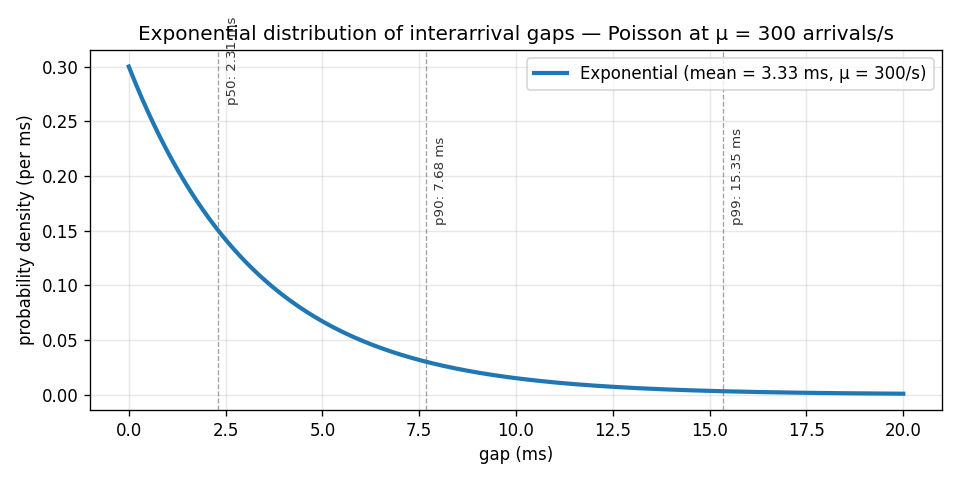
\includegraphics[width=0.75\textwidth]{figs/exponential_gaps.png}
    \caption{The exponential PDF of interarrival gaps for a rate-$300/$s Poisson process. Dashed vertical lines mark the p50 (median), p90, and p99 quantiles. Under Poisson, half the gaps are shorter than the median 2.3\,ms and 10\% are longer than 7.7\,ms --- a specific shape with a soft right tail. Real CME MDP3 data has a completely different shape: far more mass near 0 (bunched arrivals) and a much heavier right tail (long quiet stretches).}
    \label{fig:exponential-gaps}
\end{figure}

\paragraph{(2) The count in any window of length $T$ is Poisson-distributed.} Let $C$ be the count of arrivals in a window of length $T$:
$$\mathrm{E}[C] = \mu T, \qquad \mathrm{Var}[C] = \mu T$$
(same as the mean --- that's the defining property of a Poisson distribution). So the ratio of variance to mean in \emph{any} window $T$ is
$$\frac{\mathrm{Var}[C]}{\mathrm{E}[C]} = 1$$
always. This ratio is called the \textbf{Fano factor} (\S\ref{app:pp-fano} formally defines this); Poisson gives Fano $= 1$ at every window size. Any departure from this is a rejection of Poisson.

\paragraph{(3) The count in disjoint windows is independent.} Whatever happened in $[0, 1\,\mathrm{s}]$ tells you nothing about how many arrivals happen in $[1\,\mathrm{s}, 2\,\mathrm{s}]$. No memory, no clustering, no repulsion --- just independence.

\paragraph{Why Poisson is the ``null hypothesis'' everyone starts from.} Poisson is what happens if arrivals are ``as random as possible'' --- no self-reinforcement, no clustering, no bunching, no memory. It's what a purely mechanical, uncoordinated source would look like. Every departure from Poisson tells us something about the market: bursts of information, coordinated flow, self-reinforcing feedback.

\paragraph{Two ways real market data rejects Poisson.} \emph{Bunching}: real messages arrive in bursts. Many gaps are far shorter than the exponential mean would predict --- in ES/NQ we see 60--85\% of gaps shorter than mean$/10$, versus Poisson's 9.52\%. \emph{Momentum in the intensity}: after a burst starts, more arrivals are likely to keep coming. That's the opposite of Poisson's memoryless assumption. To model these, we need a class of processes that is Poisson-like locally (arrivals still happen randomly on tiny timescales) but where the \emph{rate} itself changes with the history. That's exactly a \textbf{conditional-intensity point process}.

\paragraph{Notational note.} Some authors write the Poisson rate as $\lambda$, others as $\mu$. In this appendix $\mu$ is reserved for the \emph{background} rate of a Hawkes process (which reduces to plain Poisson when the excitation kernel is zero), and $\lambda(t)$ is reserved for the general time-varying conditional intensity. For a plain Poisson process, $\lambda(t) = \mu$ for all $t$.

\subsection{What is a point process and what is a point}
\label{app:pp-pointprocess}

\begin{itemize}
    \item A \textbf{point} here means a single instant in time when something happens. Not a spatial point, not a decimal point. Just one instant --- the timestamp of one message arriving from the CME feed.
    \item A \textbf{process} is a random object that unfolds in time. A coin flipped once is random but static; a stock price ticking through the day is a random \emph{process}. In our case the process produces a random \emph{list of arrival timestamps} $t_1, t_2, t_3, \ldots$
    \item A \textbf{point process} is a random sequence of points (timestamps) on the real line, specified by \emph{when} events happen and nothing else.
\end{itemize}

If each event also carries additional information (side, price, size), that's a \textbf{marked point process} --- the timestamps are the ``points'' and the additional info per event is called a \textbf{mark}. Our arrival streams are naturally marked, but for arrival-process characterisation we mostly ignore the marks and treat only the timestamps as the process.

Alternative names in the literature: ``counting process'' (emphasises $N(t)$), ``temporal point process'' (distinguishes from spatial), ``renewal process'' (a specific subclass --- \S\ref{app:pp-canon}b), ``self-exciting process'' (Hawkes --- \S\ref{app:pp-canon}c).

\paragraph{Concrete example.} Between 09:30:00 and 09:30:01 of NQ March 2025 the following four MBO arrivals occur:
\begin{verbatim}
09:30:00.001234567   Add,    bid 21432.50, size 3
09:30:00.001234571   Add,    ask 21432.75, size 5
09:30:00.017891234   Cancel, order X, bid 21432.25
09:30:00.238491702   Trade,  ask 21432.75, size 2
\end{verbatim}
The point process is just the four timestamps. The marks (Add/Cancel/Trade, side, price, size) are additional per-event data.

\subsection{The setup: a probability space}
\label{app:pp-probspace}

We model market-data arrivals as a \textbf{stochastic process}: a family of random variables indexed by time. The underlying machinery is a probability space $(\Omega, \mathcal{F}, \Pr)$:

\begin{itemize}
    \item $\Omega$ (``sample space'') --- the set of all possible outcomes of the whole experiment. Here an outcome is one specific realisation of the market's day: the complete list of arrival timestamps, prices, sides, etc. You never see $\Omega$ directly; it exists to make everything else well-defined.
    \item $\mathcal{F}$ (``$\sigma$-algebra'') --- think of it as the exhaustive list of yes-or-no questions we're allowed to ask about the outcome and to which a probability can be assigned. Each such question corresponds to a subset of $\Omega$: the subset for which the answer is ``yes''. Two examples: ``did at least one message arrive between 09:30:00 and 09:30:01?'' and ``did the front contract trade above 21500 at some point?'' The two rules a $\sigma$-algebra must satisfy just say the catalog is closed under negation and countable union. Every event you'd naturally think of lives in it. For our timestamp setting, $\mathcal{F}$ is the standard Borel $\sigma$-algebra --- the natural catalog of yes/no questions on the real line.
    \item $\Pr : \mathcal{F} \to [0, 1]$ --- assigns a probability to each event. Satisfies $\Pr(\emptyset) = 0$, $\Pr(\Omega) = 1$, and countable additivity on disjoint events.
\end{itemize}

\subsection{Filtration: how information accumulates over time}
\label{app:pp-filtration}

At time $t = 0$ we know nothing yet. As time passes we observe more arrivals. To formalise this we use a \textbf{filtration}, an increasing family of $\sigma$-algebras:
$$\{\mathcal{F}_t\}_{t \geq 0}, \qquad \mathcal{F}_s \subset \mathcal{F}_t \text{ for } s \leq t.$$
$\mathcal{F}_t$ is the $\sigma$-algebra of everything observable by time $t$ inclusive. $\mathcal{F}_{t^-}$ is everything observable strictly before $t$. When a formula says ``conditional on $\mathcal{F}_{t^-}$'', it means ``given everything we've seen strictly before time $t$''. A process is \emph{adapted} to $\{\mathcal{F}_t\}$ if for every $t$ its value is measurable with respect to $\mathcal{F}_t$ --- i.e., knowable from the history up to $t$.

\subsection{The counting process $N(t)$}
\label{app:pp-counting}

The observable object is a random function of time:
$$N(t) = \#\{\, i : t_i \leq t \,\}.$$
$t_1, t_2, \ldots$ are the (random) arrival times; $N(t)$ is a non-decreasing, right-continuous, step function of $t$ that jumps by 1 at each arrival with $N(0) = 0$. The number of arrivals in a half-open interval is
$$N(t + h) - N(t) = \text{number of arrivals in }(t, t + h].$$

\subsection{Conditional intensity: the current speed of the process}
\label{app:pp-intensity}

\paragraph{Plain English first.} At any moment $t$, ask two questions: (1) ``what's the probability that at least one new message arrives in the next tiny sliver of time, of length $h$ seconds?'' and (2) ``given all the messages we've already seen up until right now (but not including $t$ itself), how does that probability behave as $h$ gets very small?'' The \textbf{conditional intensity} $\lambda(t)$ is the answer to (2), divided by $h$, in the limit as $h \to 0$. It's the instantaneous rate of arrivals at time $t$, conditional on the history. If the current rate is 300 per second, then the chance of an arrival in the next 1 ms is
$$\Pr(\text{arrival in next }1\,\mathrm{ms}) \approx \lambda(t)\, h = 300 \times 0.001 = 30\%.$$

\paragraph{Formula.}
$$\lambda(t \mid \mathcal{F}_{t^-}) = \lim_{h \downarrow 0} \frac{1}{h}\; \Pr\!\big(\, N(t + h) - N(t) \geq 1 \,\big|\, \mathcal{F}_{t^-} \big).$$
Piece by piece: the raw probability inside is ``the probability that at least one new message arrives in the next $h$ seconds, given the entire history strictly before now.'' Dividing by $h$ converts probability to a rate, and the limit as $h \to 0$ gives $\lambda(t)$ in units of arrivals per second.

\paragraph{Contrast with Poisson.} If $\lambda(t) = \mu$ for all $t$ regardless of history, that's Poisson: the conditioning bar carries no information.

\paragraph{Contrast with Hawkes.} In a Hawkes process the intensity is the background $\mu$ \emph{plus} a sum over past arrivals of a decaying excitation contribution $\phi(t - t_i)$:
$$\lambda(t) = \mu + \sum_{t_i < t} \phi(t - t_i).$$
Each past event bumps $\lambda(t)$ up, and the bump decays as time since that event grows.

\paragraph{Useful shortcuts.} For small $h$:
$$\Pr(\text{arrival in }(t, t+h]) \approx \lambda(t)\, h, \qquad \mathrm{E}[N(b) - N(a)] \approx \int_a^b \lambda(s)\, ds.$$
Once we've said what $\lambda(\cdot)$ is as a function of history, we've said everything about the point process.

\subsection{Three canonical models}
\label{app:pp-canon}

\paragraph{(a) Homogeneous Poisson.} $\lambda(t) = \mu$, $\mu > 0$. Gaps between consecutive arrivals are i.i.d.\ exponential with mean $1/\mu$. The count in any window of length $T$ is $\mathrm{Poisson}(\mu T)$ with mean and variance both $\mu T$. Every summary statistic reduces to a triviality: coefficient of variation $\mathrm{CV} = 1$, Fano factor $F(T) = 1$ at every $T$, Hurst exponent $H = 0.5$, gap autocorrelation zero at every lag. This is the null hypothesis every microstructure paper rejects.

\paragraph{(b) Renewal process.} Interarrival gaps $\Delta_i = t_i - t_{i-1}$ are drawn i.i.d.\ from some common distribution $G$, not necessarily exponential. The intensity is a function of time since the last arrival, $\lambda(t) = h(t - t_{\mathrm{last}})$, where $h(\cdot)$ is the hazard function of $G$. Renewal $\neq$ Poisson unless $G$ is exponential. Renewal produces high CV and high Fano at short $T$, but not sustained clustering over time. Shuffling the gap sequence via a Fisher--Yates permutation leaves a renewal process statistically identical. This is why the Fisher--Yates shuffle test (\S\ref{app:diag-order}) separates renewal from Hawkes: under Hawkes the ordering matters; under renewal it doesn't.

\paragraph{(c) Hawkes (self-exciting) process.} Each past arrival transiently raises the intensity:
$$\lambda(t) = \mu + \sum_{t_i < t} \phi(t - t_i).$$
$\mu \geq 0$ is the \textbf{background rate}, the intensity that would exist with zero prior arrivals (news, order flow uncorrelated with prior events). $\phi:(0, \infty) \to [0, \infty)$ is the \textbf{kernel}, or excitation function: given that an arrival happened $u$ seconds ago, $\phi(u)$ is how much extra intensity that arrival still contributes right now. $\phi$ decays: recent arrivals contribute more than old ones.

\emph{What ``kernel'' means in plain English.} The word here has nothing to do with corn or operating systems; it's math jargon for a function that says ``how much a past event still matters at any later time''. Metaphors: (i) ripples in a pond --- drop a stone, it creates a ripple that spreads and fades. If you drop several stones the total disturbance at any moment is the sum of the individual ripples still going, each faded by its own elapsed time. (ii) A bell ringing --- strike the bell, it rings loudly then decays. If someone hits the bell many times, the total sound now is the sum of all past strikes decaying according to time since each strike. In a Hawkes process every past arrival is one such stone drop or bell strike; the intensity now is $\mu$ plus the sum of residual echoes from every past arrival. So the kernel is the shape of one event's future influence. Two properties follow: (1) $\phi$ must decay so that the total area $n = \int \phi$ is finite, otherwise past events would matter forever and the process would build up to infinity; (2) $\phi$ must be non-negative --- a past event can only raise future intensity in a self-exciting model.

\paragraph{Kernel families.} Two standard choices:

\emph{Exponential kernel:} $\phi(u) = \alpha\, e^{-\beta u}$. Two parameters: $\alpha \geq 0$ is the jump size (intensity increment immediately after an arrival), $\beta > 0$ is the decay rate ($1$/time-constant). This is what we fit primarily. Its virtue is \emph{Markovian}: the current intensity summarises all the information needed from the past, so only one running number needs updating when a new event arrives. Concretely, if $\lambda(t)$ is the intensity right before a new event, then right after that event it becomes $\lambda(t) + \alpha$, and between events it decays as $\mu + (\lambda(t) - \mu) e^{-\beta \Delta t}$. Nothing else about the past enters. Intensity updates recursively in $O(1)$ per arrival.

\emph{Power-law kernel:} $\phi(u) = a\,(u + c)^{-(1+p)}$, $p > 0$. Slower decay; consistent with the Hardiman--Bouchaud finding that CME kernels look power-law over long horizons. Considered as a goodness-of-fit follow-up.

\subsection{Branching ratio $n$}
\label{app:pp-branching}

$$n = \int_0^\infty \phi(u)\, du.$$
$n$ is the mean number of direct offspring arrivals that a single arrival triggers. For the exponential kernel $n = \alpha/\beta$, a two-line calculation.

Interpretation as a \textbf{branching process} (or Galton--Watson process, from the 19th-century statisticians who studied surname extinction with it). Every arrival is either exogenous (spawned by $\mu$) or endogenous (a child of some earlier arrival). On average each arrival has $n$ direct children. Expected total cluster size initiated by one exogenous arrival is a geometric series:
$$1 + n + n^2 + n^3 + \cdots = \frac{1}{1 - n} \qquad (n < 1).$$
When $n < 1$ the process is \textbf{subcritical / stationary}: clusters are finite and the long-run stationary rate is $\mu / (1 - n)$. When $n \to 1^-$ the process is \textbf{near-critical}: cluster sizes and durations diverge, long-range dependence appears. When $n \geq 1$ the process is \textbf{supercritical}: with positive probability a single arrival spawns an infinite cascade in finite time, which we do not observe in nature.

Empirically on ES/NQ book feeds the branching ratio sits in a narrow window near 1: $n \approx 0.85$ to $0.97$. That is the ``close to critical'' story from Filimonov--Sornette and Hardiman--Bouchaud that we replicate and extend.

\subsection{Visualising the two knobs}
\label{app:pp-visualise}

Two Hawkes fits with the same branching ratio but different mean intensity look completely different in an event raster, and same-intensity but different-branching fits look completely different too. Since these are the two knobs the paper stratifies by, spend a minute looking at how they trade off visually.

We simulate an exponential Hawkes on a fixed 60-second window at each of nine $(\bar\lambda, n)$ combinations --- the $3\times 3$ factorial of $\bar\lambda \in \{2, 10, 50\}$ events/s and $n \in \{0.30, 0.60, 0.90\}$. For each cell we show: (i) event raster --- every arrival as a vertical tick, revealing visible clustering; (ii) count curve $N(t)$ --- steeper stretches indicate bursts; (iii) intensity trace $\lambda(t)$ --- peaks after clusters, decays during quiet stretches.

\emph{What you should see across the panels.} Low $\bar\lambda$, low $n$ ($\bar\lambda=2$, $n=0.30$) is nearly Poissonian --- ticks uniformly random, count curve straight, intensity flat with tiny wiggles. High $\bar\lambda$, low $n$ ($\bar\lambda=50$, $n=0.30$) is dense but still nearly Poissonian --- ticks packed together but distributed evenly, intensity trace roughly constant. Low $\bar\lambda$, high $n$ ($\bar\lambda=2$, $n=0.90$) is the most instructive: mean rate 2/s but arrivals in unmistakable bursts, long empty stretches punctuated by rapid clusters, intensity spikes to 20--30/s locally. High $\bar\lambda$, high $n$ ($\bar\lambda=50$, $n=0.90$) is chaotic: intensity swings from $\sim 20/$s to $\sim 200/$s within the same session, which is what near-critical high-traffic hours actually look like on the CME.

\begin{figure}[H]
    \centering
    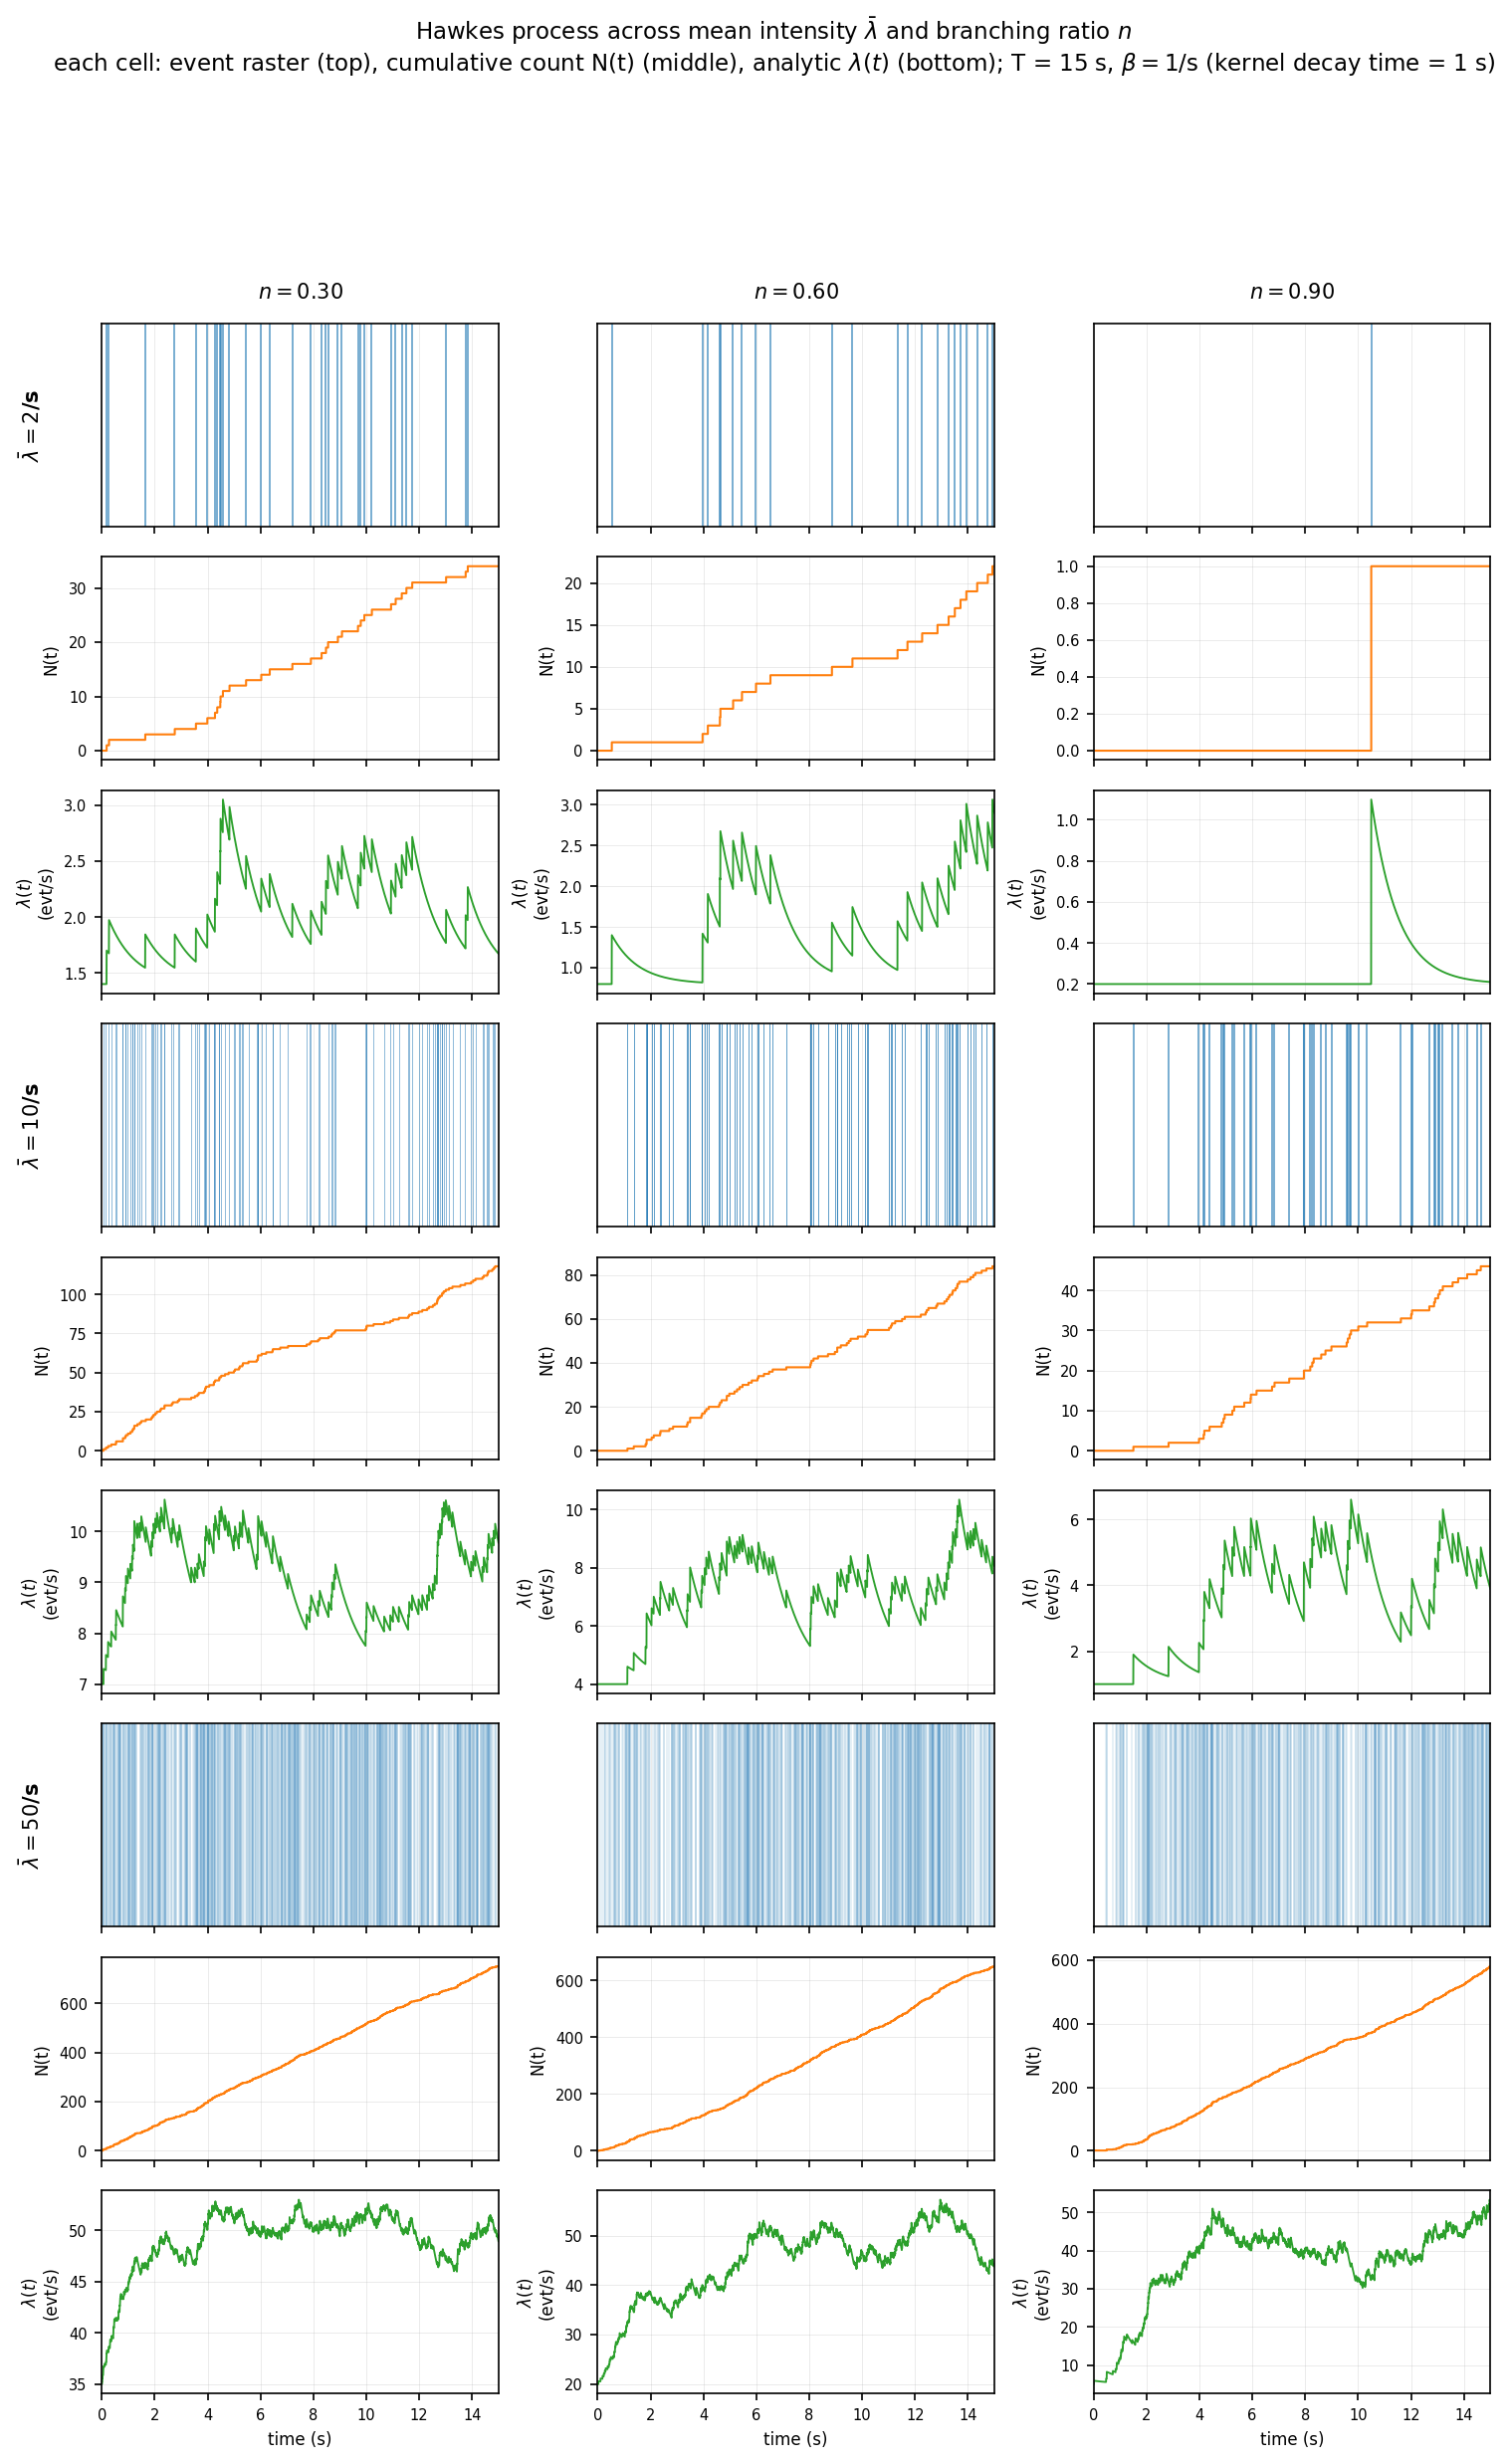
\includegraphics[width=\textwidth]{figs/hawkes_grid_3x3.png}
    \caption{Nine cells, each stacking the event raster (top), cumulative count $N(t)$ (middle), and analytic $\lambda(t)$ (bottom). Rows: mean intensity $\bar\lambda \in \{2, 10, 50\}$ events/s. Columns: branching ratio $n \in \{0.30, 0.60, 0.90\}$. Simulated by Ogata thinning over $15\,\mathrm{s}$ at $\beta = 1/$s. Generator: \texttt{arrival\_paper/make\_hawkes\_grid.py} (RNG seed pinned per cell for reproducibility).}
    \label{fig:hawkes-grid}
\end{figure}

\paragraph{The critical boundary.} At $n = 1$ exactly, the formula $\bar\lambda = \mu / (1 - n)$ diverges. On any finite window the process still fires finitely often, but the variance of $N(T)$ grows superlinearly with $T$. At $n > 1$ the process is supercritical and diverges in finite time; a well-behaved MLE on real data never returns $n > 1$ on a stable session. If a fit lands there it signals estimator instability, non-stationarity, or a mis-specified kernel. Our optimiser constrains $\alpha < \beta$ at the boundary and reports fits that hit the boundary as unreliable. Empirically, Filimonov--Sornette report $n \approx 0.85$--$0.95$ on ES over the 2000s--2010s; our own pilot on NQH5 2025-03-10 lands at $n = 0.90$, consistent with the near-critical-but-stable regime.

\subsection{Why Hawkes captures CME MDP3 and Poisson doesn't}
\label{app:pp-why-hawkes}

Three data signatures that a Poisson (or any renewal) process cannot produce, but Hawkes with $n$ close to 1 produces naturally:

\emph{(i) Very short interarrival gaps.} On ES/NQ book streams roughly 60--85\% of gaps are shorter than one-tenth of the mean gap. For any exponential the corresponding number is $1 - e^{-0.1} \approx 9.52\%$. Hawkes produces the excess of short gaps because each arrival transiently raises $\lambda$.

\emph{(ii) Positive gap autocorrelation.} For a Hawkes process $\mathrm{Corr}(\Delta_i, \Delta_{i+k}) > 0$ at every lag $k$. Long gaps cluster with long gaps (quiet periods), short with short (bursty periods). Renewal has i.i.d.\ gaps by definition, so the corresponding correlation is zero at every lag. Only self-excitation can produce positive lag-$k$ gap correlation.

\emph{(iii) Persistent burstiness across timescales.} The Fano factor $F(T)$ rises with the window size $T$ on a Hawkes process; on Poisson or any renewal it stays constant. Clustering isn't a single-timescale phenomenon --- it looks self-similar over decades of $T$.

\subsection{Fano factor: measuring dispersion of counts}
\label{app:pp-fano}

For a chosen window length $T$, chop the observation interval $[0, \tau_{\mathrm{end}}]$ into $K = \lfloor \tau_{\mathrm{end}}/T \rfloor$ disjoint bins. Let $C_k = N(kT) - N((k-1)T)$ be the count in bin $k$. The Fano factor at window $T$ is
$$F(T) = \frac{\mathrm{Var}[C_k]}{\mathrm{E}[C_k]}.$$
Poisson: $F(T) = 1$ for every $T$. This is the definitive Poisson signature. Hawkes / clustered: $F(T) > 1$, typically growing with $T$. Renewal: $F(T) \to 1$ as $T \to \infty$ because windows contain many i.i.d.\ gaps and the CLT kicks in. Rising Fano at large $T$ is therefore a Hawkes signature, not just a renewal signature. Origin: Fano (1947) in cosmic-ray physics.

\begin{figure}[H]
    \centering
    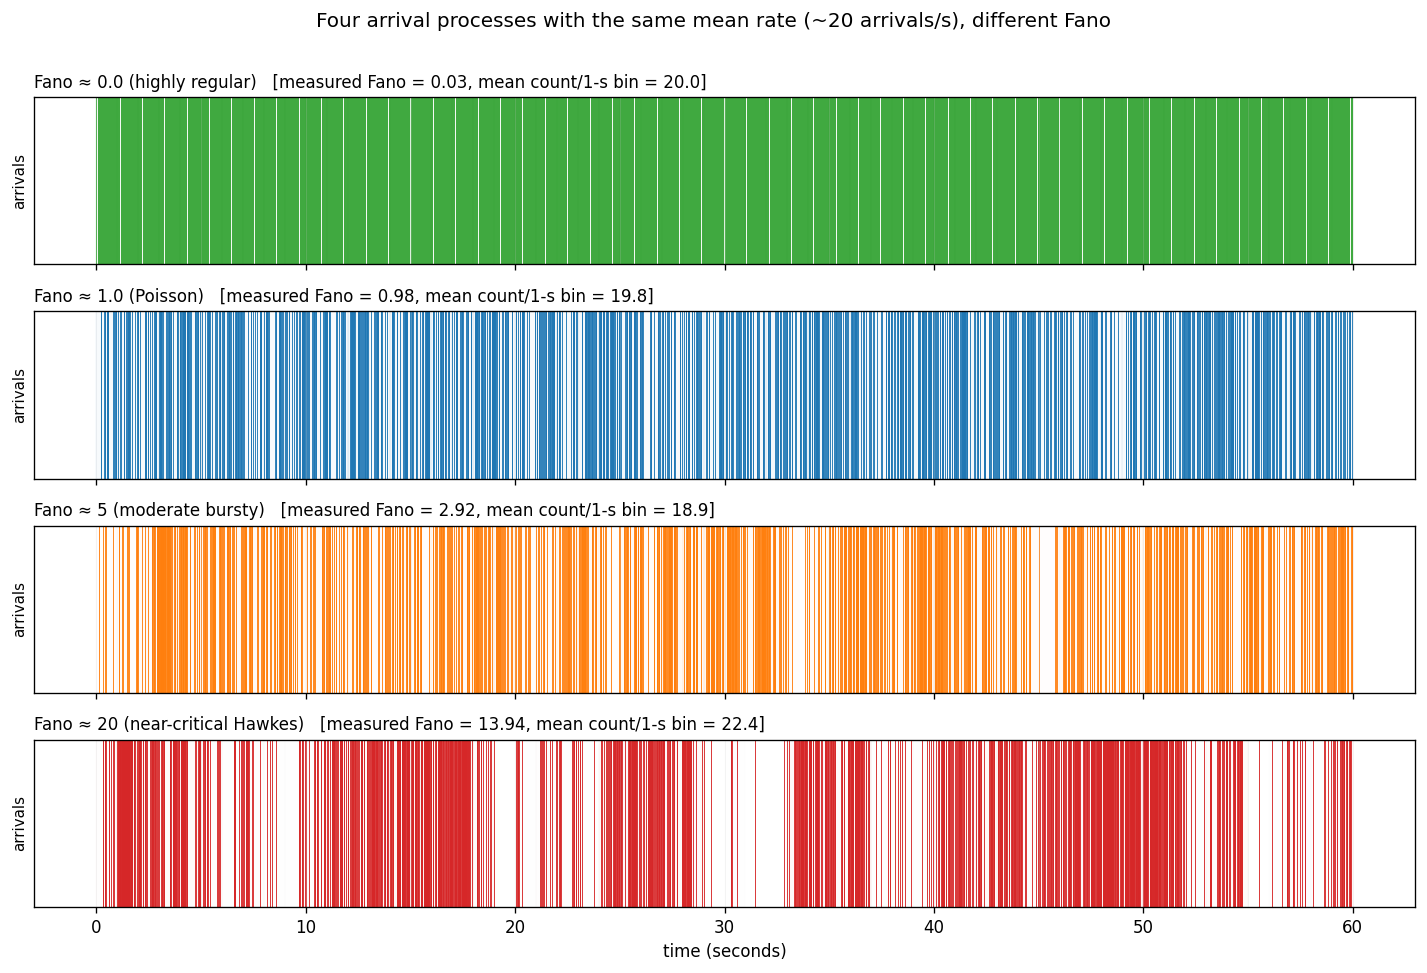
\includegraphics[width=\textwidth]{figs/rasters_by_fano.png}
    \caption{Same mean rate ($\sim 20$/s), four different processes. Top row ($F \approx 0$, highly regular): near-lattice cadence, bin counts nearly equal. Second row ($F \approx 1$, Poisson): the reference --- ``randomly spread'' with mildly uneven bin counts. Third row ($F \approx 3$, moderate Hawkes): visible clumping, bins 5--10 or 30--40. Bottom row ($F \approx 14$, near-critical Hawkes): pronounced bursts and long quiet stretches, bin counts from near zero to 50$+$.}
    \label{fig:rasters-fano}
\end{figure}

\begin{figure}[H]
    \centering
    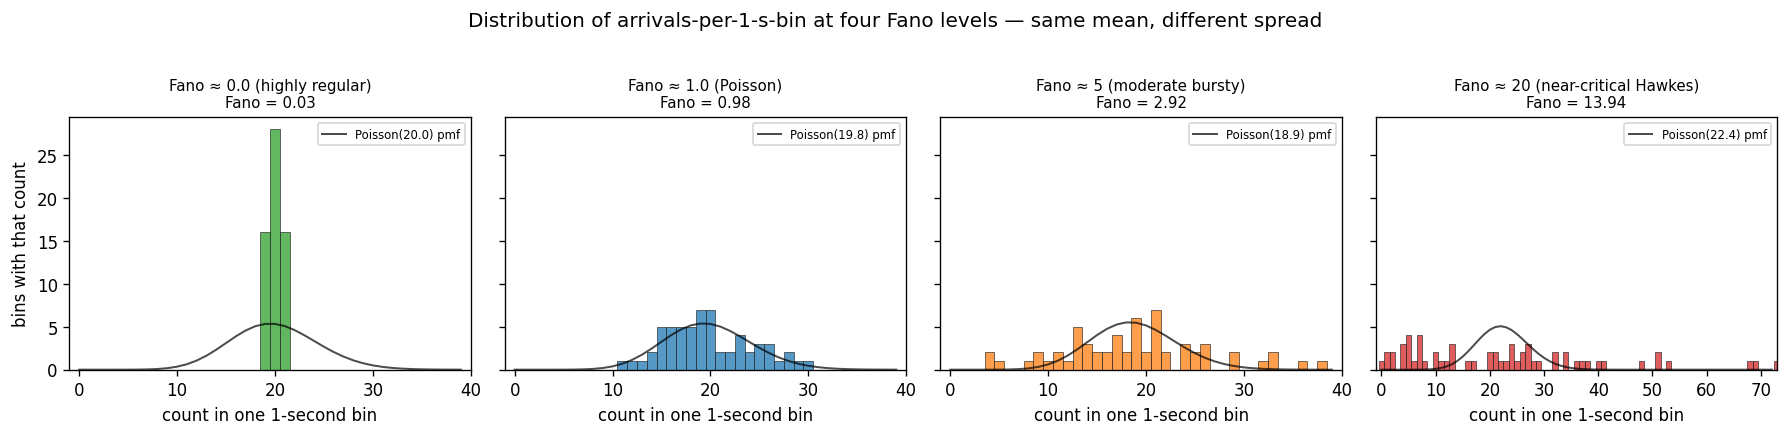
\includegraphics[width=\textwidth]{figs/count_hists_by_fano.png}
    \caption{Empirical distribution of arrivals per 1-second bin (bars) with Poisson pmf at same mean overlaid (curve). $F \approx 0$: histogram much narrower than Poisson --- sub-Poisson. $F \approx 1$: matches Poisson pmf. $F > 1$: wider than Poisson, extra mass in both tails --- what CME MDP3 looks like, shifted much further right ($F(1\,\mathrm{s})$ empirically 10--70 on ES/NQ MBO adds).}
    \label{fig:counthist-fano}
\end{figure}

\subsection{Hurst exponent: how burstiness scales with timescale}
\label{app:pp-hurst}

For a Hawkes-like process near criticality the Fano factor scales as a power law in the window size:
$$F(T) \sim T^{2H - 1},$$
where $H \in [0.5, 1)$ is the Hurst exponent. $H = 0.5$ means no long-range dependence (Poisson, renewal); $H > 0.5$ means long-range dependence, self-similar clustering across timescales; $H \to 1$ means extreme long memory. We estimate $H$ by OLS regression of log Fano on log window:
$$\log F(T) = (2H - 1)\log T + c + \varepsilon.$$
The fitted slope equals $2H - 1$, and $H = (\text{slope} + 1)/2$. For CME book feeds we typically observe $H \in [0.65, 0.75]$.

\begin{figure}[H]
    \centering
    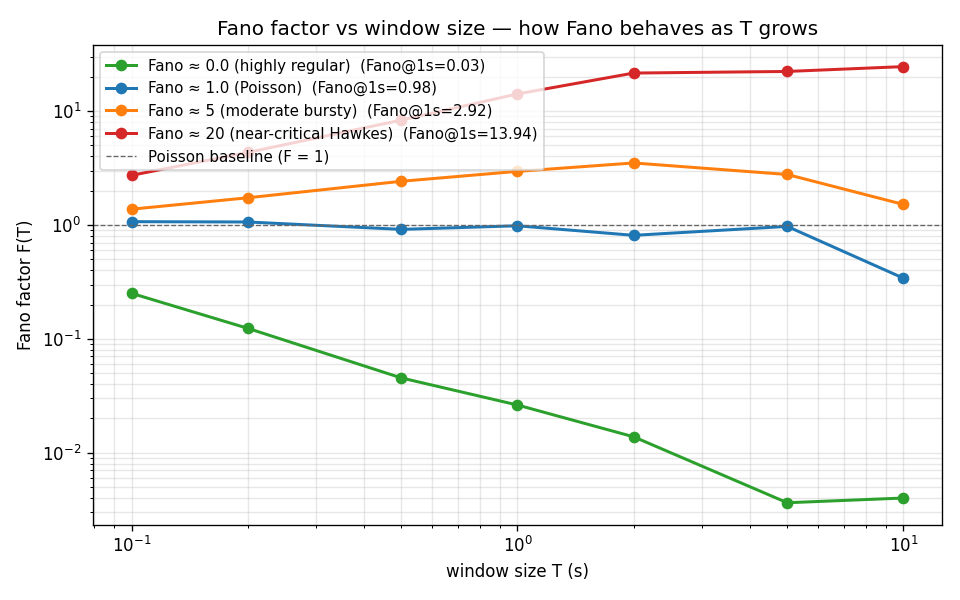
\includegraphics[width=0.75\textwidth]{figs/fano_scaling.png}
    \caption{Log-log $F(T)$ vs $T$ for four simulated processes. Regular: $F(T)$ near zero. Poisson: flat at $F = 1$. Moderate Hawkes: $F(T) > 1$ rising with $T$. Near-critical Hawkes: steep rise --- larger windows see bigger and bigger bursts. Slope of the log-log curve is $2H - 1$; the near-critical curve has slope $\approx 0.5$, corresponding to $H \approx 0.75$.}
    \label{fig:fano-scaling}
\end{figure}

Shuffling the gap sequence (Fisher--Yates permutation) preserves the marginal distribution of gaps exactly but destroys the ordering, thereby destroying any long-range dependence. Under shuffle $H_{\mathrm{shuffled}} \to 0.5$. This is our sharpest test for whether clustering lives in the ordering (Hawkes) or in the marginal (renewal).

\subsection{Notational summary}
\label{app:pp-notation}

\begin{center}
\begin{tabular}{@{}ll@{}}
\toprule
symbol & meaning \\
\midrule
$\Omega$ & sample space of all possible market days \\
$\mathcal{F}$ & $\sigma$-algebra of events \\
$\Pr(A)$ & probability of event $A \in \mathcal{F}$ \\
$\mathcal{F}_t$ & everything observable by time $t$ inclusive \\
$\mathcal{F}_{t^-}$ & everything observable strictly before $t$ \\
$t_1, t_2, \ldots$ & random arrival times \\
$N(t)$ & counting process: $\#\{i : t_i \leq t\}$ \\
$\lambda(t \mid \mathcal{F}_{t^-})$ & conditional intensity at $t$, units 1/time \\
$\mu$ & Hawkes background rate \\
$\phi(u)$ & Hawkes kernel \\
$\alpha$ & exp-kernel jump size \\
$\beta$ & exp-kernel decay rate (half-life $= \ln 2 / \beta$) \\
$\gamma$ & marked-Hawkes size exponent \\
$n = \int \phi$ & branching ratio; for exp kernel $n = \alpha/\beta$ \\
$\Delta_i = t_i - t_{i-1}$ & interarrival gap \\
$C_k$ & arrivals in bin $k$ under some window $T$ \\
$F(T)$ & Fano factor $= \mathrm{Var}[C_k] / \mathrm{E}[C_k]$ \\
$H$ & Hurst exponent, $F(T) \sim T^{2H-1}$ \\
$u_i$ & compensator increment $\int_{t_{i-1}}^{t_i} \lambda\, ds$ (\S\ref{app:pp-gof}) \\
\bottomrule
\end{tabular}
\end{center}

\section{Data --- what we compute from and where it lives}
\label{app:data}

\paragraph{Corpus.} CME MDP3 pre-decoded L3 record files (\texttt{.bin}) for ES (chan 310), NQ (chan 318), and BTC (chan 326, extraction in flight for 2025). Path: \texttt{/vast/home/vmayeski/out/bin/\{chan\}/\{chan\}.\{yyyymmdd\}.databento.bin}. Each record carries three ns-precision timestamps:

\begin{itemize}
    \item \texttt{transactTime} --- CME matching engine event time. The true arrival of the market event, stamped by CME's core matching engine and carried unchanged inside the MDP3 message body.
    \item \texttt{sendingTime} --- CME gateway UDP packet header time. Stamped by CME's outbound gateway when it packages matching-engine events into a UDP packet. The difference $\texttt{sendingTime} - \texttt{transactTime}$ measures CME-internal gateway queueing.
    \item \texttt{recv\_time} (on trades) / \texttt{handlerendtim} (on MBO records) --- the pcap wire-arrival timestamp at Databento's colo capture tap. Not our own capture: Databento captures pcaps in their CME-colo, stamps each UDP frame with the NIC-arrival time, and ships those pcaps to us. When we run \texttt{dbento\_pcap\_to\_bin}, \texttt{handler\_if.hpp} copies the pcap frame timestamp directly into the record's \texttt{handlerendtim} field on MBO messages and into \texttt{recv\_time} on trade messages (verified at \texttt{mdp3/include/mdp3/handler\_if.hpp:577,691,771,832} --- \texttt{l3.handlerendtim = recv\_time} unconditionally in the offline path). The field name \texttt{handlerendtim} is a misnomer inherited from the live-handler code path; in the historical corpus it functions as the pcap wire timestamp. The difference $\texttt{handlerendtim} - \texttt{sendingTime}$ measures CME-multicast transit to Databento's colo tap --- a network-only latency, cleanly separated from CME-internal queueing.
\end{itemize}

\paragraph{Important limitation.} The three-timestamp anatomy uses Databento's colo capture time, not our own. So the $\texttt{handlerendtim} - \texttt{sendingTime}$ distribution characterises the CME $\to$ Databento colo path, which is a stable colo-cross-connect path but is not literally the network we would see if we captured elsewhere. For arrival-process characterisation this does not matter --- the ordering and clustering of arrivals is invariant to any small fixed offset. For any latency-magnitude claim we call this out.

\paragraph{Field-name gotcha.} Older \texttt{handler\_if} code paths (live handlers) do write a genuine ``handler finished processing'' timestamp into \texttt{handlerendtim}. In the historical pcap pipeline we use, that same field is repurposed to carry the pcap wire timestamp.

\paragraph{Restrictions.} One front-month securityID per session (highest MBO Adds count in the day, from \texttt{binstats}). Roll days are dropped (front may straddle two contracts). RTH only, 09:30 $\to$ 16:00 ET. Overnight regime is future work. Message types: MBO records (\texttt{add}, \texttt{modify}, \texttt{cancel}, \texttt{execute}) plus MBO-trade records. Instrument-definition records (FDF/ODF/SDF) and volume/statistic records are excluded --- they are exchange bookkeeping, not order-flow arrivals.

\section{Model classes fit in this paper}
\label{app:models}

Three point-process models per (session, stream), in increasing complexity.

\subsection{Unmarked exponential Hawkes (the workhorse)}
\label{app:model-exp}

$$\lambda(t) = \mu + \sum_{t_i < t} \alpha\, e^{-\beta (t - t_i)}.$$
Three parameters: $\mu \geq 0$ (background), $\alpha \geq 0$ (jump), $\beta > 0$ (decay). Branching ratio $n = \alpha/\beta$. The exponential kernel is Markovian: intensity updates recursively in $O(1)$ per arrival, which is what makes the online estimator practical. Prior art (Hardiman--Bouchaud) warns the true kernel on CME data is closer to a power law; exponential is a working approximation over the timescales we care about ($100\,\mathrm{ms}$ --- $60\,\mathrm{s}$) and is the standard first step.

\subsection{Marked exponential Hawkes with size marks}
\label{app:model-marked}

$$\lambda(t) = \mu + \sum_{t_i < t} \alpha\,(1 + s_i)^\gamma\, e^{-\beta (t - t_i)}.$$
$s_i$ is a size mark: message size class (0--2 depending on quote or trade size deciles) or trade \texttt{lastQty}. $\gamma \geq 0$ measures how much larger events excite subsequent arrivals more than smaller events; LR test against the unmarked model verifies whether size marks meaningfully improve fit. Motivation: large trades and quote deletions plausibly carry more information than small ones.

\subsection{Bivariate Hawkes on \{bid-updates, ask-updates\}}
\label{app:model-bivariate}

Two intensities, one per side. Let $a, b \in \{\text{bid}, \text{ask}\}$:
$$\lambda_a(t) = \mu_a + \sum_{b} \sum_{t_i^{(b)} < t} \alpha_{ab}\, e^{-\beta_{ab}(t - t_i^{(b)})}.$$
$\alpha_{ab}$ is a $2 \times 2$ excitation matrix, diagonal terms $\alpha_{bb}, \alpha_{aa}$ = self-excitation, off-diagonal $\alpha_{ab}, \alpha_{ba}$ = cross-excitation. The $2 \times 2$ branching-ratio matrix has entries $K_{ab} = \alpha_{ab}/\beta_{ab}$; spectral radius of $K$ must be strictly less than 1 for stationarity. Cross-terms measure how much bid-side updates drag ask-side flow and vice versa --- the mechanical prediction that ``the book updates on both sides at once during price discovery.'' Underpins the directional signed-markout prediction in the main paper.

\section{Maximum-likelihood estimation}
\label{app:mle}

\subsection{What fitting a Hawkes actually means}
\label{app:mle-plain}

We have one input --- a sorted list of arrival times $t_1 < t_2 < \cdots < t_n$ for one session and one instrument --- and three knobs $(\mu, \alpha, \beta)$:

\begin{itemize}
    \item $\mu$ --- \textbf{exogenous rate}. Even if nothing has happened recently, events arrive at rate $\mu$ per second. Think ``rate at which news arrives''.
    \item $\alpha$ --- \textbf{jump size}. Every time an event happens, the intensity spikes up by $\alpha$. Units events/second. Think ``how much does one message beget others''.
    \item $\beta$ --- \textbf{decay rate}. Each spike from $\alpha$ fades exponentially with time constant $1/\beta$. Units 1/second. Think ``how fast does excitement fade''.
\end{itemize}

Fitting means: turn the three knobs until the model gives the observed timestamps the highest probability. Formally, maximise the log-likelihood \eqref{eq:hawkes-loglik}. Intuitively, if $\alpha$ is too low the model can't explain visible burst-clustering; if $\alpha$ is too high (approaching $\beta$) the model over-predicts explosive clustering; if $\mu$ is too high or too low the model mis-explains quiet periods. The optimiser tries settings until it finds the triple $(\hat\mu, \hat\alpha, \hat\beta)$ that maximises the log-likelihood.

Once we have the fit, we measure: (i) intensity $\lambda(t)$ --- plug $(\hat\mu, \hat\alpha, \hat\beta)$ into the formula to get $\lambda(t)$ at any $t$, high when arrivals have been clustering, low when the market has been quiet; (ii) branching ratio $n = \alpha/\beta$; (iii) long-run mean intensity $\bar\lambda = \mu/(1 - n)$ --- the stationary expected arrival rate, $\mu$ amplified by $1/(1 - n)$ through self-excitation.

\paragraph{Numerical example (NQH5, 2025-03-10).} On the pilot session:
$$\hat\mu = 0.45\ \text{events/s}, \qquad \hat\alpha = 0.068, \qquad \hat\beta = 0.076,$$
giving branching ratio $\hat n = 0.68/0.076 \approx 0.90$ and long-run mean intensity $\bar\lambda \approx 4.5$ events/s. NQ was strongly self-exciting on that session (near-critical), the exogenous news rate was small (0.45/s), and the observed mean rate of $\sim 5/$s was carried mostly by cascading self-excitation rather than fresh news.

\subsection{Log-likelihood}
\label{app:mle-loglik}

Write $\theta$ for the parameter vector ($(\mu, \alpha, \beta)$ for the unmarked model, $(\mu, \alpha, \beta, \gamma)$ for marked, etc.) and $\log L(\theta)$ for the log-likelihood. For a point process with intensity $\lambda(\cdot; \theta)$ observed on $[0, T]$ with events $t_1, \ldots, t_n$, the log-likelihood is standard \citep{ozaki1979}:
\begin{equation}
\log L(\theta) = \sum_{i=1}^n \log \lambda(t_i; \theta) - \int_0^T \lambda(s; \theta)\, ds.
\label{eq:hawkes-loglik}
\end{equation}
The first term rewards high intensity at the times events actually happened; the second (subtracted) term penalises models that predict too many events overall.

For the exponential Hawkes both terms have closed-form $O(n)$ recursions. Introduce
$$R_i = e^{-\beta(t_i - t_{i-1})}(1 + R_{i-1}), \qquad R_0 \equiv 0,$$
so $\lambda(t_i) = \mu + \alpha R_i$ and
$$\sum_{i=1}^n \log \lambda(t_i) = \sum_{i=1}^n \log(\mu + \alpha R_i).$$
The compensator has the closed form
$$\int_0^T \lambda(s)\, ds = \mu T + \frac{\alpha}{\beta}\sum_{i=1}^n\!\big(1 - e^{-\beta(T - t_i)}\big).$$
Marked and bivariate generalisations are analogous.

\subsection{Optimiser}
\label{app:mle-opt}

Python \texttt{scipy.optimize.minimize} with L-BFGS-B (Limited-memory Broyden--Fletcher--Goldfarb--Shanno with box constraints), a quasi-Newton optimiser that climbs the log-likelihood using local gradient information without the full Hessian and enforces our parameter bounds. Analytic gradient supplied. Bounds: $\mu \geq 0$, $\alpha \geq 0$, $\beta > 0$, and for marked $\gamma \geq 0$. Warm-start from method-of-moments initial estimates. Fit time per RTH session on the 72-core box: seconds for the unmarked model, tens of seconds for marked, minutes for bivariate.

\subsection{Numerical stability}
\label{app:mle-stab}

Sub-second precision timestamps must be shifted to a session-relative origin $t_i \leftarrow t_i - t_0$ before optimisation; otherwise the $\exp(-\beta t_i)$ terms underflow for wall-clock ns timestamps. On very active sessions ($n > 10^7$) we sub-sample uniformly to $n \approx 10^6$ for the fit, then verify on the full sequence. Uniform sub-sampling is not stationary-Hawkes-preserving in the strict sense but produces stable parameter estimates in practice.

\section{Diagnostic statistics --- the per-session panel row}
\label{app:diag}

Everything above sets up the vocabulary and the models. This section says: \emph{for one trading session on one stream, this is exactly what we compute}. Run it $731$ days $\times$ $3$ streams (ES/NQ/BTC) and you get the $\sim 2200$-row panel that every downstream result in the paper reads from.

\paragraph{One session, one stream $\to$ one row of the panel.} Each session on each stream produces roughly 25--30 scalars that fit on a single row. The row is written to disk as JSON at \texttt{/vast/home/vmayeski/out/arrival\_paper/fits/\{stream\}/\{yyyymmdd\}.hawkes.json}; the $\sim 2200$ daily rows are concatenated into \texttt{/vast/home/vmayeski/out/arrival\_paper/panels/hawkes\_panel.parquet}. That panel is the paper's empirical evidence base.

\paragraph{Two kinds of statistics: model-free and model-dependent.} Model-free stats (\S\ref{app:diag-marginal}--\S\ref{app:diag-order}) come first as a sanity check --- any point-process reader can reproduce them without fitting anything. Fit-dependent stats (\S\ref{app:diag-nrec}--\S\ref{app:pp-gof}) tell us whether the Hawkes we fit actually explains the data.

\begin{center}
\begin{tabular}{@{}llll@{}}
\toprule
subsection & what it computes & type & scalars \\
\midrule
\S\ref{app:diag-marginal} Marginal-gap stats & CV, quantile ratios, $\Pr(\text{gap}<\text{mean}/10)$ & model-free & $\sim 10$ \\
\S\ref{app:diag-fano} Fano scaling + Hurst & $F(T)$ at 5 windows, $H$ from slope & model-free & $\sim 6$ \\
\S\ref{app:diag-order} Gap ACF + shuffle test & ACF at 5 lags, shuffled $F(5\,\mathrm{s})$, collapse & model-free & $\sim 7$ \\
\S\ref{app:diag-nrec} Branching-ratio recovery & $n$ MLE, $n$ MoM, gap & fit-dependent & $\sim 3$ \\
\S\ref{app:pp-gof} Goodness-of-fit & KS $p$, Ljung-Box $p_{20}$, QQ plot & fit-dependent & $\sim 2$ \\
\bottomrule
\end{tabular}
\end{center}

Baseline expectations under a homogeneous Poisson at the same mean rate are given in parentheses throughout. Departures from those baselines are the paper's evidence.

\subsection{Marginal-gap statistics}
\label{app:diag-marginal}

\begin{itemize}
    \item \textbf{Coefficient of variation:} $\mathrm{CV} = \sigma(\Delta)/\mathrm{E}[\Delta]$ (Poisson: 1.0).
    \item \textbf{Squared CV:} $\mathrm{CV}^2$ (Poisson: 1.0).
    \item \textbf{Quantile ratios:} p10, p50, p90, p99, p99.9 gaps against $\mathrm{Exp}(\text{same mean})$ quantiles $-m \log(1 - p)$. Ratio crosses 1 exactly once for a burst process.
    \item $\Pr(\text{gap} < \text{mean}/10)$: 9.52\% for any exponential; empirically 40--85\% on CME book streams.
    \item \textbf{Instantaneous rate:} mean rate vs rate implied by median gap. $1/\log 2 \approx 1.44 \times$ for any exponential; empirically 14--120$\times$ on CME.
\end{itemize}

\subsection{Count-based statistics --- Fano scaling and Hurst}
\label{app:diag-fano}

Windowed count in the $k$-th bin: $N_T(k) = N(kT) - N((k-1)T)$. Fano at window $T$: $F(T) = \mathrm{Var}[N_T]/\mathrm{E}[N_T]$ (Poisson: 1 at every $T$). Compute $F(T)$ at $T \in \{0.1, 1, 5, 60, 300\}$ seconds. Fit the log-log regression by OLS to extract the Hurst exponent:
$$\log F(T) \approx (2H - 1)\log T + c.$$
$H = 0.5$ Poisson or renewal, $H \in (0.5, 1)$ long-range dependence characteristic of Hawkes, $H > 1$ non-stationary or diverging variance.

\subsection{Ordering statistics --- gap ACF and shuffle test}
\label{app:diag-order}

Renewal processes with heavy-tailed marginals can produce large CV and moderate Fano without any ordering-driven clustering. To separate the two:

\begin{itemize}
    \item \textbf{Gap ACF} at lags 1, 2, 3, 5, 10. Positive at all lags means long-gap-follows-long-gap.
    \item \textbf{Fisher--Yates shuffle:} seeded permutation of the gap sequence preserves the marginal exactly and destroys the ordering. Recompute $F(5\,\mathrm{s})$ and $H$ on the shuffled sequence. The collapse ratio
    $$\text{collapse} = \frac{F_{\text{original}}(5\,\mathrm{s})}{F_{\text{shuffled}}(5\,\mathrm{s})}$$
    measures how much clustering lives in the ordering versus the marginal. Near 1 = renewal; much greater than 1 (empirically 3--19$\times$ on ES/NQ book streams) = Hawkes. The shuffle is the definitive test: renewal is invariant under shuffle, Hawkes is not.
\end{itemize}

\subsection{Branching-ratio recovery}
\label{app:diag-nrec}

For fitted Hawkes, $n = \alpha/\beta$ directly from the fit. Sanity check against the method-of-moments estimator, which is model-free and uses only the Fano ceiling:
$$n_{\mathrm{MoM}} \leq 1 - \frac{1}{\sqrt{F(T \to \infty)}}.$$
Discrepancy larger than 10\% is a red flag for either misspecification (wrong kernel family) or non-stationarity within the session.

\subsection{Goodness-of-fit --- time-rescaling}
\label{app:pp-gof}

The time-rescaling theorem is a classical result: if we knew the true intensity $\lambda(\cdot)$, integrating it between consecutive events gives compensator increments
$$u_i = \int_{t_{i-1}}^{t_i} \lambda(s)\, ds$$
that are i.i.d.\ $\mathrm{Exp}(1)$ under the correct model. In practice we transform back to uniform via $p_i = 1 - e^{-u_i}$, which should be i.i.d.\ $U(0, 1)$ under the correct model. We then apply:

\begin{itemize}
    \item \textbf{Kolmogorov--Smirnov test} against $U(0, 1)$. Compares the empirical CDF to the target CDF; the statistic is the maximum absolute gap. Small $p$ means the model does not fit. Report $p_{\mathrm{KS}}$ per session.
    \item \textbf{Ljung--Box test} on the $u_i$ for serial correlation --- a joint test that the first several autocorrelations are zero. Small $p$ flags remaining autocorrelation. Report $p_{\mathrm{LB}}$ at lag 20.
    \item \textbf{QQ plot} on $\mathrm{Exp}(1)$ --- plot each residual's rank against its expected $\mathrm{Exp}(1)$ quantile; points fall on $y = x$ if the model fits. Visual, one representative session per stream in the paper.
\end{itemize}

Empirical target: $p_{\mathrm{KS}} > 0.05$ on $\geq 80\%$ of sessions. Failure at this rate on a given stream would indicate the exponential kernel is too restrictive and we would move to a power-law kernel (Hardiman--Bouchaud), a mixture of exponentials, or a marked model.


\section{Exponential-Hawkes maximum-likelihood estimation}
\label{app:hawkes}

The Ogata log-likelihood recursion and the closed-form compensator, with the numerical stopping criterion used, are documented in the companion code.

\section{Reference implementation of the Lindley recursion}
\label{app:lindley}

The Lindley recursion \eqref{eq:lindley-d}--\eqref{eq:lindley-w} as implemented in the measurement pipeline, with unit tests establishing the identity of Section~\ref{sec:queue-identity}.

\section{Full grid heatmaps}
\label{app:grid}

Full $5 \times 5$ grid heatmaps for the three latency tails crossed with \{absolute, ratio\}, and the cell-mass heatmap.

\section{Reference implementation of the simulator upgrade}
\label{app:refimpl}

The two-queue upgrade of Section~\ref{sec:upgrade} is implemented in the \kasparhft{} order-book actor. The two release rules coexist under a compile-time guard: with the guard off, the release rule is the historical constant-delay rule and the simulator's output is bit-identical to the version cited in \citep{mayeski2026shadowpov}; with the guard on, the release rule is the Lindley recursion of equations~\eqref{eq:lindley-d}--\eqref{eq:lindley-w} on the two independent queues (inbound and outbound). The two scalar service times $s_{\mathrm{in}}$ and $s_{\mathrm{out}}$ are read from a configuration file at process start. A regression-test suite exercises: (i) bit-identical output against the previous release with the guard off; (ii) round-trip identity on a synthetic saturated arrival stream against a Python reference; and (iii) determinism across a fixed random seed at high $\bar\lambda$ and $n$.

\section{Companion code repository}
\label{app:code}

\subsection*{Repositories}

The full source used to produce this paper's tables and figures ships in two repositories:

\begin{itemize}
    \item \texttt{kaspar-hft} --- the C++20 actor-based MDP3 replay simulator \citep{mayeski_actorhft}. Includes the SBE decoders, the order-book actor, the tape-recorder actors, the two-queue G/D/1 upgrade of Section~\ref{sec:upgrade}, and the driver binaries \texttt{msgtape} and \texttt{bin\_replay\_bbo}. Build system: GNU make with per-library sub-makes; requires a C++20 toolchain (g++ 11+ or clang 14+) and the CME SBE templates, which are generated by the build.
    \item \texttt{kaspar\_arrival} --- the Python 3.10+ analysis package. Modules:
    \begin{itemize}
        \item \texttt{hawkes\_smoke} --- exponential-Hawkes MLE via the Ogata recursion, closed-form compensator integral, and L-BFGS-B optimisation using \texttt{scipy.optimize.minimize}.
        \item \texttt{hourly\_panel} --- per-window panel builder consuming a session's message tape and emitting one row per surviving window (Section~\ref{sec:pipeline-panel}).
        \item \texttt{grid\_scan} --- corpus-level aggregator producing the equal-quantile grid on $(\bar\lambda, n)$ and the heatmap PDFs.
        \item \texttt{qlen\_sweep\_by\_intensity} --- G/D/1 sweep over the service-time parameter $s$ conditional on each grid cell (Section~\ref{sec:queue-sweep}).
        \item \texttt{front\_contract} --- daily front-month selection from open interest and volume, with roll-window exclusion.
        \item \texttt{fill\_tape} and \texttt{packet\_tape} --- one-pass Python builders producing the two Python-derived tapes described in Section~\ref{sec:pipeline-kaspar}.
    \end{itemize}
    Runtime dependencies: NumPy, SciPy, Pandas, PyArrow. All optional.
\end{itemize}

Both repositories are released under the MIT licence. The final URLs and release tag corresponding to the version of this paper are inserted at typesetting time.

\subsection*{Batch driver}

The parallel batch script \texttt{run\_panel\_batch.sh} runs the panel builder across the corpus. It reads a list of session dates, invokes one \texttt{hourly\_panel} instance per session across 72 cores using GNU parallel, and consolidates the per-session Parquet files into a single corpus panel. A companion script \texttt{run\_tape\_batch.sh} does the same for the C++ recorder binaries on the raw \texttt{.bin} archive.

\subsection*{Pinned versions}

The exact commit of each repository used to produce a given release of this paper is recorded in a version manifest file (\texttt{VERSION.txt}) shipped with the release. A reader who checks out the two repositories at those commits, installs the pinned Python dependencies from the accompanying \texttt{requirements.txt}, and follows the seven-step runbook of Section~\ref{sec:pipeline-repro} will reproduce every numerical value reported here.

\nocite{bacrydelattre2013,filimonovsornette2012,rambaldibacrymuzy2018}

\begin{thebibliography}{99}

\bibitem[Hawkes(1971)]{hawkes1971spectra}
Hawkes, A. G. (1971).
\newblock Spectra of some self-exciting and mutually exciting point processes.
\newblock \emph{Biometrika} 58(1), 83--90.

\bibitem[Mayeski(preparation)]{mayeski_actorhft}
Mayeski, V. (in preparation).
\newblock An actor-model execution framework for high-frequency trading.
\newblock M2 Tech Technical Note, in preparation.
\newblock \emph{Placeholder --- full citation to be supplied.}

\bibitem[Konishi and Makimoto(2001)]{konishimakimoto2001pov}
Konishi, H., Makimoto, N. (2001).
\newblock Optimal slice of a block trade.
\newblock \emph{Journal of Risk} 3(4), 33--51.

\bibitem[Mayeski(2026)]{mayeski2026shadowpov}
Mayeski, V. (2026).
\newblock \shadowpov{}: a percentage-of-volume execution algorithm for CME futures.
\newblock M2 Tech Technical Note, in preparation.
\newblock \emph{Placeholder --- full citation to be supplied.}

\bibitem[Byrd et~al.(2020)]{byrd2020abides}
Byrd, D., Hybinette, M., Balch, T. (2020).
ABIDES: Towards high-fidelity multi-agent market simulation.
ACM SIGSIM-PADS; arXiv 1904.12066.

\bibitem[Amrouni et~al.(2021)]{amrouni2021abidesgym}
Amrouni, S., Moulin, A., Vann, J., Vyetrenko, S., Balch, T., Veloso, M. (2021).
ABIDES-Gym: Gym environments for multi-agent discrete-event simulation and application to financial markets.
ICAIF; arXiv 2110.14771.

\bibitem[Mascioli and Wellman(2024)]{masciolwellman2024pymarketsim}
Mascioli, C., Wellman, M. P. (2024).
PyMarketSim: A strategic agent-based simulator for limit-order-book markets.
ICAIF.

\bibitem[Belcak et~al.(2020)]{belcak2020maxe}
Belcak, P., Calliess, J.-P., Zohren, S. (2020).
Fast agent-based simulation framework of limit order books with applications to pro-rata markets and the study of latency effects (MAXE).
Oxford-Man Institute of Quantitative Finance.

\bibitem[Cliff(2018)]{cliff2018bse}
Cliff, D. (2018).
BSE: A minimal simulation of a limit-order-book stock exchange.
arXiv 1809.06027.

\bibitem[Miles and Cliff(2019)]{milescliff2019dbse}
Miles, S., Cliff, D. (2019).
A cloud-native globally distributed financial exchange simulator (DBSE).
European Modelling and Simulation Symposium; arXiv 1909.12926.

\bibitem[Jericevich et~al.(2022)]{jericevich2022cointossx}
Jericevich, I., Chang, P., Gebbie, T. (2022).
CoinTossX: An open-source low-latency high-throughput matching engine.
SoftwareX 17; arXiv 2102.10925.

\bibitem[Huang and Polak(2011)]{huangpolak2011lobster}
Huang, R., Polak, T. (2011).
LOBSTER: Limit-order-book system for the efficient reconstruction of NASDAQ ITCH data.

\bibitem[Frey et~al.(2023)]{frey2023jaxlob}
Frey, S., Li, K., Nagy, P., Sapora, S., Lu, C., Zohren, S., Foerster, J., Zheng, S. (2023).
JAX-LOB: A GPU-accelerated limit-order-book simulator for reinforcement learning.
ICAIF; arXiv 2308.13289.

\bibitem[Mohl et~al.(2025)]{mohl2025jaxmarl}
Mohl, V., et al. (2025).
JaxMARL-HFT: Multi-agent reinforcement learning for high-frequency trading on tape replay.
arXiv 2511.02136.

\bibitem[Jerome et~al.(2023)]{jerome2023mbtgym}
Jerome, J., Sabate-Vidales, M., \v{S}i\v{s}ka, D., Szpruch, \L. (2023).
mbt\_gym: A modular training gym for market-making and execution reinforcement learning.
arXiv 2209.07823.

\bibitem[Noble et~al.(2026)]{noble2026reality}
Noble, K., Rosenbaum, M., Souilmi, W. (2026).
\newblock Bridging the Reality Gap in LOB Simulation.
\newblock arXiv 2603.24137.

Bridging the reality gap in limit-order-book simulation.
arXiv 2603.24137.

\bibitem[El Karmi(2025)]{elkarmi2025hawkeslob}
El Karmi, S. (2025).
A deterministic limit-order-book simulator with Hawkes-driven order flow.
arXiv 2510.08085.

\bibitem[Berti et~al.(2025)]{berti2025deepmarket}
Berti, L., et al. (2025).
DeepMarket / TRADES: a diffusion generator for realistic order-flow simulation on ABIDES.
arXiv 2502.07071.

\bibitem[StockSharp community(2013)]{stocksharp}
StockSharp community (2013--).
StockSharp trading and algorithmic trading platform.
\url{https://github.com/StockSharp/StockSharp}.

\bibitem[Daw and Pender(2018a)]{dawpender2018queues}
Daw, A., Pender, J. (2018).
Queues driven by Hawkes processes.
Stochastic Systems 8(3), 192--229.

\bibitem[Baccelli et~al.(2005)]{baccellifosslelarge2005}
Baccelli, F., Foss, S., Lelarge, M. (2005).
Tail asymptotics for monotone-separable networks.
Journal of Applied Probability 42(3), 793--812; arXiv:math/0510117.

\bibitem[Foss and Korshunov(2000)]{fosskorshunov2000}
Foss, S., Korshunov, D. (2000).
Steady-state asymptotics for tandem, split-match and other feedforward queues with heavy-tailed service.
Queueing Systems 35, 65--80.

\bibitem[Gao and Zhu(2024)]{gaozhu2024statedep}
Gao, X., Zhu, L. (2024).
Single-server queues with state-dependent Hawkes arrivals.
Mathematics of Operations Research; arXiv 2311.02577.

\bibitem[Koops et~al.(2018)]{koopsboxmamandjes2018}
Koops, D. T., Boxma, O. J., Mandjes, M. R. H. (2018).
Infinite-server queues with Hawkes arrivals.
Queueing Systems 92, 27--52.

\bibitem[Chen and Blanchet(2021)]{chenblanchet2021}
Chen, X., Blanchet, J. (2021).
Perfect sampling of Hawkes processes and queues with Hawkes arrivals.
Stochastic Systems 11(3), 264--283; arXiv 2002.06369.

\bibitem[Heindl(2001)]{heindl2001mmpp}
Heindl, A. (2001).
Decomposition of general tandem queueing networks with MMPP input.
Performance Evaluation 44(1--4), 5--23.

\bibitem[Kim and Chydzinski(2002)]{kimchydzinski2002mmpp}
Kim, Y. H., Chydzinski, A. (2002).
Connection-wise end-to-end performance analysis of queueing networks with MMPP inputs.
Performance Evaluation 47(2--3), 137--156.

\bibitem[Gao et~al.(2024)]{gao2024hawkessplit}
Gao, X., Zhu, L., et~al. (2024).
Heavy-traffic limits for parallel single-server queues with randomly split Hawkes arrivals.
Working paper.

\bibitem[Dean and Barroso(2013)]{deanbarroso2013tailatscale}
Dean, J., Barroso, L. A. (2013).
The tail at scale.
Communications of the ACM 56(2), 74--80.

\bibitem[Ozaki(1979)]{ozaki1979}
Ozaki, T. (1979).
Maximum likelihood estimation of Hawkes' self-exciting point processes.
Annals of the Institute of Statistical Mathematics 31(1), 145--155.

\bibitem[Zhao et~al.(2023)]{zhao2023parsimon}
Zhao, K., Alizadeh, M., Pan, R., Ports, D. R. K., Perry, J., Yang, X., et~al. (2023).
Parsimon: Scalable tail latency estimation for data center networks.
NSDI 2023.

\bibitem[Coletta et~al.(2022)]{coletta2022cgan}
Coletta, A., Prata, M., Conti, M., Mercuri, E., Nucciarelli, A., Somacal, M., Vyetrenko, S., Balch, T. (2022).
Towards realistic market simulation: A generative-adversarial world agent for ABIDES.
ICAIF.

\bibitem[Vyetrenko et~al.(2020)]{vyetrenko2020getreal}
Vyetrenko, S., Byrd, D., Petosa, N., Mahfouz, M., Dervovic, D., Veloso, M., Balch, T. (2020).
Get real: realism metrics for robust LOB market simulations.
ICAIF.

\bibitem[Wah and Wellman(2016)]{wahwellman2016}
Wah, E., Wellman, M. P. (2016).
Latency arbitrage in fragmented markets: A strategic agent-based analysis.
Algorithmic Finance 5(3--4), 69--93.

\bibitem[Aquilina et~al.(2022)]{aquilina2022arms}
Aquilina, M., Budish, E., O'Neill, P. (2022).
Quantifying the high-frequency trading ``arms race''.
Quarterly Journal of Economics 137(1), 493--564.

\bibitem[Stoikov et~al.(2020)]{stoikov2020imbalance}
Stoikov, S., et al. (2020).
The importance of low latency to order-book-imbalance strategies.
arXiv 2006.08682.

\bibitem[Daw and Pender(2018b)]{dawpender2018queuehawkes}
Daw, A., Pender, J. (2018).
The queue-Hawkes process: ephemeral self-excitement.
Winter Simulation Conference; arXiv 1811.04282.

\bibitem[Bacry et~al.(2015a)]{bacry2015review}
Bacry, E., Mastromatteo, I., Muzy, J.-F. (2015).
Hawkes processes in finance.
Market Microstructure and Liquidity 1(1).

\bibitem[Cartea et~al.(2014)]{carteajaimungalricci2014}
Cartea, \'A., Jaimungal, S., Ricci, J. (2014).
Buying low, selling high: A high-frequency trading perspective.
SIAM Journal on Financial Mathematics 5(1), 415--444.

\bibitem[Rambaldi et~al.(2017)]{rambaldi2017volume}
Rambaldi, M., Bacry, E., Lillo, F. (2017).
The role of volume in order-book dynamics: A multivariate Hawkes-process analysis.
arXiv 1602.07663.

\bibitem[Bacry et~al.(2015b)]{bacrygaiffasmuzy2015}
Bacry, E., Ga\"iffas, S., Muzy, J.-F. (2015).
State-dependent Hawkes processes for limit-order-book modelling.

\bibitem[Moallemi and Sa\u{g}lam(2013)]{moallemisaglam2013}
Moallemi, C. C., Sa\u{g}lam, M. (2013).
The cost of latency in high-frequency trading.
Operations Research 61(5), 1070--1086.

\bibitem[Bergault et~al.(2020)]{bergault2020}
Bergault, P., Drissi, F., Gu\'eant, O. (2020).
Multi-asset optimal execution and statistical arbitrage strategies under Ornstein-Uhlenbeck dynamics.
arXiv 1806.05849.

\bibitem[Bonart and Gould(2017)]{bonartgould2017}
Bonart, J., Gould, M. D. (2017).
Latency and liquidity provision in a limit order book.
Quantitative Finance 17(10), 1601--1616.

\bibitem[Cartea et~al.(2021)]{carteajaimungalsb2021}
Cartea, \'A., Jaimungal, S., S\'anchez-Betancourt, L. (2021).
Latency and liquidity risk.
International Journal of Theoretical and Applied Finance; arXiv 1908.03281.

\bibitem[Cartea and S\'anchez-Betancourt(2021)]{carteasb2021shadow}
Cartea, \'A., S\'anchez-Betancourt, L. (2021).
The shadow price of latency: Improving intraday fill ratios in FX.
SIAM Journal on Financial Mathematics.

\bibitem[Cartea and S\'anchez-Betancourt(2022)]{carteasb2022stochastic}
Cartea, \'A., S\'anchez-Betancourt, L. (2022).
Optimal execution with stochastic delay.
Finance and Stochastics.

\bibitem[Sun et~al.(2024)]{sun2024}
Sun, R., et al. (2024).
Market simulation under adverse selection.
arXiv 2409.12721.

\bibitem[Hardiman et~al.(2013)]{hardiman2013}
Hardiman, S. J., Bercot, N., Bouchaud, J.-P. (2013).
Critical reflexivity in financial markets.
European Physical Journal B 86(10), 442.

\bibitem[Bacry et~al.(2013)]{bacrydelattre2013}
Bacry, E., Delattre, S., Hoffmann, M., Muzy, J.-F. (2013).
Modelling microstructure noise with mutually exciting point processes.
Quantitative Finance 13(1), 65--77.

\bibitem[Filimonov and Sornette(2012)]{filimonovsornette2012}
Filimonov, V., Sornette, D. (2012).
Quantifying reflexivity in financial markets.
Physical Review E 85(5).

\bibitem[Rambaldi et~al.(2018)]{rambaldibacrymuzy2018}
Rambaldi, M., Bacry, E., Muzy, J.-F. (2018).
Modelling realized covariance and returns via a matrix-variate Hawkes process.
SIAM Journal on Financial Mathematics.

\end{thebibliography}

\end{document}
